\documentclass[final]{ucbthesis}
\usepackage[table]{xcolor}
\usepackage{graphicx}
\usepackage{subcaption}
\usepackage[obeyFinal]{todonotes}
\graphicspath{{img/}}

\usepackage{silence}
\WarningFilter{ctable}{Transparency}
\usepackage{samstyle}

\bibliography{bib}

\begin{document}

\title{
    Measurement of the Neutrino Mixing Angle $\thetaot{}$
    Using Neutron Capture on Hydrogen
    at the Daya Bay Reactor Neutrino Experiment
}
\author{Samuel Joseph Kohn}
\degreesemester{Spring}
\degreeyear{2021}
\degree{Doctor of Philosophy}
\chair{Professor Kam-Biu Luk}
\othermembers{
    Professor Trevor Darrell \\
    Professor Yury Kolomensky
}
\numberofmembers{3}
\field{Physics}

\maketitle
\copyrightpage

\begin{abstract}
    A measurement of the smallest neutrino mixing angle, \thetaot{},
    by observations of reactor \nuebar{} disappearance
    at the Daya Bay Reactor Neutrino Experiment over 1958 days, is described.
    Eight identically-designed antineutrino detectors (ADs) monitored the \nuebar{} flux
    produced by six \SI{2.9}{\GW\of{th}} nuclear reactors,
    with four ADs located close to the reactors
    ($\sim$\SIrange[range-phrase = --]{350}{600}{\m})
    monitoring the unoscillated flux,
    and four ADs located far from the reactors
    ($\sim$\SIrange[range-phrase = --]{1500}{1950}{\m})
    observing the oscillated flux.
    Inverse beta decay events were identified based on the coincidence
    of the prompt positron annihilation and the delayed neutron capture on hydrogen
    within the organic liquid scintillator target of each AD.
    A selection based on both the time delay and distance
    between the prompt and delayed events
    allowed for a strong suppression of the largest background,
    uncorrelated (accidental) coincidences of decays of radiocontaminants in the ADs.
    Differences in detection efficiency between ADs
    were constrained to within \SI{0.66}{\percent},
    dominated by the AD-uncorrelated uncertainty
    of the coincidence distance and time criteria.
    Comparison of the near AD and far AD observations,
    with appropriate adjustments for
    detector livetimes, AD-reactor baselines, and backgrounds,
    revealed a disappearance signal
    with minimal dependence on reactor modeling and detector response.
    A $\chi^2$ expression
    with nuisance parameters was constructed to model the impact of \thetaot{}
    and systematic uncertainties on the predicted far AD observations
    given the near AD observations as input.
    A fit was performed using the exact three-flavor probability
    for \nuebar{} disappearance
    assuming the normal mass ordering,
    and found $\sin^22\thetaot = 0.0731^{+0.0087}_{-0.0089}$.
\end{abstract}


\begin{frontmatter}
    \begin{dedication}
\null\vfil
\begin{center}
    \emph{
    To my parents, Ruth and Arthur,\\
    and my wife, Jaime
}
\end{center}
\vfil\null
\end{dedication}

    \tableofcontents
    \clearpage
    \listoffigures
    \clearpage
    \listoftables
    \clearpage
    \begin{acknowledgements}


    This dissertation would not have been possible
    without the support of many mentors, colleagues, friends and family.
    To my advisor, Professor Kam-Biu Luk,
    thank you for guiding me through my growth as a researcher these past seven years.
    Your curiosity is contagious:
    even before I officially joined your research group,
    you pitched me on all sorts of side projects
    like the laser electron accelerator
    and water-based liquid scintillator.
    I appreciate that you supported my detour into the LArPix project,
    where I was able to develop valuable hardware and electronics experience.
    When I faced setbacks, you reminded me that
    a main goal of being a researcher is to have fun.

    To my colleagues in the LBNL Neutrino Group over the years,
    Herb, Dan, Cheng-Ju, Brooke, Chris, Yasu, Patrick, Matt, Henoch and Peter:
    I could not have asked for better research collaborators / lunch companions.
    Breaking bread with you every day was one of the first things I started missing
    at the start of the pandemic.
    Herb, thank you for raising all the questions I could not answer
    and pointing out all the problems with my data that I tried to paper over;
    your zeal for clear answers has made me a better scientist.
    Dan, thank you for your mentorship and leadership on the LArPix project,
    and for helping me to nail down my plans for this dissertation
    at both the beginning and the end of the journey.

    I must thank my undergraduate research advisors,
    Professors Szabolcs Marka and Brian Cole.
    You taught me the foundations for being a successful particle physicist:
    clear and detailed talks, and lots of plots.
    And to my high-school physics teacher, Mr.~Vaughan,
    thank you for making physics seem hard yet doable,
    mysterious yet intuitive.
    Some of your lessons --- particularly ``Step 1: draw a free-body diagram''---
    inform how I approach difficult problems to this day.
    I apologize for including semicolons in this dissertation.

    I would long ago have given up hope of completing this dissertation
    were it not for the support and camaraderie of my friends in Berkeley.
    Neil, Chelsea, Alex, Steve, Kyle, Amy, Matt, Claire, both Chrises, Crystal,
    and Justin:
    from Tuolomne Meadows and Death Valley to Golden Gate Fields and Jupiter,
    we all proved that it really is possible to be a grad student
    and a balanced human being at the same time.
    Thank you all for being there for me, both for the pep talks
    and the celebrations.
    To Simca, thank you for your trust in me as we built
    Respect is Part of Research together to make our department
    a safer place to work.

    My union, UAW Local 2865, gave me opportunities to learn and to lead.
    Thank you to Vetri for bringing me to my first union meeting, and
    to David for having the audacity to invite me to a 2-day organizing training
    just 15 minutes after we first met.
    Garrett, Kavitha, Zach, Greg and Gwen, you all were the reason
    I looked forward to the day-to-day experience of union organizing.

    Mom and Dad, you have supported me literally from Day One.
    You fostered in me a love of learning, a love of music,
    and a love of community.
    Most importantly, you held it together for eight years
    while I worked towards my degree 3000 miles away.
    Thank you for asking whether I'm moving back only once every few phone calls.
    Tom, thank you for shouldering the burden of being the only Kohn brother
    at family gatherings when I wasn't able to fly home.

    To my wife, Jaime, thank you for believing in me,
    for letting me air my frustrations when my code wasn't working,
    for helping me plan my writing schedule,
    for doing \SI{90}{\percent} of the housework while I was
    locked in the office writing,
    for bringing me thesis fuel snacks,
    for planning excursions on my days off,
    for planning meals on my writing days,
    for putting things in perspective when plans went awry,
    for advocating for me to myself when I was too stressed to think straight,
    for learning about my research,
    and for agreeing that we should spend the rest of our lives together.




\end{acknowledgements}

\end{frontmatter}
\chapter{Neutrino Oscillation}
\label{ch:intro}

The study of neutrinos and their oscillations has been the source
of countless surprises in the development of the
Standard Model of particle physics and beyond.
Neutrinos are currently the only particles exhibiting properties
not explained by the Standard Model
which can be studied---not just searched for---on Earth in a laboratory setting.
This chapter will introduce the history of neutrinos
up to the discovery of neutrino oscillation (\cref{sec:history});
describe the modern theoretical understanding of neutrino oscillation
(\cref{sec:osc_intro});
and present the experimental techniques used to study neutrino oscillation,
focusing on those used by the Daya Bay Reactor Neutrino experiment (\cref{sec:experiment_intro}).

\section{History of neutrinos}
\label{sec:history}

The first evidence of neutrinos emerged in the form of
the continuous spectrum of $\beta$ particles
emitted during nuclear decay.
The continuous spectrum was first reported by Chadwick in 1914 \cite{chadwick_beta}.
Additional measurements confirming Chadwick's result accumulated over the next decade.
At the time, $\beta$ decay was thought to be a 2-body decay
of a nucleus $N$ with charge $Z$ and atomic mass $A$:
\begin{equation}\label{eq:old_beta}
    N(A, Z) \to N(A, Z+1) + \beta^-
\end{equation}
Conservation of energy should have uniquely determined the energy
of the outgoing $\beta$ particles for a given decay,
thus producing a monoenergetic spectrum,
as had been observed for $\alpha$ and $\gamma$ decays.
The observed continuous spectrum conflicted with this prediction.
In 1931, rather than sacrifice the principle of conservation of energy,
Pauli proposed the introduction of a light neutral particle
produced during $\beta$ decay that escaped detection
due to a low interaction cross section \cite{pauli_letter}.
The particle, eventually named the neutrino ($\nu$) by Fermi,
provided the additional degree of freedom needed
to maintain conservation of energy and allow for a continuous $\beta$ spectrum
via the 3-body decay
\begin{equation}\label{eq:beta_mid}
    N(A, Z) \to N(A, Z+1) + \beta^- + \nu.
\end{equation}
Subsequent experiments, detailed below,
would reveal the existence of an antineutrino $\bar{\nu}$,
followed by a distinction between neutrino flavors $\nu_e, \nu_\mu,$
and, much later, $\nu_\tau$.
Lepton flavor conservation requires that
the original neutrino proposed to solve
the problem of the continuous $\beta$ spectrum
is actually the electron antineutrino (\nuebar).
Additionally, the discoveries of the proton and neutron
led to the conclusion that $\beta$ decay was the result of
the decay of a single neutron rather than of the nucleus as a whole.
Much later, the discovery of quarks and electroweak vector bosons
further refined the $\beta$ decay process.
The modern understanding of $\beta$ decay is therefore
\begin{align}\label{eq:beta_modern}
    \begin{split}
        n &\to p + e^- + \nuebar \text{ (nucleon level)} \\
        udd &\to uud + W^- \to uud + e^- + \nuebar \text{ (parton level)}.
    \end{split}
\end{align}
This process and its equivalents for $\mu$ and $\tau$
provide the vast majority of opportunities for
experimental investigation of the neutrino to this day.

\subsection{Discovery of the neutrino}
\label{subsec:discovery}

Reines and Cowan were the first to observe the neutrino experimentally in 1956
\cite{reines_cowan}.
They used a liquid scintillator detector to monitor a target of
water with dissolved $\text{CdCl}_2$
placed near the Savannah River Plant nuclear reactor.
The neutrinos were expected to undergo the inverse beta decay (IBD) reaction,
\begin{equation}\label{eq:ibd}
    \nuebar + p \to n + e^+,
\end{equation}
with the proton supplied by a hydrogen nucleus (\isotope[1]{H}) in the water.
The positron would annihilate in the water almost immediately,
producing two $\gamma$ rays which were detected in the liquid scintillator
as a prompt signal.
The neutron would scatter within the target for \SI{\sim5}{\us}
and eventually capture on a Cd nucleus,
triggering the emission of several $\gamma$ rays totaling \SI{9}{\MeV}
due to nuclear de-excitation,
detected as a delayed event by the liquid scintillator.
IBD events were identified by the coincidence of a prompt and delayed event
at a rate of \num{2.88\pm0.22} per hour,
only present when the reactor was powered on.
This experiment was the earliest progenitor of the Daya Bay experiment,
which also observed reactor \nuebar{} using a liquid scintillator detector
and the principle of the prompt-delayed coincidence for IBD events.

\subsection{Difference between \texorpdfstring{$\nu$ and $\bar{\nu}$}{nu and nu-bar}}
\label{subsec:nu_vs_nubar}

Even prior to Reines and Cowan's observation of the neutrino,
Davis was able to provide convincing evidence that
the antineutrino was different from the neutrino \cite{davis_diff_nuebar}.
In 1954, Davis attempted to observe the reaction
\begin{equation}\label{eq:davis_nubar}
    \isotope[37]{Cl} + \bar{\nu} \to \isotope[37]{Ar} + \beta^-.
\end{equation}
If $\nu=\bar{\nu}$, then lepton number conservation could be violated
and the reaction could occur.
A tank containing \SI{3900}{\liter} of $\text{CCl}_4$
was placed in close proximity to the Brookhaven nuclear reactor.
Any \isotope[37]{Ar} produced was extracted using helium gas,
and the resulting gas was monitored using a Geiger counter
to observe the decay of \isotope[37]{Ar} (half-life 35 days).
No decays of \isotope[37]{Ar} were observed over the expected background.
Thus it was concluded that $\nu\neq\bar{\nu}$.

Davis noted in the conclusion of his report that the same experimental setup
could be used to detect neutrinos produced by the sun.
This experiment will be discussed later as the earliest evidence
for neutrino mixing.

\subsection{Helicity of the neutrino}
\label{subsec:helicity}

The helicity of the neutrino was measured by
Goldhaber, Grodzins and Sunyar in 1957 \cite{helicity_measurement,helicity_review}.
The kinematics of the reaction chain
\begin{align}\label{eq:lampshade}
    \begin{split}
        e^- + \isotope[152m]{Eu}(0^-) \to \nu_e
        + & \isotope[152]{Sm}^*(1^-) \\
          & \isotope[152]{Sm}^*(1^-) \to \isotope[152]{Sm}(0^+) + \gamma
    \end{split}
\end{align}
ensured that if the final $\gamma$-ray was emitted
in exactly the opposite direction as the emitted $\nu_e$,
then they would have the same helicity.
Since those $\gamma$-rays of interest
were also maximally Doppler-boosted by the recoil of the $\isotope[152]{Sm}^*(1^-)$,
a system was devised to only accept the highest-energy $\gamma$-rays.
Specifically, only the $\gamma$-rays which had been Doppler boosted
would be able to excite the same nuclear state in a separate sample of
$\text{Sm}_2\text{O}_3$,
through a process known as resonant fluorescence or resonant scattering.
$\gamma$-rays emitted at any other angle would suffer from energy loss
due to recoil effects
and thus would not be able to excite the same energy level in a separate nucleus.
A NaI scintillation counter was placed behind shielding
so that only $\gamma$-rays which were scattered by the $\text{Sm}_2\text{O}_3$
would be detected (\cref{fig:lampshade}).

The helicity of the emitted $\gamma$ rays was measured
using an electromagnet surrounding the \isotope[152m]{Eu} source.
When the electrons in the magnet were polarized in a particular direction,
only $\gamma$ rays with the opposite polarization
would Compton-scatter off them.
By comparing the number of resonant scatters $N_\uparrow$
using an upward-pointing magnetic field
with the number $N_\downarrow$ from a downward-pointing field,
the polarization, and therefore the helicity, could be measured.
With the field pointing up, the polarized electron spins point down,
and therefore a downward-traveling $\gamma$ ray
would only scatter if it had a upward-pointing spin, i.e. helicity $-1$.
Conversely, downward-traveling $\gamma$ rays
with helicity $-1$ were preferentially transmitted
when the field was pointing down.
Only the transmitted $\gamma$ rays had the opportunity to
resonantly scatter off the $\text{Sm}_2\text{O}_3$
and be detected by the NaI counter.
A measured excess of
\begin{equation}\label{eq:helicity_meas}
    \frac{N_{\downarrow}-N_{\uparrow}}{(N_{\downarrow}+N_{\uparrow})/2} =
    \num{0.017\pm0.003}
\end{equation}
was observed,
indicating that the $\gamma$ rays, and therefore the neutrino,
had helicity $-1$.

%allows for a connection between the helicity (polarization)
%of the emitted $\gamma$
%with the helicity of the $\nu_e$, which is not directly detected,
%as follows.
%The total inital momentum is approximately 0.
%Therefore the decay products $\nu_e$ and $\isotope[152]{Sm}^*(1^-)$
%must have equal and opposite momenta.
%Similarly, the initial angular momentum (including spin) is $\pm\nicefrac{1}{2}$,
%and the daughter nucleus is known to have spin 1,
%therefore the spins of the decay products must point in opposite directions.
%Since both decay products have spins and momenta in opposite directions,
%they must have the same helicity.
%When the $\isotope[152]{Sm}^*(1^-)$ decays,
%occasionally the $\gamma$ will be emitted in the same direction
%as the momentum of the parent nucleus (recoiling against the $\nu_e$).
%In this case, since the final state of the \isotope[152]{Sm} has spin 0,
%the $\gamma$ must have the same spin and direction of momentum
%as the parent $\isotope[152]{Sm}^*$ and therefore the same helicity as the $\nu_e$.
%If the $\gamma$ is emitted in a different direction,
%it has a nonzero probability of having the opposite helicity.
%A method was required to select only those $\gamma$ rays which
%were emitted in the same direction as the momentum of the parent nucleus
%to ensure they had the same helicity as the emitted $\nu_e$.

\begin{figure}
    \centering
    \includegraphics[width=0.38\textwidth]{ch_introduction/helicity_setup}
    \caption[Neutrino helicity experimental setup]{
        Schematic layout of the experiment which measured
        the helicity of the neutrino \cite{helicity_measurement}.
    }
    \label{fig:lampshade}
\end{figure}

%A solution was found in the form of resonant fluorescence,
%the absorption and re-emission of a $\gamma$ ray
%by a nucleus with an energy level equal to that of the $\gamma$ ray.
%An obvious choice for this setup was the exact same isotope of $\isotope[152]{Sm}$,
%so target of $\text{Sm}_2\text{O}_3$
%containing \SI{26.8}{\percent} \isotope[152]{Sm}
%was placed in a ring below the sample of \isotope[152]{Eu}
%(\cref{fig:lampshade}).
%The $\gamma$ rays which resonantly scattered on the $\text{Sm}_2\text{O}_3$
%were detected using a NaI scintillation counter.
%This arrangement selected only the desired $\gamma$ rays
%(those emitted in the same direction as the parent nucleus)
%due to the following properties of resonant fluorescence:
%The emitted $\gamma$ rays are in general
%slightly (\SI{\sim3}{\eV}) below the energy
%needed to re-excite the same mode in a target nucleus
%due to the recoil during absorption.
%The $\gamma$ rays emitted in exactly the same direction
%as the parent $\isotope[152]{Sm}^*$
%experince a recoil on emission which takes the form of
%a Doppler shift to higher energy
%(due to the parent's own recoil against the $\nu_e$).
%Even the additional energy from the maximal Doppler shift
%was not sufficient to cause the resonant fluorescence;
%only when coupled with the random thermal motion
%of both the parent and target nuclei
%was there a non-negligible probability of interaction.
%Thus the $\gamma$ rays reaching the NaI counter
%must have been resonantly scattered off the target \isotope[152]{Sm};
%therefore they must have been emitted in exactly the same direction
%as the parent $\isotope[152]{Sm}^*(1-)$,
%carrying the same helicity as the $\nu_e$
%that caused the initial recoil.



\subsection{Discovery of neutrino flavors}
\label{subsec:nu_flavors}

\subsubsection{The muon neutrino}

In 1962, Schwartz, Lederman, \emph{et~al.} used the
Alternating Gradient Synchrotron (AGS) at Brookhaven
to demonstrate that $\nu_\mu$ behaved differently from $\nu_e$
\cite{numu_vs_nue}.
In the world's first accelerator neutrino experiment,
they produced a beam of $\nu_\mu$ by directing
the \SI{15}{\GeV} AGS proton beam
onto a fixed beryllium target and relying on the following reaction chain:
\begin{align}\label{eq:accel_reaction_chain}
    \begin{split}
        p + \text{Be} \to &\pi^{\pm} + X \\
        &\pi^{\pm} \to \mu^{\pm} + \nu(\bar{\nu}) \\
    \end{split}
\end{align}
A series of spark chambers of total target mass \SI{10}{\tonne}
was exposed to the neutrino beam,
with the non-neutrino beam products attenuated
by \SI{13.5}{\m} of steel shielding.
In a universe with only one type of neutrino (and one type of antineutrino),
the neutrino beam would have produced equal quantities
of electrons and muons upon interaction with the target.
After an exposure of \num{3.48e17}~protons (${\sim}300$~hours),
a total of 113 events were observed,
of which 56 were identified as muon-like single-track or vertex events
(5 of which were statistically attributed to contamination by cosmic rays),
8 were electron-like electromagnetic showers, and 49 were background.
The electron-like events were attributed to
kaon contamination in the beam,
and, in any event, were not consistent with the
expected energy distribution of events due to the
primary muon-associated neutrino beam.
With dozens of muon events and not a single electron event
attributable to the muon-associated neutrinos,
it was concluded that $\nu_\mu \neq \nu_e$.

\subsubsection{The tau neutrino}

After the discovery of the $\tau$ lepton in 1975 \cite{tau_discovery},
a search began to characterize the associated neutrino.
At the time, it was unknown if the associated neutrino to the $\tau$
was a new neutrino (the $\nu_\tau$),
or if the $\tau$ was associated with the $\nu_e$, the $\nu_\mu$,
or a superposition of the two \cite{nu_tau_conf}:
\begin{equation}\label{eq:nutau_not_real}
    \ket{\nu_\tau} \stackrel{?}{=} \epsilon_e \ket{\nu_e} + \epsilon_\mu \ket{\nu_\mu},
\end{equation}
where $\epsilon_l = 1$ indicates a coupling strength equal to the usual
weak interaction coupling for lepton generation $l$.
Searches for $\tau$ production from $\nu_\mu$ and $\nu_e$ neutrino beams
were unsuccessful as early as 1978 \cite{nu_tau_search_1,nu_tau_search_2},
and by 1982 the Particle Data Group had concluded that
the existence of the $\nu_\tau$ as an independent flavor eigenstate
had been indirectly established \cite{pdg1982}.
Direct observation of four $\nu_\tau$ charged current interactions
was reported by the DONUT experiment in 2001 \cite{donut_1},
with five additional interactions reported in 2008 \cite{donut_2}.
The DONUT experiment generated $\nu_\tau$'s by directing an \SI{800}{\GeV}
proton beam into a tungsten beam dump.
Approximately \SI{85}{\percent} of the $\nu_\tau$ flux was produced by the reaction
\begin{align}\label{eq:nutau_production}
    \begin{split}
        D_s^{\pm} \to&\tau^{\pm} + \nu_\tau (\bar{\nu}_\tau),\\
                     & \tau^{\pm} \to \bar{\nu}_\tau (\nu_\tau) + X.
    \end{split}
\end{align}
A steel target interleaved with nuclear emulsion plates was used
to detect $\nu_\tau$'s produced by the beam dump.
The OPERA experiment observed $\nu_\mu\to\nu_\tau$ oscillation
using a $\nu_\mu$ beam produced at CERN
with an average neutrino energy of \SI{17}{\GeV}.
This experiment used lead plates as a target;
the plates were interleaved with nuclear emulsion plates to track the
$\tau$ and its primary decay products.
Ten $\nu_\tau$ interactions were recorded between 2008 and 2012 \cite{opera}.
Neutrino oscillation will be described in detail later in this chapter.

\subsection{Discovery of the neutral current}
\label{subsec:neutral_current}

The unified electroweak theory proposed independently by
Glashow \cite{glashow}, Weinberg \cite{weinberg} and Salam \cite{salam}
in the 1960s
predicted the existence of a weak neutral current (NC)
carried by a massive boson named the Z,
which would not change neutrinos into charged leptons and vice versa.
Thus a signature of a neutral current interaction involving neutrinos
would be the detection only of the particle off which the neutrino scattered,
without any visible incoming particle,
and without an additional charged lepton of the same flavor as the neutrino.

In 1973, the Gargamelle neutrino experiment at CERN
published observations of neutrino interactions
that did not produce a charged lepton,
thus proving the existence of the hadronic \cite{gargamelle,gargamelle_short}
and leptonic \cite{gargamelle_leptonic} neutral current (NC) weak interactions.
The Gargamelle bubble chamber contained \SI{\sim10}{\tonne} of
$\text{CF}_3\text{Br}$ within a \SI{2}{\tesla} magnetic field.
It was exposed to a neutrino beam which could switch
between $\nu_\mu$ and $\bar{\nu}_\mu$ modes.
The search for leptonic NC interactions selected was designed
to identify events of the form
\begin{equation}\label{eq:leptonic_neutral_current}
    \nu_\mu(\bar{\nu}_\mu) + e^- \to \nu_\mu(\bar{\nu}_\mu) + e^-.
\end{equation}
After \num{375000} $\nu$-mode interaction images
and \num{360000} $\bar{\nu}$-mode images were scanned,
one NC event was found in a $\bar{\nu}$-mode image,
shown in \cref{fig:gargamelle}.

The search for hadronic NC interactions selected events of the form
\begin{align}\label{eq:neutral_current}
    \begin{split}
        \nu_\mu(\bar{\nu}_\mu) + \text{N} &\to \nu_\mu(\bar{\nu}_\mu)
        + \text{hadrons (NC), and} \\
        \nu_\mu(\bar{\nu}_\mu) + \text{N} &\to \mu^-(\mu^+) + \text{hadrons (CC)}.
    \end{split}
\end{align}
The CC interactions were used to calibrate the detection and particle ID (``scanning'')
efficiencies of the detector.
A total of 102 $\nu$- and 64 $\bar{\nu}$-induced interactions were observed
with the NC signature of only hadrons as interaction products,
and no associated $\mu$.
A typical NC event image is shown in \cref{fig:gargamelle}.
These neutrino interactions were the first experimental evidence
of the weak neutral current and Z boson,
and the first experimental validation of a prediction of
the unified electroweak theory.


\begin{figure}
    \centering
    \begin{subfigure}{0.49\textwidth}
        \includegraphics[width=\textwidth]{ch_introduction/gargamelle_hadronic}
    \end{subfigure}
    \begin{subfigure}{0.49\textwidth}
        \includegraphics[width=\textwidth]{ch_introduction/gargamelle_leptonic}
    \end{subfigure}
    \caption[Neutral current bubble chamber photographs]{
        Photographs of a hadronic NC interaction (left, \cite{gargamelle})
        and the first observed leptonic NC interaction
        (right, \cite{gargamelle_leptonic_image})
        taken by the Gargamelle neutrino experiment.
    }
    \label{fig:gargamelle}
\end{figure}

\subsection{The solar neutrino problem}
\label{subsec:homestake}

When Davis concluded the experiment which determined that $\nu\neq\bar{\nu}$,
he noted that the same experimental principle could be used
to search for neutrinos produced by the sun \cite{davis_diff_nuebar}.
This would provide experimental validation of the Standard Solar Model (SSM),
which describes the nuclear fusion processes
that are the source of the sun's energy.
The SSM predictions for neutrino fluxes (\cref{fig:solarflux})
were computed by Bahcall \cite{bahcall2004}.
A tank of \SI{610}{\tonne} of $\text{CCl}_4$
located in the Homestake gold mine in South Dakota
was used as a target for the reaction
\begin{equation}\label{eq:davis_nu}
    \isotope[37]{Cl} + \nu_e \to \isotope[37]{Ar} + \beta^-.
\end{equation}
This reaction has a threshold of \SI{0.814}{\MeV} \cite{solar_review}
and is accessible primarily to neutrinos
produced via \isotope[8]{B} decay in the sun.
Helium gas was fed through the tank
to collect the \isotope[37]{Ar},
which was then extracted from the helium
and monitored with a proportional counter,
with each decay corresponding to a single neutrino interaction \cite{homestake1968}.
The experiment began in 1965 and released results periodically
until it shut down in 1992.

\begin{figure}
    \centering
    \includegraphics[width=0.8\textwidth]{ch_introduction/solar_spectrum}
    \caption[SSM solar neutrino fluxes]{
        Predicted solar neutrino fluxes according to the SSM \cite{bahcall2004}.
        The units of neutrino flux are
        \si[per-mode=reciprocal]{\per\square\cm\per\second} for monoenergetic processes
        and \si[per-mode=reciprocal]{\per\square\cm\per\second\per\MeV}
        for continuous processes.
        The quoted percentages represent the uncertainty
        on the normalization of the flux for the corresponding process.
    }
    \label{fig:solarflux}
\end{figure}

Even in the early published results,
the experiment observed a substantial deficit of neutrino events
compared to the prediction from the SSM.
Results were expressed in solar neutrino units (SNU),
with $\SI{1}{\SNU} = 1$ interaction per second per $10^{36}$ target nuclei.
In 1968, no significant number of events above background was observed;
the limit of no more than \SI{3}{\SNU} was compared to a prediction of
\SI{20\pm12}{\SNU} \cite{homestake1968}.
After more than a decade of observation,
the prediction and observation had evolved to \SI{5.8\pm2.2}{\SNU}
and \SI{2.1\pm0.3}{\SNU}, respectively,
and the discrepancy had become known as the ``solar neutrino problem.''
The two remaining routes for resolving the discrepancy were
(1) errors in the SSM, or (2) that neutrinos oscillate or decay
between their production in the sun and their detection on Earth \cite{davis1985}.

\begin{figure}
    \centering
    \includegraphics[width=0.8\textwidth]{ch_introduction/sno_salt}
    \caption[SNO observation of $\phi_e$ vs. $\phi_{\mu,\tau}$]{
        Measured fluxes of solar $\nu_e$ and ``solar'' $\nu_{\mu,\tau}$
        constrained by SNO (Phases I and II) and Super-Kamiokande,
        compared to the SSM prediction \cite{sno_salt2004}.
    }
    \label{fig:sno_plots}
\end{figure}

\begin{figure}
    \centering
    \includegraphics[width=0.7\textwidth]{ch_introduction/solar_resolution}
    \caption[Solar neutrino flux  measurements]{
        Predictions and measurements for \isotope[37]{Cl}, \isotope[71]{Ga},
        $\text{H}_2\text{O}$, and $\text{D}_2\text{O}$ solar neutrino experiments.
        Taken from \cite{bahcall_images} based on \cite{bahcall2005_diagram}.
    }
    \label{fig:solar_neutrino_fixed}
\end{figure}

Davis and others supported the construction of
new experiments based on the same radiochemical principle,
but using the reaction
\begin{equation}\label{eq:gallium}
    \isotope[71]{Ga} + \nu_e \to \isotope[71]{Ge} + \beta^-,
\end{equation}
which has a substantially lower threshold
of \SI{0.233}{\MeV} (cf.\ \SI{0.814}{\MeV} for \isotope[37]{Cl})
and thus is sensitive not just to \isotope[8]{B} neutrinos
but also those from \isotope[7]{Be} and the $pp$ and $pep$ fusion cycles in the sun.
The SAGE and GALLEX/GNO experiments observed deficits of approximately \SI{50}{\percent}
compared to the SSM prediction \cite{sage,gallex}.
The discrepancy between the \SI{\sim33}{\percent} deficit
in the \isotope[37]{Cl} experiment
and the \SI{50}{\percent} deficit in the \isotope[71]{Ga} experiments
added additional layers to the solar neutrino problem.
Separately, the Kamiokande-II and Kamiokande-III experiments,
which used an $\text{H}_2\text{O}$ target
and photomultiplier tubes (PMTs)
to detect Cherenkov radiation from the energetic electron produced by
\begin{equation}\label{eq:kamiokande}
    \nu_e + p \to n + e^-,
\end{equation}
also observed \SI{\sim50}{\percent} of the SSM-predicted solar neutrino flux
\cite{kamiokande_III}.
The experiment's ability to assign a timestamp and direction to each neutrino event
also led to the first direct confirmation that these neutrinos
actually originated from the sun:
the outgoing $e^-$ tended to point away from the sun,
no matter the time of day or year.

The Sudbury Neutrino Observatory (SNO) definitively resolved
the solar neutrino problem in 2001 in favor of neutrino oscillations,
validating the SSM as an accurate model of the processes powering the sun
\cite{sno2001}.
The experiment monitored \SI{1}{\tonne} of heavy water ($\text{D}_2\text{O}$)
surrounded by a spherical array of photomultiplier tubes (PMTs)
which detect the Cherenkov radiation produced by neutrino interaction products.
The use of heavy water, first proposed by Chen in 1984 \cite{chen_d2o},
allowed SNO to observe both charged-current (CC)
and neutral-current (NC) interactions,
and thus compare the flux of solar $\nu_e$ with the total $\nu$ flux
from the sun over all flavors.
The three interaction categories for SNO were
\begin{align}\label{eq:sno_interactions}
    \begin{split}
        \nu_e + \isotope[2]{H} & \to e^- + p + p \text{ (CC)} \\
        \nu_x + \isotope[2]{H} & \to \nu_x + n + p  \text{ (NC)}\\
                               & \text{with }n + \isotope[2]{H} \to
                               \isotope[3]{H} + \gamma (\SI{6.26}{\MeV})
                               \text{ (Phase I),} \\
                               & n + \isotope[35]{Cl} \to
                               \isotope[36]{Cl} + \text{ multiple }\gamma\text{'s}
                               (\SI{8.6}{\MeV})
                               \text{ (Phase II), or} \\
                               & n + \isotope[3]{He} \to
                               \isotope[3]{H} + p \text{ (Phase III)}\\
        \nu_x + e^- & \to \nu_x + e^- \text{ (elastic scatter (ES))}.
    \end{split}
\end{align}
In these reactions $\nu_x$ means any flavor of neutrino ($x = e,\mu,\tau$).
Elastic scatter reactions could occur via CC (for $\nu_e$ only, and with a higher cross section)
or via NC (for all flavors including $\nu_e$).
The three phases of the experiment differed in the technique
used to detect the neutron produced by the NC interaction.
In Phase I, the target medium was pure $\text{D}_2\text{O}$.
In Phase II, salt (NaCl) was dissolved in the target
since \isotope[35]{Cl} has a much higher neutron capture cross section
than \isotope[2]{H}, and also produces higher-energy $\gamma$-rays \cite{sno_salt2004}.
In Phase III, the NaCl was removed
and proportional counters containing \isotope[3]{He}
were deployed to provide a complementary measurement of the NC channel
with mostly-independent systematic uncertainties \cite{sno_ncd_instrumentation}.
SNO reproduced the existing deficits using the CC interaction category,
corroborating the observation of missing solar $\nu_e$.
The NC observation included all neutrino flavors and matched the SSM prediction,
as did the ES measurement.
All of the neutrinos predicted by the SSM did reach Earth,
but only some of them interacted as $\nu_e$: thus their flavors had changed.
Comparisons of $\nu_e$ with $\nu_{\mu,\tau}$ fluxes
from SNO (Phases I and II) and Super-Kamiokande are shown in \cref{fig:sno_plots}.
A summary of the solar neutrino problem and its resolution by SNO
is shown in \cref{fig:solar_neutrino_fixed}.

The KamLAND experiment performed
an independent measurement of electron (anti)\-neutrino disappearance
by observing reactor antineutrinos (\SI{\sim3}{\MeV}) from all over Japan
at a flux-averaged baseline of \SI{\sim180}{\km},
with the first results announced in 2002 \cite{kamland_first}.
Observations indicated significant distortion
in the energy spectrum of \nuebar{} events,
as shown in \cref{fig:kamland_spec}.
The specific shape of the distortion
matched the predictions of the three-flavor oscillation model
described in \cref{subsec:theory}.

\begin{figure}
    \centering
    \includegraphics[width=0.8\textwidth]{ch_introduction/kamland2008}
    \caption[KamLAND oscillation spectrum]{
        Spectrum of \nuebar{} events at KamLAND.
        The substantial trough around $L_0/E_{\bar{\nu}_e} = \SI{50}{\km\per\MeV}$
        was a signature of neutrino oscillation.
    }
    \label{fig:kamland_spec}
\end{figure}

\subsection{The atmospheric neutrino anomaly}
\label{subsec:atmospheric_anomaly}

Though the earliest signs of neutrino disappearance and oscillation
were discovered in the solar neutrino sector,
a parallel history exists in observations of atmospheric neutrinos.
Atmospheric neutrinos are secondary decay products of
collisions of cosmic rays (mostly protons) with nuclei in the atmosphere.
Among the most common primary decay products are $\pi^{\pm}$,
which undergo the decay $\pi^+ \to \mu^+ + \nu_\mu$ and its CP conjugate.
The daughter muons then decay via $\mu^+ \to \bar{\nu_\mu} + e^+ + \nu_e$
and its CP conjugate.
Thus for energies low enough that all muons decay before they reach the ground,
the expected ratio of $\nu_\mu$ to $\nu_e$ fluxes should be about 2.
The precise expectation can be computed with a Monte Carlo simulation
that incorporates knowledge of the atmosphere and of the kinematics of
pion, kaon and muon decays \cite{neutrino_textbook}.

In 1988, the Kamiokande experiment observed muon and electron-type
atmospheric neutrino events and compared their rates to a Monte Carlo prediction.
The rate of electron-type neutrino events matched the prediction,
but the rate of muon-type events was only \SI{59\pm7}{\percent}
of the rate predicted by the Monte Carlo simulation,
as shown in \cref{fig:kamioka_atmo} \cite{kamiokande_atmo}.
The IMB experiment observed fluxes broadly consistent with
the reports from Kamiokande \cite{imb_atmo}.

\begin{figure}
    \centering
    \includegraphics[width=0.6\textwidth]{ch_introduction/kamioka_atmo_spec}
    \caption[Kamiokande atmospheric spectrum]{
        Momentum spectra for electron-like (left) and muon-like (right) events
        at the Kamiokande detector \cite{kamiokande_atmo}.
        The electron-like distribution is consistent with the Monte Carlo prediction,
        but the muon-like distribution has substantially fewer events
        than predicted.
    }
    \label{fig:kamioka_atmo}
\end{figure}

Super-Kamiokande, the \SI{50}{\kilo\tonne} successor experiment to Kamiokande,
provided the resolution
to the atmospheric anomaly in 1998
by comparing the flux of upward-going neutrinos
to that of downward-going neutrinos.
The fluxes were predicted to be independent of zenith angle
by a convenient property of spherical geometry
assuming only that the cosmic ray flux was uniform around the Earth,
which is true for cosmic rays with energy above a few \si{\GeV}
(energetic enough to be unaffected by the geomagnetic field).
Thus neutrino fluxes over different baselines
could be compared directly to each other
in a model-independent manner, rather than
just to Monte Carlo predictions.
The experiment observed a deficit of upward-going atmospheric $\nu_\mu$
relative to the rate of downward-going $\nu_\mu$ \cite{superk1998}.
The upward-going neutrinos were produced on the opposite side of the Earth
and so traveled farther than the downward-going neutrinos.
Since negligibly few neutrinos scattered as they propagated through the Earth,
this result proved that atmospheric $\nu_\mu$ oscillate to other flavors
as they travel.
The measured distribution of zenith angles for electron and muon neutrino events
at Super-Kamiokande is shown in \cref{fig:superk_zenith}.
Super-Kamiokande also performed measurements of the solar neutrino flux
which matched the results from Kamiokande.
\cite{superk_solar1998,superk_solar2001}.

\begin{figure}
    \centering
    \includegraphics[width=0.9\textwidth]{ch_introduction/superk_zenith_dist}
    \caption[Super-Kamiokande zenith angle distribution]{
        Distributions of zenith angle at the Super-Kamiokande experiment
        \cite{superk1998}.
        These distributions show that $\nu_\mu$'s which were produced farther away
        ($\cos\Theta < 0$)
        were more likely to disappear, presumably by oscillating to $\nu_\tau$.
    }
    \label{fig:superk_zenith}
\end{figure}


\section{Neutrino oscillation}
\label{sec:osc_intro}

The Standard Model of particle physics (SM)
describes neutrinos as the massless electroweak partners
to the left-handed charged leptons $e_L,\mu_L,\tau_L$.
The observation of neutrino oscillation provided proof that,
like for quarks, neutrino flavor eigenstates are not
eigenstates of the Hamiltonian (``energy eigenstates''),
and further, that neutrinos have nonzero mass.
In \cref{subsec:theory}, the theoretical formalism for neutrino oscillation is discussed.
The specific solutions for two- and three-neutrino mixing
are presented in \cref{subsec:two_nu_mixing,subsec:three_nu_mixing},
respectively.
\Cref{subsec:osc_param_exp} describes the experiments which measured
each oscillation parameter
except for \thetaot{}, which is the focus of \cref{sec:experiment_intro}.
When describing the phenomenology of Majorana neutrinos
as well as the matter effect that governs solar neutrino behavior
(\cref{subsec:solar_parameters}),
the more general phrase ``neutrino mixing''
is often used instead of ``neutrino oscillation''
since in both of these systems
the neutrino states are not described by oscillatory probability amplitudes.

\subsection{Oscillation theory}
\label{subsec:theory}

In the following, $c = \hbar = 1$ unless otherwise noted.
This derivation follows those presented in \cite{neutrino_textbook}
and \cite{huang_thesis}.
In a generic theory with $n$ leptonic flavors,
each charged lepton $l_\alpha^-$ is paired with
an associated neutrino $\nu_\alpha$.
The association is realized via the charged current (CC) interaction vertex
connecting $W, l_\alpha,$ and $\nu_\alpha$.
The neutrino state participating in this interaction
is known as the $\alpha$ flavor eigenstate, notated $\ket{\nu_\alpha}$.
In general, the flavor eigenstates will not be equal to the energy eigenstates
$\ket{\nu_i}$
(which are eigenstates of the Hamiltonian and have definite mass).
The relation between the mass and flavor eigenstates can be written as
\begin{align}\label{eq:general_eigenstates}
    \begin{split}
        \ket{\nu_\alpha} &= \sum_{i=1}^n U^*_{\alpha i} \ket{\nu_i} \\
        \ket{\nu_i} &= \sum_{\alpha\in\set{\text{flavors}}} U_{\alpha i} \ket{\nu_\alpha}
    \end{split}
\end{align}
where $U$ is a unitary matrix known as the mixing matrix.
The components of this equation obey the following unitarity relations:
\begin{align}\label{eq:unitarity}
    \begin{split}
        \braket{\nu_\alpha | \nu_\beta} &= \delta_{\alpha\beta} \\
        \braket{\nu_i | \nu_j} &= \delta_{ij} \\
        U^\dagger U &= \mathbf{1}
    \end{split}
\end{align}

The mass eigenstates are eigenstates of the Hamiltonian,
$\hat{H}\ket{\nu_i(t)} = E_i\ket{\nu_i(t)}$,
thus Schroedinger's equation takes a simple form:
\begin{align}\label{eq:schroedinger}
    \begin{split}
        \hat{H}\ket{\nu_i(t)} = E_i\ket{\nu_i(t)} &= i\frac{d}{dt}\ket{\nu_i(t)} \\
        \implies \ket{\nu_i(t)} &= e^{-iE_it}\ket{\nu_i(0)}
    \end{split}
\end{align}
Defining $\ket{\nu_\alpha} = \ket{\nu_\alpha(0)}$,
the evolution of a flavor eigenstate can be expressed
using \cref{eq:general_eigenstates}:
\begin{align}\label{eq:state_evolution}
    \begin{split}
        \ket{\nu_\alpha(t)}
        &= \sum_{i=1}^n U^*_{\alpha i} e^{-iE_it}\ket{\nu_i} \\
        &= \sum_{i=1}^nU^*_{\alpha i} e^{-iE_it}
        \left(\sum_{\rho\in\set{\text{flavors}}} U_{\rho i} \ket{\nu_\rho}\right) \\
        &= \sum_i\sum_\rho U^*_{\alpha i} U_{\rho i} e^{-iE_it}\ket{\nu_\rho}
    \end{split}
\end{align}
The amplitude $A_{\alpha\to\beta}(t)$
for observing the state $\ket{\nu_\beta}$ after
a neutrino produced as $\ket{\nu_\alpha}$ evolves over time $t$
is computed as the overlap
\begin{align}\label{eq:osc_amplitude}
    \begin{split}
        A_{\alpha\to\beta}(t) = \braket{\nu_\beta | \nu_\alpha(t)}
        &= \bra{\nu_\beta} \sum_i\sum_\rho U^*_{\alpha i} U_{\rho i}
        e^{-iE_it}\ket{\nu_\rho} \\
        &= \sum_i U^*_{\alpha i} U_{\beta i} e^{-iE_it} \\
    \end{split}
\end{align}
The probability for observing $\ket{\nu_\alpha(t)}$ in state $\ket{\nu_\beta}$
is simply the amplitude squared:
\begin{align}\label{eq:oscprob_general}
    \begin{split}
        P_{\alpha\to\beta}(t) = \left|A_{\alpha\to\beta}(t)\right|^2
        &= \left|\sum_i U^*_{\alpha i} U_{\beta i} e^{-iE_it}\right|^2 \\
        &= \left(\sum_iU_{\alpha i} U^*_{\beta i} e^{iE_it}\right)
        \left(\sum_j U^*_{\alpha j} U_{\beta j} e^{-iE_jt}\right) \\
        &= \sum_i\sum_j U^*_{\alpha j} U^*_{\beta i} U_{\alpha i} U_{\beta j}
        e^{-i(E_j - E_i)t}
    \end{split}
\end{align}
All (currently) experimentally-accessible neutrinos are ultrarelativistic,
i.e. $p \gg m$.
Thus the energy can be approximated as
\begin{align}\label{eq:energy_approx}
    \begin{split}
        E_i = \sqrt{p^2 + m_i^2}
        &= p\sqrt{1 + \frac{m_i^2}{p^2}} \\
        &\approx p\left(1 + \frac{m_i^2}{2p^2}\right) = p + \frac{m_i^2}{2p} \\
        &\approx E + \frac{m_i^2}{2E},
    \end{split}
\end{align}
where $E$ is the energy that a massless neutrino would have with momentum $p$.
An assumption is made that the three ``components'' $\ket{\nu_i}$
of the neutrino state $\ket{\nu_\alpha}$
were produced with the same momentum $p$ but slightly different energies $E_i$.
This assumption is in general poorly justified,
but for the fact that the resulting equations are validated by experiments.
In any event, this approximation yields the identity
\begin{equation}\label{eq:msq_approx}
    E_j - E_i \approx \frac{m_j^2 - m_i^2}{2E}.
\end{equation}
The established framework for computing oscillation probabilities
using these approximations, known as the plane-wave formalism,
is applicable over an extraordinarily wide
kinematic parameter space despite the unusual assumption.
A more general wave-packet formalism avoids these concerns
at the expense of additional mathematical machinery,
and reaches the same conclusions for all current experiments.
For a detailed discussion of the wave-packet formalism see
Ch.~8 of \cite{neutrino_textbook}.

Continuing on by applying \cref{eq:msq_approx} to \cref{eq:oscprob_general}
with the ultrarelativistic approximation $t \approx L$
and the definition $\Delta m^2_{ij} = m_i^2 - m_j^2$,
\begin{align}\label{eq:oscprob_general_2}
    \begin{split}
        P_{\alpha\to\beta}(L)
        &= \sum_{ij} U^*_{\alpha j} U^*_{\beta i} U_{\alpha i} U_{\beta j}
        e^{i\frac{\Delta m^2_{ij}}{2E}L}
    \end{split}
\end{align}
This expression can be simplified by grouping the terms where $i=j$
and those where $i\neq j$.
When $i=j$, $\Delta m^2_{ij} = 0$.
For $i\neq j$, the matrix elements and the phase term can each be written
as the sum of real and imaginary parts and multiplied together term-by-term.
The final (real) probability contains contributions from both
the real and imaginary parts but as desired is purely real:
\begin{align}\label{eq:oscprob_general_3}
    \begin{split}
        P_{\alpha\to\beta}(L) =
        & \sum_i \left|U_{\alpha i}\right|^2 \left|U_{\beta i}\right|^2 \\
        & + 2\sum_{i>j} \Re \left[
            U^*_{\alpha j} U^*_{\beta i} U_{\alpha i} U_{\beta j}
        \right]
        \cos\left(\Delta m^2_{ij}\frac{L}{2E}\right) \\
        & + 2\sum_{i>j} \Im \left[
            U^*_{\alpha j} U^*_{\beta i} U_{\alpha i} U_{\beta j}
        \right]
        \sin\left(\Delta m^2_{ij}\frac{L}{2E}\right) \\
    \end{split}
\end{align}
with $\Re$ and $\Im$ denoting the real and imaginary parts (respectively)
of a complex number.
To simplify further, the leading term can be rewritten
using the unitarity relation:
\begin{align}\label{eq:sub_unitarity}
    \begin{split}
        \delta_{\alpha\beta}
        &= (U^\dagger U)^2_{\alpha\beta} \\
        &= \sum_{ij} U^*_{\alpha j} U^*_{\beta i} U_{\alpha i} U_{\beta j} \\
        &= \sum_i \left|U_{\alpha i}\right|^2 \left|U_{\beta i}\right|^2
        + 2\sum_{i>j} \Re \left[
            U^*_{\alpha j} U^*_{\beta i} U_{\alpha i} U_{\beta j}
        \right]
    \end{split}
\end{align}
Substituting \cref{eq:sub_unitarity} into \cref{eq:oscprob_general_3},
the general formula for oscillation probability for $n$ neutrinos is obtained:
\begin{align}\label{eq:oscprob_general_final}
    \begin{split}
        P_{\alpha\to\beta}(L) =
        &\ \delta_{\alpha\beta} \\
        & - 4\sum_{i>j} \Re \left[
            U^*_{\alpha j} U^*_{\beta i} U_{\alpha i} U_{\beta j}
        \right]
        \sin^2\left(\Delta m^2_{ij}\frac{L}{4E}\right) \\
        & + 2\sum_{i>j} \Im \left[
            U^*_{\alpha j} U^*_{\beta i} U_{\alpha i} U_{\beta j}
        \right]
        \sin\left(\Delta m^2_{ij}\frac{L}{2E}\right) \\
    \end{split}
\end{align}
In the special case where $\alpha = \beta$, the probability
is known as the survival probability.
The product of matrix elements
$U^*_{\alpha j} U^*_{\beta i} U_{\alpha i} U_{\beta j}$
becomes manifestly real,
hence the imaginary term in \cref{eq:oscprob_general_final} is zero,
yielding the general formula for survival probability:
\begin{equation}\label{eq:survival_prob_general}
        P_{\text{sur}} = P_{\alpha\to\alpha}(L) =
        1 - 4\sum_{i>j}
        \left|U_{\alpha i}\right|^2
        \left|U_{\alpha j}\right|^2
        \sin^2\left(\Delta m^2_{ij}\frac{L}{4E}\right) \\
\end{equation}
The phase of the oscillation, often abbreviated as $\Delta_{ij}$,
can be rewritten in physical units by
inserting the dimensionful values for $c$ and $\hbar$:
\begin{equation}\label{eq:osc_phase_shorthand}
    \Delta_{ij} = \Delta m^2_{ij}\frac{L}{4E} \to
    \Delta m^2_{ij} c^4 \frac{L}{4\hbar cE}
    \approx 1.267
    \frac{\Delta m^2_{ij}}{(\SI{1}{\eV}/c^2)^2}
    \frac{L}{\SI{1}{\m}}
    \frac{\SI{1}{\MeV}}{E}
\end{equation}

When considering oscillations of antineutrinos ($\bar{\nu}$)
from (anti-)flavor $\bar{\alpha}$ to $\bar{\beta}$,
the only difference is that the complex conjugate
of the unitary mixing matrix is used,
leading to an identical result for survival probability,
and a slightly-altered result for the general case,
\begin{align}\label{eq:oscprob_general_anti}
    \begin{split}
        P_{\bar{\alpha}\to\bar{\beta}}(L) =
        &\ \delta_{\alpha\beta} \\
        & - 4\sum_{i>j} \Re \left[
            U^*_{\alpha j} U^*_{\beta i} U_{\alpha i} U_{\beta j}
        \right]
        \sin^2\left(\Delta m^2_{ij}\frac{L}{4E}\right) \\
        & - 2\sum_{i>j} \Im \left[
            U^*_{\alpha j} U^*_{\beta i} U_{\alpha i} U_{\beta j}
        \right]
        \sin\left(\Delta m^2_{ij}\frac{L}{2E}\right), \\
    \end{split}
\end{align}
where the application of the complex conjugate does not affect
the real part of the product of matrix elements,
and changes only the sign of the imaginary part.

\subsection{Two-neutrino mixing}
\label{subsec:two_nu_mixing}

Before addressing the three-flavor oscillation phenomenology,
it is helpful to consider the two-flavor case,
which is both easier to understand
and also a good approximation to the oscillation behavior
of atmospheric $\nu_\mu$.
The $2\times2$ mixing matrix is purely real
and has only a single physical degree of freedom.
It has the form
\begin{equation}\label{eq:2d_mixing}
    U_{2\times2} =
    \begin{pmatrix}
        \cos\theta & \sin\theta \\
        -\sin\theta & \cos\theta
    \end{pmatrix},
\end{equation}
where $\theta$ is known as the mixing angle.
Since this matrix is purely real,
there is no difference between the neutrino and anti-neutrino
oscillation equations, preserving CP symmetry.
The two flavors are denoted $\alpha$ and $\beta$,
and the two mass states 1 and 2 with mass difference $\Delta m^2$.
The probability of a neutrino produced in the $\ket{\nu_\alpha}$ state
being observed as $\nu_\beta$ is then
\begin{equation}\label{eq:2d_osc}
    P_{\alpha\to\beta} = 4\cos^2\theta\sin^2\theta
    \sin^2\left(\Delta m^2\frac{L}{4E}\right)
    = \sin^22\theta \sin^2\left(\Delta m^2\frac{L}{4E}\right),
\end{equation}
and the survival probability is
\begin{equation}\label{eq:2d_p_sur}
    P_{\alpha\to\alpha} = 1 -
    \sin^22\theta \sin^2\left(\Delta m^2\frac{L}{4E}\right),
\end{equation}
satisfying $P_{\alpha\to\beta} + P_{\alpha\to\alpha} = 1$ as expected.
These equations provide an intuitive meaning to the parameter $\theta$:
if $\theta = 0$, no oscillation will occur;
if $\theta = \pi/4$,
then at the oscillation maximum, the neutrino will have a \SI{100}{\percent}
probability for being observed as a $\nu_\beta$.
This latter case is known as maximal mixing.
In the three-flavor scenario that describes the current understanding
of neutrino oscillation,
atmospheric neutrinos are observed to undergo near-maximal mixing
of the form $\nu_\mu\leftrightarrow\nu_\tau$,
with very little probability to transition to $\nu_e$,
corresponding to the relevant mixing angle being close to $\pi/4$.

\subsection{Three-neutrino mixing}
\label{subsec:three_nu_mixing}

Three-neutrino mixing has a much more diverse phenomenology
than the simpler two-neutrino case
due to the additional degrees of freedom for a $3\times3$ unitary matrix.
The neutrino mixing matrix is known as the PMNS matrix,
named for Pontecorvo, Maki, Nakagawa and Sakata.
There are many different parametrizations of such a matrix,
but the one most convenient in describing neutrino oscillation is
\begin{equation}\label{eq:pmns}
    U_{\text{PMNS}} =
    \begin{pmatrix}
        1 & 0 & 0 \\
        0 & c_{23} & s_{23} \\
        0 & -s_{23} & c_{23}
    \end{pmatrix}
    \begin{pmatrix}
        c_{13} & 0 & s_{13}e^{-i\delta} \\
        0 & 1 & 0 \\
        -s_{13}e^{i\delta} & 0 & c_{13}
    \end{pmatrix}
    \begin{pmatrix}
        c_{12} & s_{12} & 0 \\
        -s_{12} & c_{12} & 0 \\
        0 & 0 & 1
    \end{pmatrix}
\end{equation}
where $s_{ij} = \sin\theta_{ij}$ and $c_{ij} = \cos\theta_{ij}$
for the three real mixing angles
$\theta_{12},\theta_{23}$, and $\theta_{13}$.
The complex phase $\delta$ is also known as $\delta_{CP}$
since CP violation is only possible if the PMNS matrix is complex,
i.e. $\delta_{CP} \notin \{0, \pi\}$.
The parametrization in \cref{eq:pmns} emphasizes the different oscillation regimes:
The first term is dominant for atmospheric neutrino oscillation,
with energies in the few \si{\GeV} range
and baselines of tens to thousands of \si{\km}.
The second term is dominant in reactor experiments
with energies in the few \si{\MeV} range
and baselines of \SI{\sim1}{\km},
and also in recent accelerator experiments
with both baselines and energies ${\sim}1000$ times higher.
The third term is dominant for solar neutrinos
and for reactor neutrinos at baselines of \SI{\sim100}{\km}.

The neutrino may be a Majorana fermion.
If so, an additional two parameters, $\alpha_1$ and $\alpha_2$,
would govern the mixing between states.
They would appear as an additional matrix factor in \cref{eq:pmns}
of the form $\text{diag}(e^{i\alpha_1}, e^{i\alpha_2}, 1)$.
These additional parameters cancel
during the derivation in \cref{subsec:theory}
and thus do not influence neutrino oscillation probabilities.

Mass state 1 is defined as the lighter of the two states
participating in solar neutrino oscillations,
and mass state 2 is the other relevant state.
Mass state 3 is the state which does not participate in solar neutrino oscillations.
The question of whether mass state 3 is heavier or lighter than the other two
is still unresolved;
this question is known as the neutrino mass ordering (or hierarchy) problem.
The normal ordering (NO) is $m_1 < m_2 < m_3 \Leftrightarrow \Delta m^2_{31} > 0$,
and the inverted ordering (IO) is
$m_3 < m_1 < m_2 \Leftrightarrow \Delta m^2_{31} < 0$.
For both mass orderings,
the mass splittings of the three neutrinos obey the sum rule
\begin{equation}\label{eq:sum_rule}
    \Delta m^2_{31} = \Delta m^2_{21} + \Delta m^2_{32}.
\end{equation}
The current measured values for all mixing parameters are \cite{pdg}
\begin{align}\label{eq:current_values}
    \begin{split}
        \sin^2\theta_{12} &= \num{0.307\pm0.013} \\
        \sin^2\theta_{23} &=
        \begin{cases}
            \num{0.545\pm0.021} & (\text{NO}) \\
            \num{0.547\pm0.021} & (\text{IO})
        \end{cases} \\
        \sin^2\theta_{13} &=
        \begin{cases}
            \num{2.18\pm0.07e-2} & (\text{global average}) \\
            (1.74^{+0.22}_{-0.24})\times10^{-2} & (\text{this work})
        \end{cases} \\
        \Delta m^2_{21} &= \SI{7.53\pm0.18e-5}{\eV\squared} \\
        \Delta m^2_{32} &=
        \begin{cases}
            \SI{2.453\pm0.034e-3}{\eV\squared} & (\text{NO}) \\
            -2.546^{+0.034}_{-0.040}\times 10^{-3}\,\si{\eV\squared} & (\text{IO})
        \end{cases} \\
        \delta_{CP} &= (\num{1.36\pm0.17})\times \SI{\pi}{\radian}\ (\text{NO})
    \end{split}
\end{align}
In this listing, the convention of reporting $\sin^2\theta_{ij}$
rather than $\sin^22\theta_{ij}$ was used
so that the octant of $\theta_{23}$
(whether it is greater than or less than \SI{45}{\degree})
is readily apparent.
At current experimental resolutions,
$\Delta m^2_{32}$ is still just barely indistinguishable from $\Delta m^2_{31}$,
given the above-quoted uncertainty in $\Delta m^2_{32}$ of
\SI{3.4e-5}{\eV\squared} compared to
a best-fit value for $\Delta m^2_{21}$ of \SI{7.53e-5}{\eV\squared}.

\begin{figure}
    \centering
    \includegraphics[width=\textwidth]{ch_introduction/oscprob_plot}
    \caption[Current 3-flavor oscillation probabilities]{
        Transition and survival probabilities for a neutrino
        with initial state $\ket{\nu_e}$
        using the current global average parameters
        assuming normal ordering (\cref{eq:current_values}).
        The high-frequency oscillations are governed by
        $\Delta m^2_{31}$ and $\Delta m^2_{32}$;
        the amplitude of the electron disappearance
        is controlled by \thetaot{} (the ``reactor angle''),
        and the ratio of $\nu_\mu$ to $\nu_\tau$
        is controlled by $\theta_{23}$ (the ``atmospheric angle'').
        The low-frequency oscillations are governed by
        $\Delta m^2_{21}$ and $\theta_{12}$ (the ``solar angle'').
    }
    \label{fig:oscprob}
\end{figure}

\subsection{Measurement of oscillation parameters}
\label{subsec:osc_param_exp}

\subsubsection{Solar parameters}
\label{subsec:solar_parameters}
The solar parameters $\theta_{12}$ and $\Delta m^2_{21}$
were first measured using data from the aforementioned
Homestake/\isotope[37]{Cl}, SAGE, GALLEX/GNO, and SNO experiments.
The high matter densities in the sun impact the neutrino flavor transitions
through the Mikheyev-Smirnov-Wolfenstein (MSW) matter effect;
the so-called ``vacuum oscillation'' model described above
was not the dominant mechanism governing solar neutrinos,
though the two mechanisms share the same fundamental PMNS (mixing) matrix.
A detailed description of the measurements of $\theta_{12}$ and $\Delta m^2_{21}$ and the MSW effect
will be left to \cite{neutrino_textbook}.
Modern values for the solar parameters rely
on measurements from the Super-Kamiokande experiment.

The KamLAND experiment results (\cref{fig:kamland_spec})
were interpreted in the vacuum oscillation model
as measurements of the solar mixing parameters.
The agreement of the reactor antineutrino measurement from KamLAND
with the existing solar neutrino results
was a major success of the theory of neutrino mixing.
\Cref{fig:kamland_plus_solar} shows the constraints
from KamLAND using the vacuum oscillation framework
and from solar experiments using the MSW framework.

\begin{figure}
    \centering
    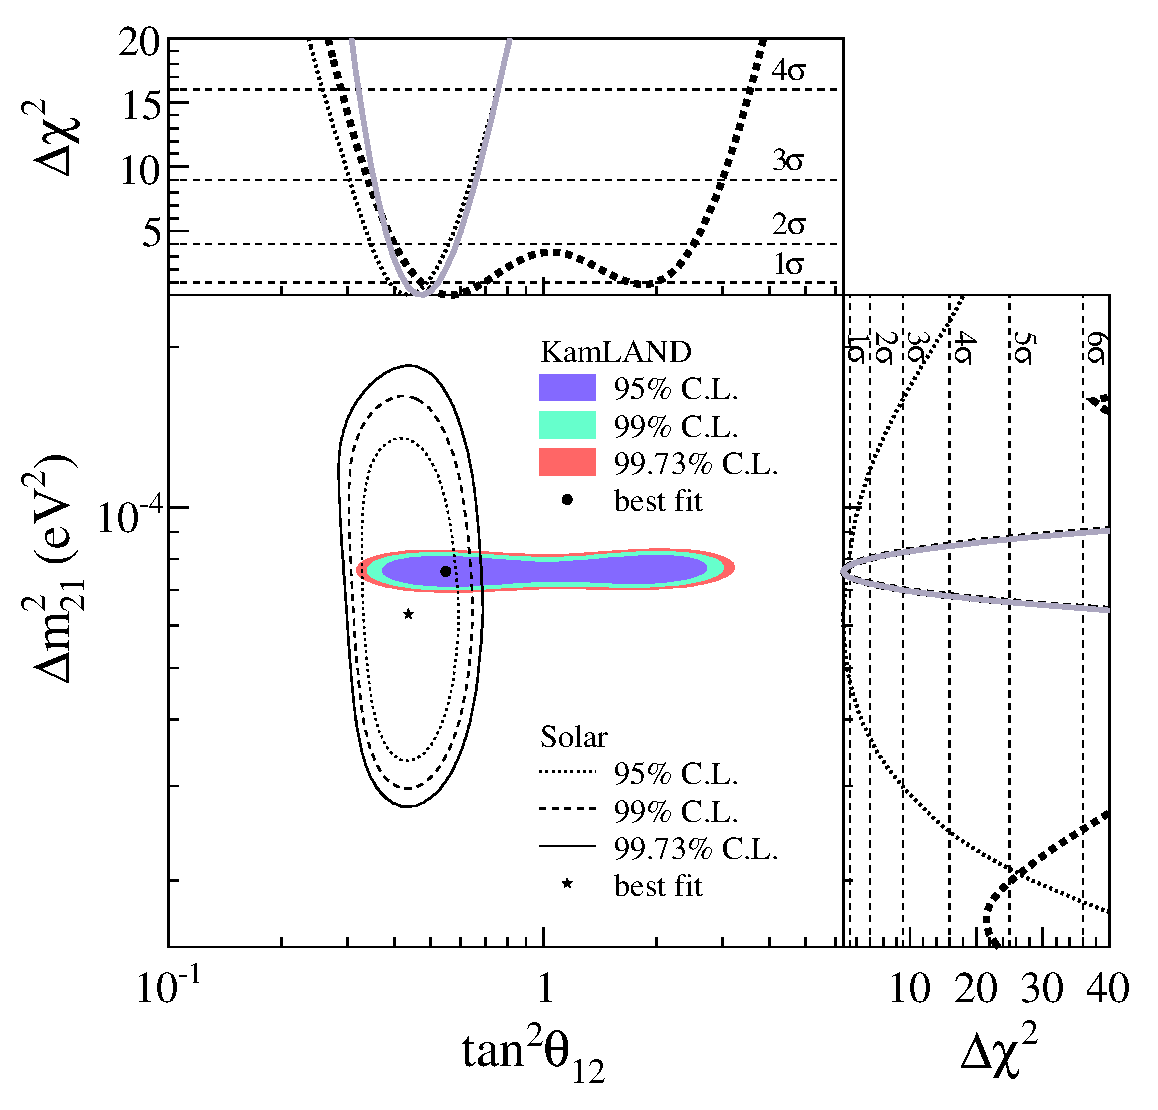
\includegraphics[width=0.7\textwidth]{ch_introduction/kamland_solar_fit}
    \caption[Solar oscillation parameters allowed region]{
        Allowed region for neutrino oscillation parameters from KamLAND and solar
        neutrino experiments.
        The side-panels show the $\Delta \chi^2$-profiles
        for KamLAND (dashed) and solar experiments (dotted) individually,
        as well as the combination of the two (solid).
        Figure and caption taken from \cite{kamland_latest}.
    }
    \label{fig:kamland_plus_solar}
\end{figure}

\subsubsection{Atmospheric parameters}
The Super-Kamiokande experiment measured $\theta_{23}$ and $\Delta m^2_{32}$
by comparing the rate of atmospheric neutrinos
traveling upward to those traveling downward
as described in \cref{subsec:atmospheric_anomaly}.
A nonzero up-down asymmetry of $-0.296\pm0.048(\text{stat.})\pm0.01(\text{syst.})$
was observed for muon-type events (including neutrinos and antineutrinos),
but the up-down asymmetry for electron-type events
of $-0.036\pm0.076\pm0.02$ was consistent with zero \cite{superk1998}.
Later investigations \cite{superk2004} showed the characteristic $L/E$
dependence when comparing the observed muon-type events
to a Monte Carlo prediction,
with the distance traveled inferred from the zenith angle
(see \cref{fig:superk_l_over_e}).
The events used in the analysis had $L/E$ values reconstructed
with a resolution of \SI{<70}{\percent},
thus the characteristic shape of the $L/E$ curve
was largely smeared out.
However, the location of the oscillation maximum
can be seen in \cref{fig:superk_l_over_e}
(where it takes the form of a survival minimum),
providing the first measurement of $\Delta m^2_{32} = \SI{2.4e-3}{\eV\squared}$
Equally importantly, the asymptotic behavior
at large $L/E$ revealed
the average value for the oscillation probability.
Since the average value was ${\sim}1/2$,
the observation favored a value of $\sin^22\theta_{23} = 1$,
corresponding to maximal mixing.

\begin{figure}
    \centering
    \includegraphics[width=0.5\textwidth]{ch_introduction/superk_atmo_l_over_e}
    \caption[Super-Kamiokande atmospheric L/E distribution]{
        Ratio of the data to the MC events without neutrino oscillation (points)
        as a function of the reconstructed L/E together with
        the best-fit expectation for 2-flavor $\nu_\mu\leftrightarrow\nu_\tau$
        oscillations (solid line).
        The error bars are statistical only.
        Also shown are the best-fit expectation for neutrino decay (dashed line)
        and neutrino decoherence (dotted line).
        Figure and caption taken from \cite{superk2004}.
    }
    \label{fig:superk_l_over_e}
\end{figure}

\subsubsection{Reactor parameter}
The measurement of the third mixing angle \thetaot{}
will be described in detail in \cref{sec:experiment_intro}.
This angle
governs the probability of $\nu_e$ (dis)appearance
at the atmospheric scale of $L/E \sim \SI{1}{\km\per\MeV}$
and is accessible by observing reactor \nuebar{} disappearance
and accelerator $\nu_e$ and \nuebar{} appearance.

\subsubsection{CP phase and mass ordering}
The final mixing parameter, $\delta_{CP}$,
is the subject of considerable current experimental effort.
Attempts to measure $\delta_{CP}$ involve
accelerator experiments comparing the rates of
$\nu_\mu\to\nu_e$ and $\bar{\nu}_\mu\to\bar{\nu}_e$ oscillations.
The current generation of experiments consists of
T2K, which utilizes the Super-Kamiokande detector,
and NOvA,
which uses a large segmented liquid scintillator detector \cite{nova_deltacp}.
The T2K experiment recently published evidence of $\delta_{CP}\neq 0$
at a significance of $3\sigma$ \cite{t2k_deltacp}.
These experiments provided the above-referenced measurement to $\delta_{CP}$
(\cref{eq:current_values}).
The next generation of experiments is currently under construction
and includes DUNE in the United States \cite{dune_potential}
and Hyper-Kamiokande in Japan \cite{hyperk2015}.

Two classes of experiments are sensitive to the neutrino mass ordering.
The first is the same accelerator experiments searching for $\delta_{CP}$;
the neutrino beams in these experiments travel substantial distances
through the Earth's crust,
which induces different distortions to the $\nu_e$ appearance spectrum
depending on the mass ordering.
The second class of experiments currently consists of
a single experiment under construction: JUNO \cite{junoproposal2016}.
Using similar technology to Daya Bay,
the JUNO experiment will perform a precise measurement
of the reactor \nuebar{} spectrum
at the $\Delta m^2_{21}$ oscillation maximum,
where the slight difference between
$\Delta m^2_{32}$ and $\Delta m^2_{31}$
will cause different effects depending
on which mass splitting is larger.
Current observations from accelerator experiments
have better agreement with normal ordering (NO)
predictions than with IO at the level of $2.4\sigma$ to $3.4\sigma$ \cite{pdg}.

\section{Reactor neutrino experiments and \texorpdfstring{\thetaot}{theta13}}
\label{sec:experiment_intro}

As illustrated by \cref{fig:oscprob},
the probability of a transition of $\nu_e \leftrightarrow \nu_\mu$
or $\nu_e \leftrightarrow \nu_\tau$
has two characteristic wavelengths and amplitudes:
the larger is governed by $\theta_{12}$ and $\Delta m^2_{21}$,
while the smaller is governed by
$\theta_{13}$, $\Delta m^2_{32}$, and $\Delta m^2_{31}$
with a typical $L/E$ scale of \SI{\sim0.5}{\km\per\MeV}.
The two experimentally-feasible signatures for \thetaot{}-governed oscillations
are $\nu_\mu\to\nu_e$ (appearance) and $\nu_e\to\nu_{\mu/\tau}$ (disappearance).
Appearance is most conveniently observed using accelerator neutrinos,
which are produced as a beam of primarily $\nu_\mu$ or $\bar{\nu}_\mu$.
Disappearance is easiest to observe using reactor \nuebar.

The survival probability for an electron (anti)neutrino
is given by applying \cref{eq:survival_prob_general}
to the PMNS matrix elements in \cref{eq:pmns}:
\begin{align}\label{eq:p_sur_ee}
    \begin{split}
        P_{e\to e} = 1 &-
        \sin^22\theta_{12}\cos^4\theta_{13}
        \sin^2\Delta_{21} \\
                       &-
        \sin^22\theta_{13}(\cos^2\theta_{12}
        \sin^2\Delta_{31}
                       +
        \sin^2\theta_{12}
        \sin^2\Delta_{32}
        ),
    \end{split}
\end{align}
where the oscillation phase $\Delta_{ij}$ is given by \cref{eq:osc_phase_shorthand}.
Note that this expression, like all survival probabilities by virtue of CPT symmetry,
is independent of $\delta_{CP}$.
At the $L/E\sim\SI{0.5}{\km\per\MeV}$ scale of reactor experiments,
$\Delta_{21} \sim 0.05$;
thus the impact from the first term in \cref{eq:p_sur_ee},
containing the the influence of the solar oscillation parameters,
is small, though not negligible.

The Daya Bay experiment is not sensitive
to the difference between $\Delta m^2_{32}$ and $\Delta m^2_{31}$,
so it is convenient to model the survival probability
using the approximation
\begin{equation}\label{eq:p_sur_dmee}
    P_{e\to e} \approx 1
    - \sin^22\theta_{12}\cos^4\theta_{13}\sin^2\Delta_{21}
    - \sin^22\theta_{13}\sin^2\Delta_{ee},
\end{equation}
where $\Delta_{ee}$ is defined in analogy to $\Delta_{ij}$
using the mass scale $\Delta m^2_{ee}$,
which is defined as the value which provides the best fit
of \cref{eq:p_sur_dmee} to observations.
This approximate model has been used to provide
model-independent measurements of the mass splittings
without relying on an assumption of the neutrino mass ordering
\cite{ngd2014,ngd2015,ngd2016,ngd2018}.
This thesis uses the exact three-flavor formula in \cref{eq:p_sur_ee}
assuming the normal ordering (NO),
so a detailed description of $\Delta m^2_{ee}$
will be left to the supplemental material of \cite{ngd2015}.
Given current measurements of the neutrino masses and mixing parameters,
$\Delta m^2_{ee}$ can be converted to $\Delta m^2_{31}$ and $\Delta m^2_{32}$
using the following relation:
\begin{align}\label{eq:dmee_conversion}
    \begin{split}
        \Delta m^2_{32} = \dmee - \SI{5.17e-5}{\eV\squared} \\
        \Delta m^2_{31} = \dmee - \SI{5.17e-5}{\eV\squared} + \Delta m^2_{21}.
    \end{split}
\end{align}

\subsection{Experimental principles for measuring \texorpdfstring{\thetaot}{theta13}}
\label{subsec:theta13_experiments}

Given that atmospheric neutrino observations were consistent
with a two-flavor oscillation model which only included $\nu_\mu\leftrightarrow\nu_\tau$,
it was inferred that any $\nu_\mu\leftrightarrow\nu_e$ transitions
at the atmospheric oscillation scale
must occur with low or zero probability.
The Chooz and Palo Verde reactor \nuebar{} experiments
attempted to observe the disappearance of \nuebar{} in the 1990s
\cite{chooz1999,paloverde2001};
the consistency of their observations with the predicted no-oscillation flux
provided constraints of $\sin^22\thetaot \lesssim 0.1$,
but were limited by systematic uncertainties
due to models of reactor \nuebar{} emission
and of detector response and detection efficiency.
\Cref{fig:chooz_exclusion} shows the best limits
from reactor and atmospheric measurements
based on the full Chooz data set.
Follow-up experiments were planned,
and attempts to measure \thetaot{} via $\nu_e$ appearance
using accelerator neutrinos were undertaken.

\begin{figure}
    \centering
    \includegraphics[height=0.6\textheight]{ch_introduction/chooz_exclusion}
    \caption[Constraint on \thetaot{} by Chooz]{
        Exclusion contours for $\sin^22\thetaot$ and $\Delta m^2_{32}$
        at the end of the Chooz experiment \cite{chooz1999}.
        The hashed regions represent the exclusion contours
        based on Super-Kamiokande atmospheric measurements.
    }
    \label{fig:chooz_exclusion}
\end{figure}


There are numerous systematic uncertainties associated with the $\nu_\mu\to\nu_e$ appearance measurement
which have until the last decade or so been prohibitive.
For example, since the probability of $\nu_e$ appearance is so small,
just a few percent,
the proportion of the beam that is either $\nu_\mu$ or $\nu_\tau$ is large,
necessitating extremely accurate flavor identification of detected events.
A small false positive rate of mistaking $\nu_\mu$ events as $\nu_e$
would substantially bias the measurement.
Further, the composition of the neutrino beam must be known extremely well.
The standard method for neutrino beam production (\cref{subsec:nu_flavors})
also produces charged kaons, which decay to $e^\pm + (\nu_e/\nuebar)$
with a much larger branching ratio than the equivalent decay for pions.
Thus a measurement of $\nu_e$ appearance must be able to justify
that it is not simply observing $\nu_e$ that were produced directly
by the accelerator.

On the other hand, the disappearance measurement using reactor \nuebar{} is
free from many of the issues faced by the accelerator experiments.
With characteristic energies of \SIrange{1}{8}{\MeV},
any antineutrinos which oscillated into $\bar{\nu}_{\mu/\tau}$
would be below threshold for producing the associated charged lepton,
obviating the need for flavor identification.
Further, nuclear reactors produce neutrinos via $\beta^-$ decay,
thus producing only \nuebar{}.
The ideal interaction to observe these \nuebar{} events
is inverse beta decay (IBD),
which was used by Reines and Cowan in the first detection of (anti)neutrino events,
not coincidentally also from reactor \nuebar{} (\cref{subsec:discovery}).
As in the Reines and Cowan experiment,
modern reactor \nuebar{} experiments use liquid scintillator
as a detection medium.
Unlike in that earlier experiment, though,
modern experiments use liquid scintillator as the antineutrino target itself,
using organic scintillators with a large number of free protons
in the form of \isotope[1]{H}.
Systematic uncertainties arise in constraining the reactor \nuebar{} flux,
characterizing the detector response,
and in accumulating sufficient statistics
so that any observed deficit of \nuebar{}
can be attributed to \thetaot{} rather than to mis-modeling of the reactor
or detector or to a statistical fluctuation.

A new generation of reactor experiments
was designed to remedy the issue of reactor systematics
by constructing antineutrino detectors at both near and far sites
with respect to the reactor cores,
with the near detectors constraining the \nuebar{} flux prediction
and decreasing the systematic uncertainty \cite{near_far_proposal}.
The value of $\theta_{13}$ was first measured
with a significance of $\geq 5\sigma$
by the Daya Bay experiment in April 2012 \cite{ngd2012},
followed closely by the RENO \cite{reno2012}
and Double Chooz \cite{doublechooz2012} experiments.
Accelerator experiments T2K and MINOS
searched for $\nu_\mu\to\nu_e$ ($\nu_e$ appearance)
and observed evidence for a nonzero \thetaot{}
as early as 2011 \cite{t2k2011,minos2011},
but only at a significance of $2\sigma$ to $3\sigma$.
Subsequent searches by accelerator experiments (e.g. \cite{t2k2018})
resulted in values of \thetaot{} which generally agree
with the reactor measurements.

Since the start of data taking on 24 December 2011,
the Daya Bay Reactor Neutrino Experiment has produced numerous measurements of
\thetaot{}, searches for sterile neutrinos \cite{dyb_sterile2020},
and the reactor \nuebar{} flux and spectrum \cite{dyb_spec_decomp2019},
and has also investigated
a variety of other physical phenomena (e.g. \cite{dyb_cpt2018}).
The April 2012 measurement of \thetaot{} used 55 days of \nuebar{} data
and only six of the eight planned antineutrino detectors.
Since then, Daya Bay has published updated results using IBDs detected by
either neutron capture on gadolinium (nGd)
\cite{ngd2012,ngd2013,ngd2014,ngd2015,ngd2016,ngd2018}
or neutron capture on hydrogen (nH)
\cite{nh2014,nh2016}
as shown in \cref{fig:theta13_vs_t}.

\begin{figure}
    \centering
    \includegraphics[width=0.9\textwidth]{ch_introduction/theta13_vs_time_existing}
    \caption[Daya Bay \thetaot{} results over time]{
        Published values of $\sin^{2}2\thetaot$ over time
        for both nGd and nH analyses by the Daya Bay experiment.
        Some nGd results were reported with separate statistical
        and systematic errors;
        those have been combined linearly for this plot.
    }
    \label{fig:theta13_vs_t}
\end{figure}

This thesis will present a new measurement of \thetaot{}
based on observation of nH-IBD interactions
at the Daya Bay experiment,
with a focus on potential sources of the ${\sim}1\sigma$ discrepancy
between the nGd and nH extracted values for \thetaot{}.
The Daya Bay detector system is described in \cref{ch:detector}.
Calibration procedures and event reconstruction algorithms
are described in \cref{ch:calibration,ch:reconstruction}, respectively.
The procedure for selecting nH-IBD events and rejecting backgrounds
is described in \cref{ch:event_selection}.
In \cref{ch:simulation}, details of Monte Carlo simulation studies
will be presented.
\Cref{ch:analysis} will present the extraction of \thetaot{}
from the selected events.


\chapter{The Daya Bay Reactor Antineutrino Experiment}
\label{ch:detector}

The Daya Bay Reactor Antineutrino Experiment was designed
to be sensitive to $\thetaot \sim 0.01$
by performing a relative measurement of the rate of \nuebar{}
using a modular detector system arranged at near and far sites \cite{dybproposal2006}.
The experiment was located in southeast China,
approximately \SI{55}{\km} northeast of Hong Kong,
on the campus of the Daya Bay and Ling Ao Nuclear Power Plants.
Groundbreaking for civil construction of the three underground
experimental halls occurred in October 2007,
and construction lasted approximately 4 years \cite{dyb_overview}.
The antineutrino detectors in the first experimental hall (EH1)
were ready for data taking on 11 August 2011,
and EH2 was ready on 5 November 2011.
With the completion of EH3, data taking began on 24 December 2011
and, with only brief interruptions,
continued until 12 December 2020.

The Daya Bay site is ideal for an oscillation experiment.
Its six reactor cores together form one of the most intense \nuebar{}
sources on Earth \cite{detector_system}.
The power plant campus is also located at the base of a mountain ridge,
providing an ideal location for antineutrino detectors that must be
protected from cosmic-ray muons without having to dig deep mines.
The tunnel layout allowed for easy access to the experiment via electric golf cart.

\section{Reactors and experimental halls}

Six pressurized-water nuclear reactors were used
as the \nuebar{} source for Daya Bay.
Each reactor had an output of \SI{2.9}{\giga\watt_{th}}
and combined they produced approximately \num{3.5e21}\,\nuebar/s \cite{ngd2016}.
The reactors are arranged in three pairs: Daya Bay, Ling Ao, and Ling Ao II.
The location of the cores determined the layout of the Daya Bay experiment.

The experiment was arranged into three experimental halls (EHs).
EH1 was located close to the Daya Bay cores (\SIrange{357}{372}{\meter}),
and EH2 was located close to the Ling Ao and Ling Ao II cores
(\SIrange{467}{558}{\meter}).
They are therefore known collectively as the near halls.
Their purpose was to constrain the \nuebar{} flux for the
relative oscillation measurement,
and they each contained two antineutrino detector modules (ADs).
EH3 was located farther away, approximately \SI{2}{\km} from the Daya Bay cores
and \SI{1.5}{\km} from the Ling Ao cores,
and was correspondingly called the far hall.
EH3 was located at the first oscillation minimum
for the oscillation controlled by $\Delta m^2_{32}$ (and $\Delta m^2_{31}$)
and its purpose was to measure the decrease in \nuebar{} rate compared to the near halls.
To increase statistics, EH3 contained four ADs.
The layout of the EHs with respect to the reactors is shown in \cref{fig:layout}.
The positions of the ADs and reactor cores were measured using
two independent surveying procedures: GPS for the above-ground locations
(reactor cores and tunnel entrances),
and a total station survey,
which was able to replicate the GPS survey to within \SI{4}{\mm}
and extend the surveyed area underground into the tunnels and EHs.
The baselines from each reactor to each AD are listed in \cref{tab:baselines}.
An uncertainty for each baseline of less than \SI{18}{\mm}
was assessed to have negligible impact on the oscillation measurement
\cite{detector_system}.

\begin{figure}
    \centering
    \begin{subfigure}{0.49\textwidth}
        \includegraphics[width=\textwidth]{ch_detector/dayabay_map}
    \end{subfigure}
    \begin{subfigure}{0.49\textwidth}
        \includegraphics[width=\textwidth]{ch_detector/dayabay_map_3d}
    \end{subfigure}
    \caption[Daya Bay geographic layout]{Two views of the layout of the Daya Bay experiment.}
    \label{fig:layout}
\end{figure}

The EHs were located underneath a mountain, which provided a substantial
overburden to protect against cosmic-ray muons:
\SIlist{250;265;860}{\mwe} (meters of water equivalent),
respectively, for EH1, EH2 and EH3.

\begin{table}[ht]
    \centering
    \begin{tabular}[t]{lSSSSSSS}
        \toprule
        & {D1} & {D2} & {L1} & {L2} & {L3} & {L4} \\
        Detector & \multicolumn{6}{c}{Baseline [m]} \\
        \midrule
        EH1-AD1 & 362.38 & 371.76 & 903.47 & 817.16 & 1353.62 & 1265.32 \\
        EH1-AD2 & 357.94 & 368.41 & 903.35 & 816.90 & 1354.23 & 1265.89 \\
        EH2-AD1 & 1332.48 & 1362.88 & 472.97 & 489.58 & 557.58 & 499.21 \\
        EH2-AD2 & 1337.43 & 1362.88 & 472.97 & 495.35 & 558.71 & 501.07 \\
        EH3-AD1 & 1919.63 & 1894.34 & 1533.18 & 1533.63 & 1551.18 & 1524.94 \\
        EH3-AD2 & 1917.52 & 1891.98 & 1534.92 & 1535.03 & 1554.77 & 1528.05 \\
        EH3-AD3 & 1925.26 & 1899.86 & 1538.93 & 1539.47 & 1556.34 & 1530.08 \\
        EH3-AD4 & 1923.15 & 1897.51 & 1540.67 & 1540.87 & 1559.72 & 1533.18 \\
        \bottomrule
    \end{tabular}
    \caption[Reactor-AD baselines]{Reactor-to-AD baselines \cite{ngd2016}.}
    \label{tab:baselines}
\end{table}

To accelerate the experiment startup timeline,
only six of the planned eight ADs were installed in 2011:
2 in EH1, 1 in EH2, and 3 in EH3.
This so-called 6-AD period lasted from 24 December 2011 until 28 July 2012.
The experiment was shut down while the remaining two ADs were installed
in EH2 and EH3.
The 8-AD period began on 19 October 2012.
At the end of 2016, EH1-AD1 was chosen to be repurposed as a test stand
for liquid scintillator studies for the JUNO experiment \cite{junoproposal2016},
and was decommissioned from Daya Bay on 20 December 2016.
The 7-AD period began on 26 January 2017 and continued through the end of
the Daya Bay experiment on 12 December 2020.

The ADs within each hall were collectively surrounded by a water pool,
which acted as a passive shield against natural radioactivity present in the rock
as well as an active veto for muons which penetrate through the overburden.
The water pool was covered by a resistive plate chamber (RPC) array
to provide additional sensitivity to incoming muons.
\Cref{fig:eh3_wp_photo} shows a photograph of EH3 during installation of the ADs,
when the RPC had not yet been moved into position to cover the water pool.
Also visible mounted to the near and far walls are two muon RPC telescopes
which were used for muon studies during detector commissioning \cite{muonsystem2015}.

\begin{figure}
    \centering
    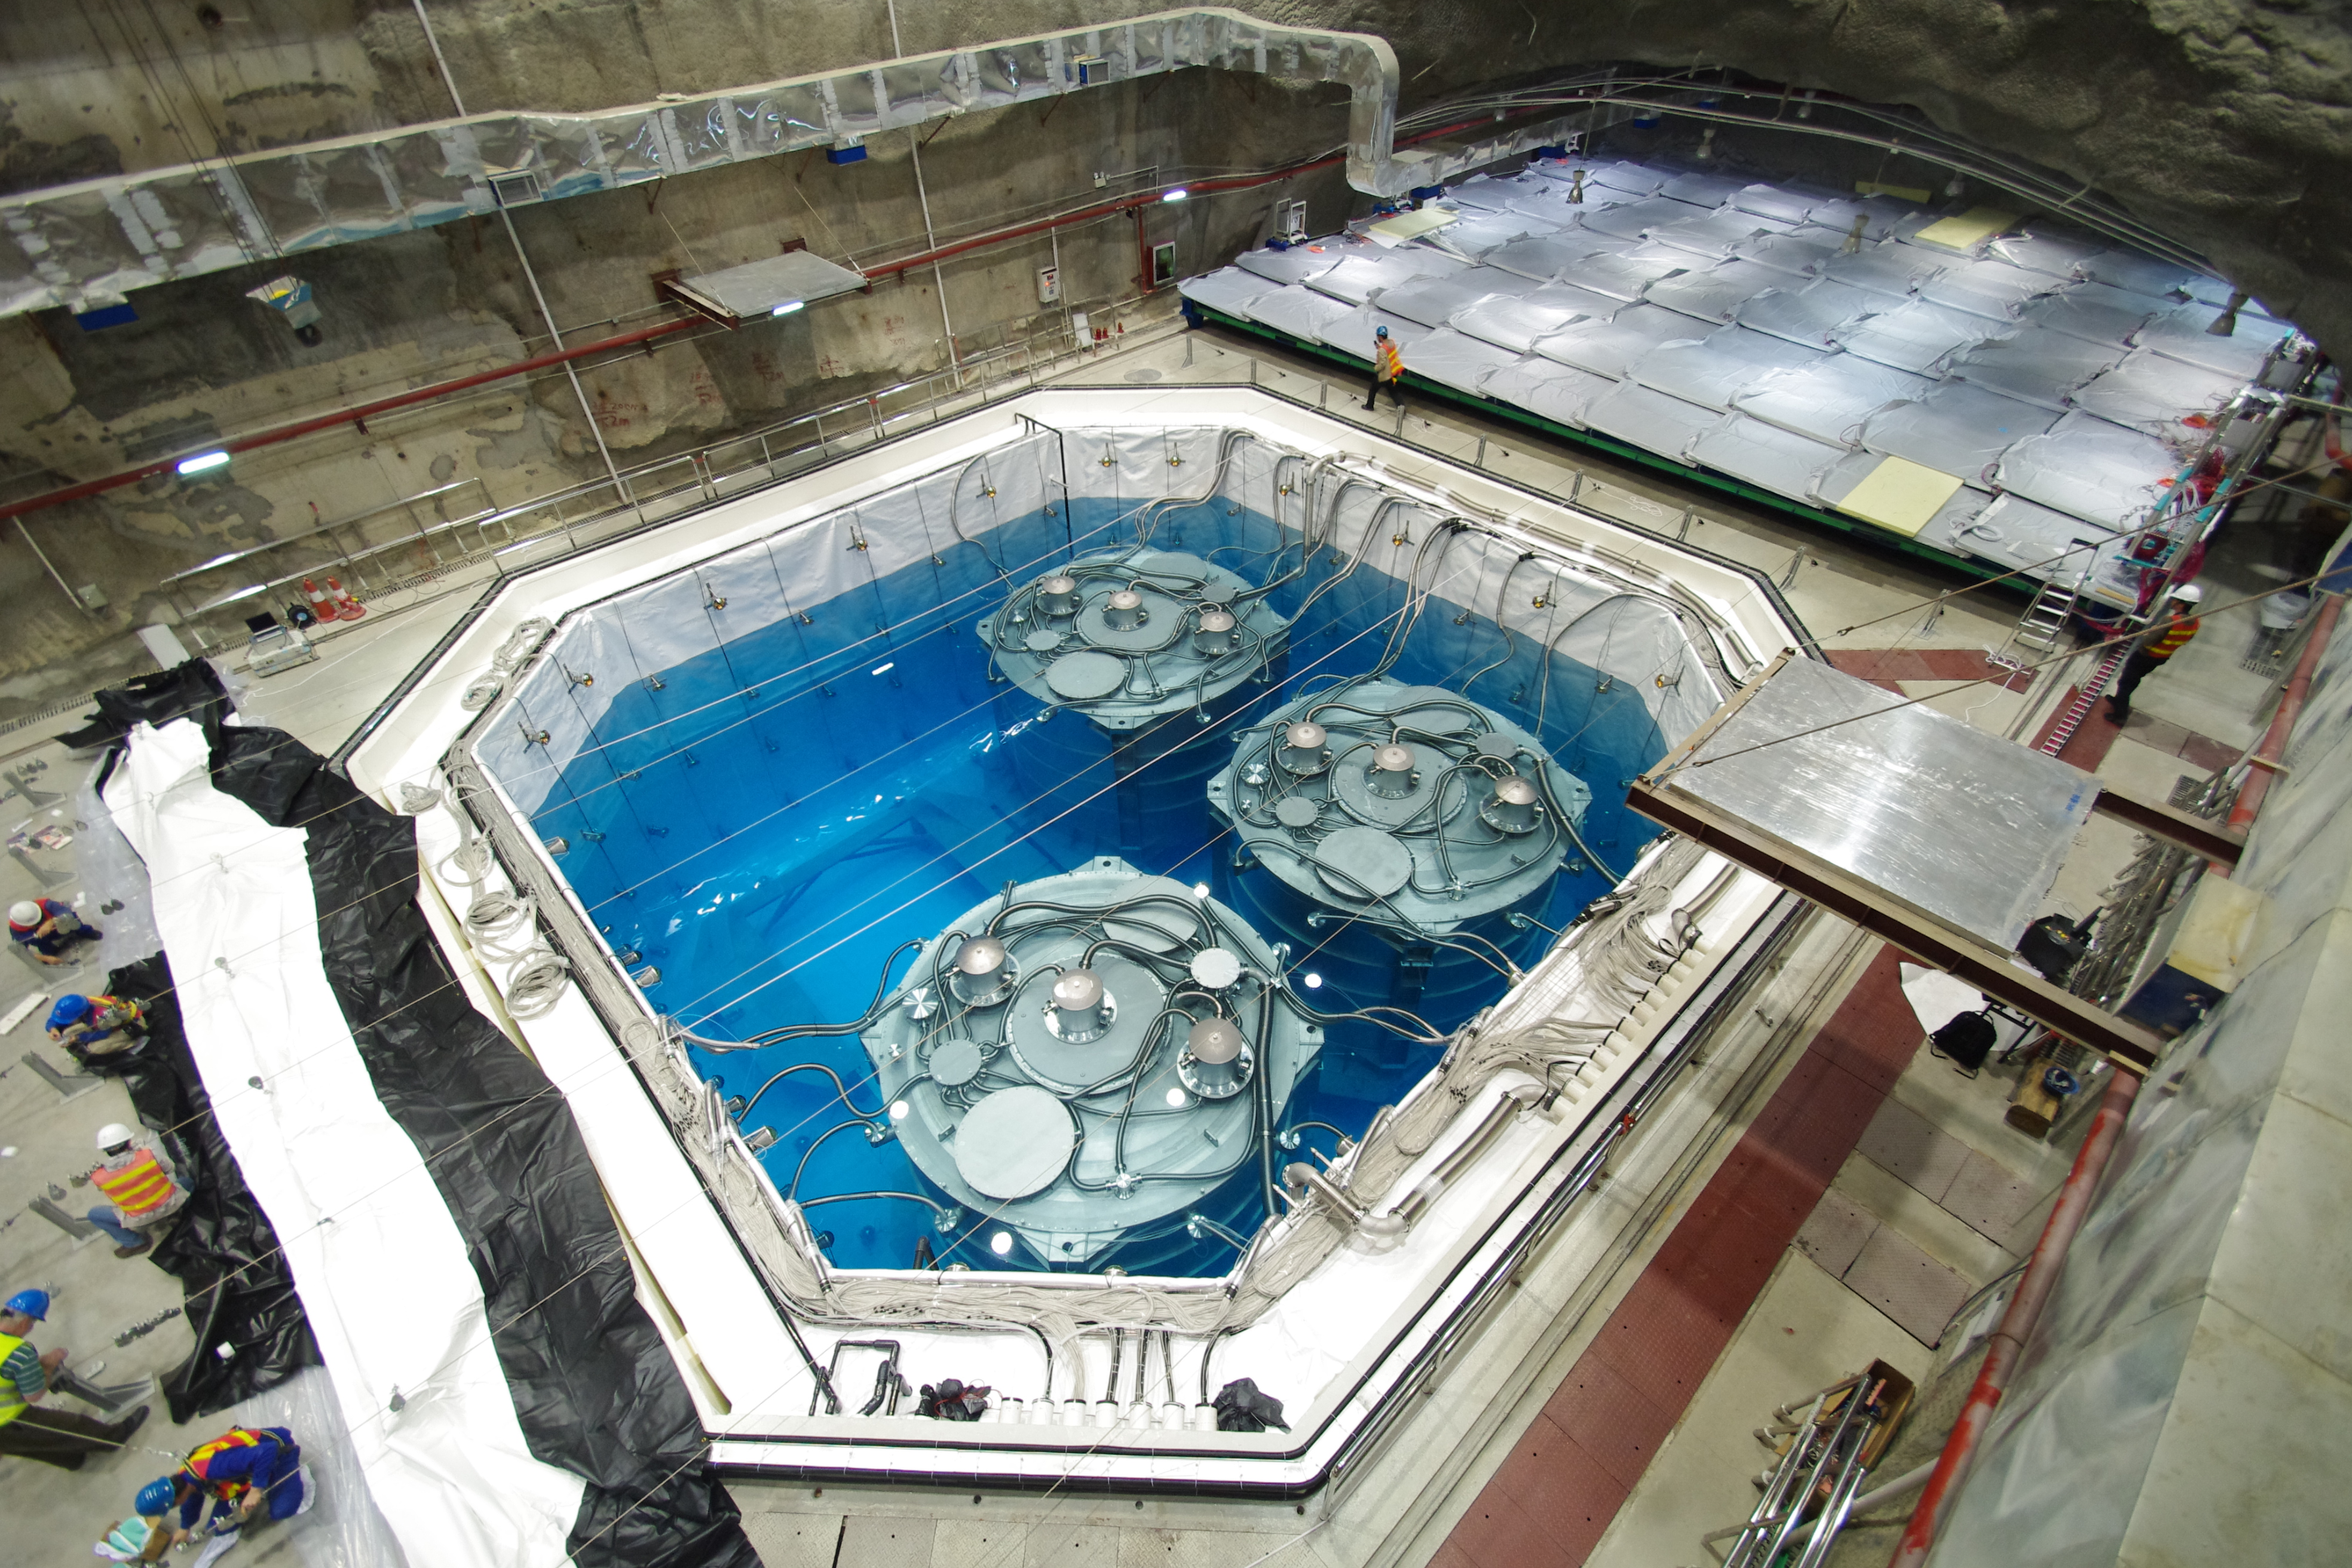
\includegraphics[width=0.5\textwidth]{ch_detector/EH3_installation_6ADperiod}
    \caption[View of EH3]{EH3 during the installation of the first three ADs.}
    \label{fig:eh3_wp_photo}
\end{figure}

\section{Antineutrino detectors}

The eight antineutrino detectors (ADs) were used to measure
the rate and energy of millions of \nuebar{} interactions with high precision
and low systematic uncertainty.
Each AD consisted of three concentric cylindrical regions
contained in an outer stainless steel vessel (SSV),
a cylinder with diameter and height of \SI{5}{\m}.
The innermost region was filled with \SI{0.1}{\percent} by mass
Gadolinium-doped liquid scintillator (GdLS).
The GdLS was contained by an acrylic cylinder known as the inner acrylic vessel (IAV).
The middle region between the IAV and the outer acrylic vessel (OAV) was filled
with (plain, undoped) liquid scintillator (LS).
The outer region between the OAV and SSV was filled with mineral oil
that served as a final passive layer of shielding around the LS region.

Two views of the nested AD configuration are shown in \cref{fig:ad_cutaway}.
The IAVs had a height and diameter of \SI{3}{\m} and were filled with \SI{20}{\tonne}
of GdLS.
The OAVs had a height and diameter of \SI{4}{\m} and were filled with \SI{20}{\tonne}
of LS.
The SSVs had a height and diameter of \SI{5}{\m} and were filled with \SI{40}{\tonne}
of mineral oil.
Each acrylic vessel was made of UV-transparent acrylic
and had a thickness of approximately \SI{1.5}{\cm}.

The liquid scintillator cocktail was designed to optimize the optical properties
and maximize stability over time \cite{gdls2014}.
Linear alkylbenzene (LAB) was used as the solvent and \nuebar{} target,
into which \SI{3}{\g\per\liter} of 2,5-diphenyloxazole (PPO)
was dissolved as a fluor,
along with \SI{15}{\mg\per\liter} of the wavelength shifter
p-bis-(o-methylstyryl)-benzene (bis-MSB).
This LS was used to fill the OAV.
To dissolve Gd into the LS to fill the IAV, the chelating ligand
3,5,5-trimethylhexanoic acid (TMHA) was chosen for its ease of production
and its stability in solution with LAB.
During LS production, the approximately \SI{185}{\tonne} of GdLS for the IAV
was produced first,
after which the equipment was cleaned with a diluted HCl solution and purified water
so that the undoped LS could then be produced for the OAV.

Each AD contained overflow tanks to allow the liquid in each region
to respond to the slight expected changes in temperature and pressure.
ADs were also fitted with three automated calibration units (ACUs)
which contained radioactive sources and LEDs to help calibrate the ADs.
The ACUs are described in detail in \cref{ch:calibration}.

The mineral oil region contained the 192 8-inch Hamamatsu R5912
photomultiplier tubes (PMTs) that monitored the AD for scintillation light
(and, secondarily, Cherenkov radiation).
The PMTs were arranged in 8 rings of 24 PMTs on the outer edge of the mineral oil region.
Light collection and detector uniformity was increased by the presence of
specular reflectors located on the top and bottom faces of the OAV,
as indicated in \cref{fig:ad_cutaway}.
PMTs consist of a sensitive photocathode, from which an incident photon
can eject an electron by the photoelectric effect.
The photoelectron (PE) is accelerated in an electric field to the first dynode,
a charged metal plate, where it causes multiple electrons to be ejected.
A series of subsequent dynodes leads to an avalanche effect of electrons,
which are collected at the anode and read out as a voltage signal.
When discussing the strength of a PMT signal,
it is customary to use the term ``charge'' (measured in PE)
rather than ``light,''
though the charge collected by a PMT anode
is of course a proxy for the number of incident photons.

Before the ADs were filled with LS, GdLS, and mineral oil,
they were tested in a series of so-called dry runs \cite{dryrun1}.
The PMTs were supplied with high voltage
to verify the stability of the gain and dark rate.
The ACUs were deployed, and the calibration LEDs
were used to induce charge signals on the PMTs
to exercise not only the PMTs but also the front-end electronics,
the online DAQ system and the offline storage.
It was during the dry runs that the issue of PMT light emission,
or flasher events, was discovered.
These events must be filtered out from the data stream,
as described in \cref{sec:flashers}.

\begin{figure}
    \centering
    \begin{subfigure}{\textwidth}
        \centering
        \includegraphics[height=0.4\textheight]{ch_detector/ADcutaway_2D}
    \end{subfigure}
    \vspace{1cm}\\
    \begin{subfigure}[0.4\textheight]{\textwidth}
        \centering
        \includegraphics[height=0.4\textheight]{ch_detector/ADcutaway}
    \end{subfigure}
    \caption[Layout of a Daya Bay AD]{
        Two views of the Daya Bay antineutrino detector (AD)
        \cite{ngd2016,internal_files}.
        The coordinate system origin is in the center of the GdLS region,
        as indicated by the star symbol in the 2D view.
        Positive $z$ is upwards.
    }
    \label{fig:ad_cutaway}
\end{figure}

\subsection{Target protons}
\label{subsec:target_mass}

The number of target protons in each AD must be measured precisely;
a mis-characterization would lead to an unexplained excess or deficit
in event counts which could bias the measurement of \thetaot{}
in the same manner as a variation in detection efficiency.
Thus the number of target protons was treated as an effective efficiency
\begin{equation}\label{eq:target_protons_eff}
    \varepsilon_{\text{p},i} = \frac{N_{\text{p,\,AD }i}}{N_\text{p,\,EH1-AD1}}.
\end{equation}
When measurements from different ADs were compared,
the event rates were corrected by $\varepsilon_{\text{p},i}$,
which had the effect of standardizing to the number of target protons in EH1-AD1.

The number of target protons for each AD was computed from the measured masses
of each target volume
and chemical analyses of the proton mass fractions
of the materials in each volume.
The volumes were divided into GdLS, LS, and other,
which was dominated by the acrylic vessels (IAV and OAV)
but also included the reflector, hold-downs and radial shield \cite{acrylic_mass}.
Target masses for each AD are listed in \cref{tab:target_masses}.
The proton density in each detector volume
was computed based on the analytically-computed
hydrogen mass fractions of LS, GdLS and acrylic \cite{target_protons_technote}.
The final number of target protons was
simply the product of the target mass and the proton density,
summed over detector volumes:
\begin{equation}\label{eq:target_protons}
    N_\text{p} = m_\text{GdLS} n_\text{p,\,GdLS}
    + m_\text{LS} n_\text{p,\,LS}
    + m_\text{other} n_\text{p,\,other}.
\end{equation}
The number of target protons for each AD
is listed in \cref{tab:target_protons}.
The uncertainty is dominated by the uncertainty of the LS mass;
the relative uncertainty of \SI{0.37}{\percent}
is a sub-dominant contribution to the AD-uncorrelated
relative efficiency uncertainty
as listed in \cref{tab:efficiency_summary}.


\begin{table}[ht]
    \centering
    \begin{tabular}[t]{
        l
        S[
            table-number-alignment=center,
            table-figures-integer=5,
            table-figures-decimal=0,
            separate-uncertainty,
            table-figures-uncertainty=2]
        S[
            table-number-alignment=center,
            table-figures-integer=5,
            table-figures-decimal=1,
            separate-uncertainty,
            table-figures-uncertainty=3
        ]
        S[
            table-number-alignment=center,
            table-figures-integer=4,
            table-figures-decimal=0,
            separate-uncertainty,
            table-figures-uncertainty=2
        ]
    }
        \toprule
         & {GdLS [\si{\kg}]} & {LS [\si{\kg}]} & {Other [\si{\kg}]}\\
        \midrule
        EH1-AD1 & 19941\pm5 & 21573.5\pm28 & 3697\pm18 \\
        EH1-AD2 & 19967\pm5 & 21519.6\pm28 & 3731\pm19 \\
        EH2-AD1 & 19891\pm5 & 21587.2\pm28 & 3664\pm18 \\
        EH2-AD2 & 19944\pm5 & 21449.9\pm28 & 3749\pm19 \\
        EH3-AD1 & 19917\pm5 & 21566.2\pm28 & 3744\pm19 \\
        EH3-AD2 & 19989\pm5 & 21408.8\pm28 & 3864\pm19 \\
        EH3-AD3 & 19892\pm5 & 21652.6\pm28 & 3844\pm19 \\
        EH3-AD4 & 19931\pm5 & 21474.5\pm28 & 3794\pm19 \\
        \bottomrule
    \end{tabular}
    \caption[Target masses for each AD volume]{
        Target masses for each AD volume from
        \cite{liquid_target_mass,nh2016technote,detector_system}.
    }
    \label{tab:target_masses}
\end{table}

\begin{table}[ht]
    \centering
    \begin{tabular}[t]{
            l
            S[
                table-number-alignment=center,
                table-figures-integer=3,
                table-figures-decimal=2,
                separate-uncertainty,
                table-figures-uncertainty=3
            ]
        }
        \toprule
        & {$N_\text{p}$ [$\times10^{28}$]} \ML
        EH1-AD1 & 314.14(117) \NN
        EH1-AD2 & 314.11(117) \NN
        EH2-AD1 & 313.72(117) \NN
        EH2-AD2 & 313.53(117) \NN
        EH3-AD1 & 314.15(117) \NN
        EH3-AD2 & 314.12(117) \NN
        EH3-AD3 & 315.10(117) \NN
        EH3-AD4 & 313.83(117)
        \LL
    \end{tabular}
    \caption[Number of target protons for each AD]{Number of target protons for each AD.}
    \label{tab:target_protons}
\end{table}

\subsection{Observing Inverse Beta Decay}
\label{subsec:ibd_intro}

The IBD reaction, $\nuebar + p \to e^+ + n$,
created two signals with a characteristic
time delay between them, in a pattern known as a ``double''
or ``delayed'' coincidence.
When this reaction occurred in either the GdLS or LS region
of a Daya Bay AD,
the positron quickly deposited its kinetic energy in the liquid scintillator
and annihilated within $\lesssim\SI{1}{\nano\second}$
into two \SI{0.511}{\MeV} $\gamma$-rays
which also deposited their energy into the scintillator.
The combined light from the kinetic energy and annihilation $\gamma$-rays
was the prompt signal
and served as an effective timestamp for the interaction
as well as a proxy for the energy of the incident \nuebar{}.
The total prompt energy was related to the incident antineutrino energy
via the mass-energy conservation relation
\begin{equation}\label{eq:prompt_vs_nu_energy}
    E_p \approx E_\nu - \delta m_{pn} + m_e \approx E_\nu - \SI{0.78}{\MeV},
\end{equation}
where $\delta m_{pn}$ is the mass difference between the neutron and proton.
Meanwhile, the neutron produced by IBD thermalized in the liquid scintillator
and captured on Gd (in the GdLS only) or on a proton in the form of \isotope[1]{H}
(in both the GdLS and LS).
This happened with a characteristic time of $\sim \SI{28}{\micro\second}$
in GdLS and $\sim \SI{215}{\micro\second}$ in LS.
The shorter time in the GdLS was by design,
due to the large capture cross section of a thermalized neutron
on a Gd nucleus compared to H (\SI{49}{\kilo\barn} vs. \SI{0.332}{\barn})
\cite{gdls2014}.
The term nGd is used to refer to the process of neutron capture on Gd
and the analysis of the data set containing nGd captures.
The analogue for neutron capture on H is nH.
For nGd captures, the excited nucleus
emitted $\gamma$-rays in one of two decay chains,
both of which had a combined energy of approximately \SI{8}{\MeV}.
The nH capture reaction $n+\isotope[1]{H} \to \isotope[2]{H} + \gamma$
produced a single \SI{2.2}{\MeV} $\gamma$-ray.
In either scenario, the $\gamma$-ray(s) deposited their energy
in the liquid scintillator.
The \SIlist[list-pair-separator = { or }]{8;2.2}{\MeV} signal
from the neutron capture on Gd or H, respectively, comprised the delayed signal of the
double coincidence.
This prompt-delayed coincidence pattern was an extremely efficient
discriminator for IBD events against a wide variety of sources of background.
The full IBD interaction and detection process
is depicted in \cref{fig:ibd_cartoon}.

\begin{figure}
    \centering
    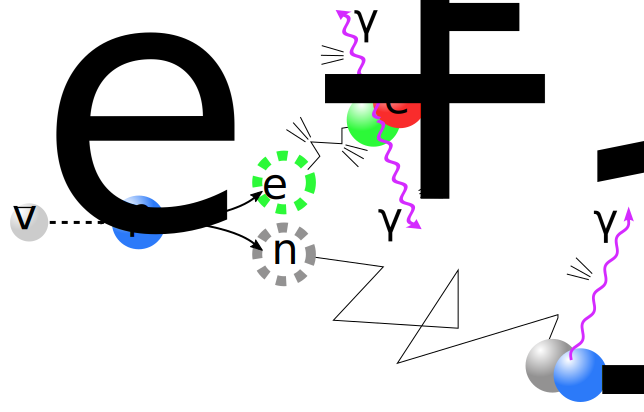
\includegraphics[width=0.8\textwidth]{ch_detector/ibd}
    \caption[Inverse Beta Decay diagram]{
        Graphical depiction of the IBD interaction and delayed coincidence
        for neutron capture on hydrogen (nH).
        The dotted outlined $e^+$ and $n$ represent the initial interaction products.
        The thin black lines represent their trajectories
        through the liquid scintillator.
        The ``whisker'' marks indicate production of scintillation light.
    }
    \label{fig:ibd_cartoon}
\end{figure}

The LS region served an important purpose for the main nGd \thetaot{} analysis.
It significantly reduced the fraction of $\gamma$-rays from nGd capture
that escaped from the scintillating volume and distorted the energy spectrum.
The presence of the LS region allowed the entire GdLS volume to be
the fiducial volume, obviating the need to cut on the reconstructed position
of events, which would have added additional uncertainties to the analysis.
However, for the nH analysis,
a $\gamma$-ray produced by nH capture in the LS region
had a higher likelihood of escaping.
This risk was somewhat mitigated by the lower energy of the nH $\gamma$'s
(\SI{2.2}{\mev} vs. \SI{8}{\mev}).
The nH \thetaot{} analysis in this thesis accounts for escaping $\gamma$'s
through assessment of the delayed energy cut efficiency (\cref{subsec:delayed}).


\section{Water pools and muon detectors}
\label{sec:wp}

The muon detection system for Daya Bay consisted of
the water pool and the RPC system covering the water pool.
As data from the RPC is not used in the \thetaot{} analysis,
its description, along with extensive details of the entire muon system,
will be left to \cite{muonsystem2015}.
All three water pools were \SI{10}{\m} deep.
The near-hall water pools were \SI{10}{\m} wide and \SI{16}{\m} long,
while the far-hall water pool was \SI{16}{\m} in both dimensions.
These dimensions allowed the water pools to provide at least \SI{2.5}{\m} of shielding
to the ADs in every direction.
A cutaway diagram of the near-site water pools is shown in \cref{fig:wpcutout}.
Each water pool was divided using Tyvek(R) sheets
into optically-isolated inner and outer regions,
known as the inner water shield (IWS) and outer water shield (OWS).
Both the inner and outer water shields were instrumented with photomultiplier tubes (PMTs)
to detect the Cherenkov radiation from muons traversing the water.
The near-hall water pools each contained \num{288} PMTs,
and the far-hall water pools contained \num{384} PMTs.
A further breakdown is shown in \cref{tab:wp_pmts}.
\num{619} of these PMTs were newly-purchased \SI{20}{\cm}
model R5912 from Hamamatsu,
and the remaining \num{341} were \SI{8}{\inch} models 9350KA
and D642KB from EMI
donated by the MACRO experiment.
The IWS has been demonstrated to tag \SI{100}{\percent} of muons
that reach the ADs using the trigger thresholds described in \cref{tab:trigger}.


\begin{table}[ht]
    \centering
    \begin{tabular}[t]{llll}
        \toprule
        Hall & IWS & OWS (inward/outward) & Total\\
        \midrule
        EH1 & 121 & 167 (103/64) & 288\\
        EH2 & 121 & 167 (103/64) & 288\\
        EH3 & 160 & 224 (128/96) & 384\\
        \bottomrule
    \end{tabular}
    \caption[Muon system PMTs]{Muon system PMTs \cite{muonsystem2015}}
    \label{tab:wp_pmts}
\end{table}

\begin{figure}
    \centering
    \includegraphics[height=0.4\textheight]{ch_detector/nearSiteDiagram}
    \caption[Water pool and AD layout]{
        Water pool and AD layout in the near halls EH1 and EH2
        \cite{sidebyside}.
    }
    \label{fig:wpcutout}
\end{figure}



\section{Triggers and data acquisition}
\label{sec:daq}

Each Daya Bay AD PMT had a dedicated high-voltage (HV) coaxial cable
that supplied power to the PMT and returned the PMT signal to the
front-end electronics.
Upon receipt of an above-threshold PMT signal, these electronics immediately
issued a ``start'' signal to a TDC with \SI{1.6}{\ns} resolution,
and also measured the charge using a \SI{40}{\MHz} \num{12}-bit ADC
providing better than \num{0.1}-photoelectron (PE) resolution.
A \SI{50}{\percent} attenuated copy of the signal was passed to a copy
of the same ADC to allow for higher dynamic range in processing high-energy
events.
Refer to \cite{sidebyside,ngd2016} for the details
of the front-end electronics system.
The threshold to activate a single PMT channel's front-end electronics
was approximately \SI{0.25}{\pe}.
Once a channel was activated, the ADC values were buffered
awaiting a full-detector trigger signal.

The various detectors in an EH were triggered independently
by a master trigger board based on the conditions given in \cref{tab:trigger}.
The primary triggers for detecting \nuebar{}'s in the ADs were the NHIT and ESUM triggers.
The NHIT trigger was based on the number of PMTs simultaneously over threshold,
and the ESUM trigger was based on a simple sum of the photoelectrons
from each PMT.
The efficienies of the NHIT and ESUM triggers are shown in \cref{fig:trig_eff}.
Note that the trigger criteria are lower than the event selection
criteria used for the \thetaot{} analysis and described in \cref{ch:event_selection}.
Each channel's TDC was sent a ``stop'' signal when it received a trigger signal
from the master trigger board.
For every channel with a TDC reading of \SI{<1.2}{\us},
the corresponding TDC reading, peak ADC value and the pedestal ADC value
(the ADC output given no PMT signal)
were recorded into the offline storage system.
The absolute timestamp of the event was determined by a GPS-based clock
with \SI{25}{\ns} resolution and was also stored.
The resulting data files comprise the raw data from Daya Bay.


\begin{table}[ht]
    \centering
    \begin{tabular}[t]{lllp{6cm}}
        \toprule
        Detector & Criterion & Threshold value ($\geq$) & Explanation\\
        \midrule
        AD & NHIT & \num{45} & Number of PMTs over threshold \\
        AD & ESUM & $\SI{65}{\pe}\approx \SI{0.4}{\MeV}$ & Analog sum of signals \\
        IWS & NHIT & \num{6} & \\
        OWS (near-hall) & NHIT & \num{7} & \\
        OWS (far-hall) & NHIT & \num{8} & \\
        AD & CALIB & - & Calibration trigger simultaneous with LED flash \\
        \midrule
        \multicolumn{4}{c}{Ignored in \thetaot{} analysis} \\
        \cmidrule(r{17em}l{17em}){1-4}
        RPC & NHIT & \num{3} & Number of layers over threshold in a single module \\
        AD & RANDOM & - & Random triggers issued at \SI{10}{\Hz} \\
        All & XTRIG & - & Criteria at one detector can trigger another \\
        \bottomrule
    \end{tabular}
    \caption[Trigger criteria]{
        Trigger criteria from \cite{ngd2016}.
        The latter three trigger types were not used in the \thetaot{} analysis;
        events with those trigger types were rejected
        during offline data processing.
    }
    \label{tab:trigger}
\end{table}

\begin{figure}
    \centering
    \includegraphics[height=0.8\textheight]{ch_detector/trigger_efficiency_sidebyside}
    \caption[Trigger efficiency]{
        Trigger efficiency as a function of reconstructed energy
        at the edge of the AD target volume ($r=\SI{120}{\cm},z=\SI{135}{\cm}$).
        The top figure is for NHIT triggers while the bottom figure is for ESUM triggers.
        Triangles represent efficiency measurements from \isotope[68]{Ge} source data.
        Circles result from LED scans.
        The curves show best fits based on error functions.
        The vertical lines indicate minimum reconstructed energies $E_{\text{min}}$
        of IBD positrons.
        Figure and caption from \cite{sidebyside}.
    }
    \label{fig:trig_eff}
\end{figure}



\chapter{Calibration}
\label{ch:calibration}

The digital readouts from the TDC and ADCs representing PMT signals
are converted into time and charge through the calibration process.

\begin{figure}
    \missingfigure{Test figure}
    \caption{Test image}
    \label{fig:test}
\end{figure}

\section{Calibration system}
\label{sec:calib_system}

The calibration system for the Daya Bay ADs
allows for automated deployment of a variety of calibration sources.
Each AD is outfitted with three automated calibration units (ACUs)
which can position a calibration source at arbitrary locations
along the vertical axis extending underneath the each ACU.
ACU-A deploys sources along the central axis of the AD at $r=0$,
ACU-B probes the edge of the GdLS region just inside the IAV at $r=\SI{1350}{\mm}$,
and ACU-C can access the LS region between the IAV and OAV,
near the periphery of the AD at $r=\SI{1772.5}{\mm}$.
The layout of the ACUs is shown in \cref{fig:ad_cutaway},
and the construction and function of the ACUs
is described in detail in \cite{calib2014}.
Sources are deployed weekly during special calibration runs.

Each ACU contains three radioactive sources and one LED
which can be deployed into the AD during detector calibration,
as listed in \cref{tab:calibsources}.
The \isotope[60]{Co} and \isotope[241]{Am}-\isotope[13]{C} sources
are housed in the same fixture and so are always deployed together.
The ACUs can deploy any of the sources to a given vertical position
with a precision of \SI{5}{\mm},
the same precision as the positions of the PMTs.

\begin{table}[ht]
    \centering
    \begin{tabular}[t]{llll}
        \hline
        Source & Energy & Radiation & Rate \\
        \hline
        \isotope[60]{Co} & \SIlist{1.173;1.323}{\MeV} & $\gamma$-rays & \SI{100}{\Hz} \\
        \isotope[241]{Am}-\isotope[13]{C} & \SIrange{3}{6}{\MeV} & neutron &
            \SI{0.7}{\Hz} \\
        \isotope[68]{Ge} & $2\times\SI{0.511}{\MeV}$ & positrons & \SI{10}{\Hz} \\
        LED & $\lambda < \SI{435}{\nm}$ & UV photons & tbd \\
        \hline
    \end{tabular}
    \caption{The 4 calibration sources used in each ACU (\cite{calib2014,amc2015})
    \todo[inline]{LED pulse rate}}
    \label{tab:calibsources}
\end{table}

\section{Gain calibration}
\label{sec:gain}

\section{Time calibration}
\label{sec:time_calib}

\section{Channel quality}
\label{sec:channel_quality}

\section{Misc}

The LED has a maximum wavelength of \SI{435}{\nm}
and is used to calibrate the PMT gain and timing.
The amplitude of the LED can be varied to measure the PMT response
for different light levels.
The LED pulse width is $\sim\SI{10}{\ns}$ to allow for
precise measurements of differing response times among the PMTs.
The specifics of the time and gain calibration are described below.



\chapter{Reconstruction}
\label{ch:reconstruction}

Each event within an AD is assigned a reconstructed position and energy
that take into account the pattern of PMT hits, the total light emitted,
scintillator and mineral oil optical characteristics,
spatial nonuniformity, and scintillator and electronics nonlinearity.
The reconstructed positions are used to compute the distance-time cut
to select IBD events as described in \cref{sec:DT_cut},
and are also used as inputs to the energy reconstruction
to help correct for nonuniformities in the ADs' light collection
as a function of position.
The reconstructed energy is a critical input to the \thetaot{} analysis
due to the heavy reliance on energy cuts to select IBDs and reject background.
The relative performance of ADs in reconstructing energy
is particularly important, since inconsistencies in energy reconstruction
could lead to unaccounted-for differences in efficiency,
which would bias the measurement of \thetaot.
The position reconstruction procedure will be detailed in \cref{sec:reco_position}.
Energy reconstruction, including the energy scale, determination of event energy,
and the nonuniformity and nonlinearity corrections,
will be described in \cref{sec:reco_energy}.

\section{Position}
\label{sec:reco_position}

Daya Bay uses two independent position reconstruction algorithms,
both of which rely on the pattern of charge measurements across all PMTs in an AD.
The reconstruction used in this \thetaot{} analysis is known as ``AdSimple;''
the name was inherited from a predecessor algorithm \cite{adsimple1}.
The other reconstruction is called ``AdScaled,''
in which a center-of-charge position is computed,
averaging over each PMT position weighted by the charge on the PMT,
and a parametrized correction derived from simulation
is applied to determine the reconstructed position \cite{ngd2016}.

In AdSimple,
each event's PMT charge pattern is compared to a library of \num{9600} templates
generated using a Monte Carlo simulation.
Each template represents one position on an $(r, \phi, z)$ grid
with \num{20} $r$ positions, \num{24} $\phi$ positions,
and \num{20} $z$ positions.
A $\chi^2$ is constructed to quantify the agreement between the measured charge pattern
and each of the templates:

\begin{equation}
    \chi^2(\textbf{r}_{\text{rec}}) = \sum_{i=1}^{192} -2\ln\frac{
        \text{Poisson}(N_i^{\text{obs}} \vert N_i^{\text{template}}(\textbf{r}_{\text{rec}}))
    }
    {
        \text{Poisson}(N_i^{\text{obs}} \vert N_i^{\text{obs}})
    },
\end{equation}
where $i$ indexes over PMTs,
$N_i^{\text{obs}}$ is the number of photoelectrons observed in PMT $i$,
$N_{i}^{\text{template}}(\textbf{r}_{\text{rec}})$ is the prediction
for PMT $i$ of the template for reconstructed position $\textbf{r}_{\text{rec}}$,
and $\text{Poisson}(n\vert\mu)$ is the Poisson probability
to observe $n$ counts given an expected value of $\mu$.
Once the lattice point with the least $\chi^2$ is found,
an interpolation is performed along each coordinate dimension $(r, \phi, z)$
as depicted in \cref{fig:interpolation}
to extend the domain of the $\chi^2$ function to all positions within the AD,
not just the lattice points.
The value of $\textbf{r}_{\text{rec}}$ which minimizes $\chi^2$
is used as the reconstructed position.
The distribution of reconstructed positions is shown in \cref{fig:position_map},
with artifacts of the interpolation process clearly visible.

\begin{figure}
    \centering
    \includegraphics[width=0.4\textwidth]{ch_reconstruction/interpolation}
    \caption{
        Interpolation between grid points to obtain a more-precise position
        that minimizes the $\chi^2$ function.
        The process is repeated with $s$ representing each of the coordinates
        $r, \phi, z$.
        Figure taken from \cite{adsimple1}.
    }
    \label{fig:interpolation}
\end{figure}

\begin{figure}
    \missingfigure{Reconstructed position distribution for events in EH1-AD1}
    \caption{
        Reconstructed positions of events with energy within \SIrange{1.5}{12}{\MeV}
        in EH1-AD1.
    }
    \label{fig:position_map}
\end{figure}

\section{Energy}
\label{sec:reco_energy}

The reconstructed energy for an event is built up from the previously-described
calibration values and the observed signals in each PMT,
and then corrected for AD nonuniformity and nonlinearity.
PMT observed ADC values are converted into charges using the gain
and corrected for the single-channel nonlinearity.
The total charge on all PMTs is converted into an energy value
using the light yield measured during calibration,
and then corrected to account for any disabled PMTs
and the time-dependent spatial nonuniformity \cite{ngd2016}.
This process can be represented by the following formula:

\begin{equation}
    E_{\text{rec}} = \left(
        \sum_i f_{\text{SCNL}}\left(\frac{Q_i}{\overline{Q}_i^{\text{SPE}}(t)}\right)
    \right)
    \frac{f_{\text{act}}(t)}{N^{\text{PE}}(t)}
    f_{\text{pos}}(\textbf{r}_{\text{rec}},t),
\end{equation}
where $Q_i$ is the ADC value for PMT $i$,
$\overline{Q}_i^{\text{SPE}}(t)$ and $N^{\text{PE}}(t)$
are the gain for PMT $i$ and the light yield, respectively,
$f_{\text{SCNL}}$ is the single-channel nonlinearity correction,
and $f_{\text{act}}(t)$ and $f_{\text{pos}}(\textbf{r}_{\text{rec}},t)$
are the active PMT correction and nonuniformity correction,
described below.

The active PMT correction compensates for the loss in collected light
when a PMT must be disabled during operation \cite{ngd2016}.
On average, each PMT contributes $\nicefrac{1}{192}$ of the charge to each event.
Thus if $n$ PMTs are disabled, the measured total charge must be increased by a factor

\begin{equation}
    f_{\text{act}}(n) = \frac{192}{n}.
\end{equation}
The correction is time-dependent since the number of disabled PMTs changes with time.
\todo{Decide whether to study improved active PMT correction}

The nonuniformity correction ensures that events of a given physical energy
occurring in different regions of the AD
are assigned the same reconstructed energy.
Nonuniformities in reconstructed energy arise due to a variety of factors
including PMT light acceptance as a function of incident angle;
optical properties of the scintillator, mineral oil, and acrylic vessels;
and the orientation of PMTs with respect to the Earth's magnetic field.
The nonuniformity correction is factored into corrections based on
$r$ and $z$ position, azimuthal angle $\phi$, and time
(which also has a radial dependence):
\begin{equation}
    f_{\text{pos}}(\textbf{r}_{\text{rec}},t) =
    f_{\text{pos}}(r, z)f_{\text{pos}}(\phi)f_{\text{pos}}(r, t).
\end{equation}

Maps for the $r$--$z$ nonuniformity were constructed for each AD
by identifying neutron captures on both Gd and H,
and comparing the energy of events in a given region of the AD
to the average of the entire AD.
The AD was divided into equal-volume concentric rings
represented as squares on a plot of $z$ vs. $r^2$.
Neutron captures of spallation neutrons were selected
based on a time coincidence with a previous muon signal in the AD.
Neutron captures with energy near \SI{8}{\MeV} were assumed to be nGd captures,
and those with energy near \SI{2.2}{\MeV} were assumed to be nH.
The peak value was extracted from a fit of the respective distributions
for each pixel and for the entire sample.
\todo{What is the "average" value for LS pixels?}
The nGd peak was fit with a double-Crystal Ball function \cite{cbfunction},
and the nH peak was fit with a calorimeter function \cite{calorimeter2016}
(described in \cref{subsec:delayed}).
A correction was then applied to each event's energy based on its position:
\begin{equation}
    f_{\text{pos}}(r, z) = \frac{E_{\text{avg}}}{E_{\text{pixel}}(r,z)}.
\end{equation}
\Cref{fig:nonuniformity_map} shows the corrections $f_{\text{pos}}$ for EH1-AD1.
All ADs had similar nonuniformities, but separate corrections were still computed
for each AD.
Within an AD, the nonuniformity correction was as large as \SI{20}{\percent}
at the outer edge of the OAV (LS region).

\begin{figure}
    \centering
    \includegraphics[width=0.4\textwidth]{ch_reconstruction/nonuniformity_map}
    \caption{
        Nonuniformity corrections based on the energy of spallation neutrons
        capturing on Gd and H.
        Plot based on data from \cite{nonuniformity2}.
    }
    \label{fig:nonuniformity_map}
\end{figure}

The Earth's magnetic field caused a nonuniformity
as a function of azimuthal angle $\phi$ of approximately \SI{1}{\percent}.
A model was constructed to account for this effect:
\begin{equation}
    f_{\text{pos}}(\phi) = 1 + \alpha\sin(\phi-\phi_0),
\end{equation}
where $\alpha$ and $\phi_0$ were determined from fitting to spallation neutron captures
in a similar fashion as with the $r$--$z$ nonuniformity.

Over time, the nonuniformity evolved in different regions of the ADs,
attributable mostly to a slight degradation in the attenuation length of the LS
and GdLS \cite{nonuniformity3}.
The evolution was quantified by examining the spallation neutron capture energy
as a function of radial position and time.
As shown in \cref{fig:time_dep_nonunif}, a clear linear change is visible
for each bin of radial position \cite{nonuniformity1}, which was parametrized as
\begin{equation}
    f_{\text{pos}}(t, r) = (\beta_0 + \beta_1r^2)t.
\end{equation}
All ADs showed a similar trend, so a combined fit was performed,
yielding values of $\beta_0 + \beta_1r^2$ between
\SIlist[retain-explicit-plus]{-0.12;+0.4}{\percent} per year.

\begin{figure}
    \centering
    \includegraphics[width=0.4\textwidth]{ch_reconstruction/time_dep_nonunif}
    \caption{
        Relative change over time in energy for spallation neutrons capturing on H.
        Each color is a different range of event radius.
        The correction coefficients $\beta_0$ and $\beta_1$ are determined
        from a fit of the slope as a function of radius.
        Figure taken from \cite{nonuniformity4}.
    }
    \label{fig:time_dep_nonunif}
\end{figure}


\chapter{Event selection}
The event selection extracts pairs of signals
in the data stream that have properties expected of
IBD interactions: a prompt positron annihilation
followed by a delayed neutron capture on hydrogen.
At each step in the selection, it is critical that
differences in cut efficiency between the ADs are both
minimized and quantified so that any observed near-far difference
can be justifiably attributed to oscillations.

Certain backgrounds, namely muons, PMT flashers, and accidental coincidences,
are frequent enough that their characterization, veto, and/or subtraction
are handled as part of the event selection process.
I will briefly describe these backgrounds inline
but leave detailed descriptions and studies
to the appropriate sections in \cref{ch:background}.

\section{Initial data preparation}

Before physics events are identified,
the data is cleaned in two ways.
First, cosmogenic muon events are identified
and a time window after each muon is vetoed
to allow for any spallation products or activated nuclei to decay
without contaminating the IBD signal (\cref{sec:muonveto}).
Second, occurrences of PMT light emission, known as ``flashers,''
are also vetoed and removed from the data stream (\cref{subsec:flashers}).

\section{Coincidence selection}
\label{sec:coincidence}

The first step in the event selection is
to group together signals that are close together in time
into ``coincidence groups.''
Each \SI{1}{\micro\second} triggered readout window
with reconstructed energy above \SI{1.5}{\mega\electronvolt}
is identified as an ``AD event''
and is a potential coincidence candidate.
Because of the nonzero length of the readout window,
AD events occurring closer together than \SI{1}{\micro\second}
are not necessarily separate physical events.
Consequently, during the coincidence grouping process,
the coincidence search window begins \SI{1}{\micro\second}
after the initial AD event.
Coincidence groups are constructed by repeating the following steps
until the data file is exhausted:

\begin{enumerate}
    \item Find the next AD event.
        This AD event will be the ``prompt'' event of the coincidence group.
    \item Find all subsequent AD events within the desired coincidence time \tc.
        If a muon event is encountered within \tc,
        veto the entire coincidence group starting with the prompt event.
        (This additional vetoed time is accounted for in the muon veto efficiency.)
    \item Group these events together with the prompt event
        to form the coincidence group.
    \item Skip to the next AD event that is not part of the coincidence group.
\end{enumerate}

\begin{figure}
    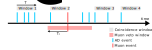
\includegraphics{ch_event_selection/timeline_examples}
    \caption{
        An example timeline showing how coincidence groups are created,
        and how they interact with muons and muon veto windows.
        This illustration does not show the \SI{1}{\micro\second} gap
        at the start of each coincidence window.
        Windows 1, 3, and 4 are valid coincidence groups,
        while Window 2 is vetoed by the muon event.
    }
    \label{fig:timeline_examples}
\end{figure}

Because of the initial \SI{1}{\micro\second} gap,
the actual time interval covered by any given coincidence window is
$\tc - \SI{1}{\micro\second}$.
This analysis uses a coincidence search window of $\tc = \SI{1.5}{\milli\second}$.

The total number of AD events in the group
is the multiplicity of the group.
A coincidence group with multiplicity $n$ is also referred to
as an \fold{n} coincidence.
In Window 1 of \cref{fig:timeline_examples},
the first AD event starts a new coincidence window
that includes three other AD events,
resulting in a coincidence group of multiplicity 4, or a \fold{4} coincidence.

If a muon event occurs within a coincidence window,
then that coincidence window is vetoed.
In other words, every muon has an implicit veto window
that forbids prompt events within \tc{} of the muon.
This is demonstrated by Window 2 of \cref{fig:timeline_examples}.
Note that if the prompt event occurs earlier than \tc{} before a muon,
then subsequent events within the coincidence window
are allowed to occur inside of the implicit muon veto window.
Only prompt events are vetoed by the implicit veto window.

The veto window after a muon also impacts the way that
coincidence windows are formed.
Window 3 of \cref{fig:timeline_examples} shows a coincidence window
whose prompt event is preceded by other recent AD events.
However, those AD events fall within the previous muon veto window,
so they are ignored for the purposes of forming coincidence groups.

If a prompt event has no subsequent AD events within \tc, it is
still a valid group, and is referred to as a \fold{1} coincidence.
Note that \fold{1} coincidences are somewhat but not strictly isolated
from other AD events.
Certainly there are no other AD events
within \tc{} \textit{after} the prompt event,
but there may be a \textit{preceding} AD event within \tc{}
if that event is part of a coincidence window
which ends before the prompt event in question.
Window 4 of \cref{fig:timeline_examples} demonstrates this property:
there are no other AD events within Window 4,
but there is a previous AD event within \tc{} of the start of Window 4.
Given the event rates at Daya Bay, this only happens in $\sim10^{-4}$
of single events.
This probability is derived in \cref{ap:singlesformula} as $P_b$.

\newcommand{\adheight}{0.23\textheight}
\newcommand{\adspacing}{1cm}
\newcommand{\adinclude}[1]{
    \includegraphics[height=\adheight, trim={0 0 0 1cm}, clip]{#1}
}
\newcommand{\adgrid}[3]{
    \begin{figure}
        \centering
        \adinclude{#3_EH1_AD1}
        \hspace{\adspacing}
        \adinclude{#3_EH1_AD2}\\
        \adinclude{#3_EH2_AD1}
        \hspace{\adspacing}
        \adinclude{#3_EH2_AD2}\\
        \adinclude{#3_EH3_AD1}
        \hspace{\adspacing}
        \adinclude{#3_EH3_AD2}\\
        \adinclude{#3_EH3_AD3}
        \hspace{\adspacing}
        \adinclude{#3_EH3_AD4}
        \caption{#1}
        \label{#2}
    \end{figure}
}

\adgrid{All double coincidences found using $\tc=\SI{1.5}{\milli\second}$}{fig:double_coinc_raw}{ch_event_selection/double_coincs}

Once the coincidence groups have been constructed,
the set of \fold{2} coincidences can be identified as
the preliminary set of IBD candidates,
albeit with background still present.
\Cref{fig:double_coinc_raw} shows the prompt and delayed energy
of all \fold{2} coincidences identified in EH1-AD1 and EH3-AD1
as representatives of the near and far sites.
These plots clearly show the nGd events
at delayed energy values near \SI{8}{\mev}.
The nH events are visible as the narrow band at
delayed energies near \SI{2.2}{\mev}
and prompt energies of \SIrange{4}{7}{\mev}.
At prompt energies less than \SI{3.5}{\mev} or greater than \SI{7}{\mev}
these signal events are overwhelmed by the accidental background,
which is characterized in these plots by the 4-point square at both prompt and
delayed energies of \SIlist{1.5;3.25}{\mev}.

The \fold{1} coincidences can be identified as a subset
of the uncorrelated events, mostly radioactive decays,
that are also present in the data stream.
However, not all uncorrelated events end up in \fold{1} coincidences.
Sometimes an uncorrelated event will occur in close proximity to
a true IBD prompt-delayed pair, creating a \fold{3} coincidence.
These high-multiplicity coincidence groups are vetoed
with a small loss of efficiency.
More concerning is when two uncorrelated events
randomly occur in close proximity to each other,
creating a \fold{2} coincidence group that passes the high-multiplicity veto.
These so-called ``accidental'' coincidences
constitute the largest background within the set of \fold{2} coincidences
(\cref{subsec:acc}).
The distance, time and energy cuts described below
are all motivated in large part by the need to reduce the accidental background.

\section{Distance and time cuts}

The distance and time distributions between prompt and delayed AD events
are different depending on the physical process producing those AD event pairs.
For example, the neutron produced during an IBD interaction
scatters within the liquid scintillator until being captured
by a hydrogen nucleus,
traveling a characteristic distance over a characteristic time.
On the other hand, two uncorrelated events have, by definition,
no particular connection between their physical locations
or their timings.

In practice, the characteristic distance for a neutron capture on hydrogen
is approximately \SI{200}{\milli\meter},
and the characteristic time delay is \SI{200}{\micro\second}.
For accidental coincidences, the characteristic distance is
the length scale of the AD, approximately \SI{3000}{\milli\meter},
and the time delay has a flat probability distribution
on the time scale used for the coincidence window ($\tc = \SI{1.5}{\milli\second}$).

\adgrid{Distribution of coincidence distance and coincidence
time}{fig:dr_vs_dt}{ch_event_selection/dr_vs_dt}

\Cref{fig:dr_vs_dt} shows the distribution of
coincidence distance and coincidence time
for the subset of \fold{2} coincidences with
relatively small coincidence distances and times
of less than \SI{1000}{\milli\meter} and \SI{600}{\micro\second},
respectively.
Correlated events are grouped at the lowest
coincidence times and distances,
although there is a visible tail in both dimensions.
The rest of the events distributed with relatively uniform density
across the plot are accidental background from uncorrelated events.
This plot was used to determine the distance and time cut
by drawing a line from \SI{800}{\milli\meter} at $0$ time
to \SI{480}{\micro\second} at $0$ distance.
This line rather effectively separates the higher-density region
of correlated events from the uniform density region of accidental background.
This cut is known as the DT cut and the line determining the cut has the equation

\begin{equation}
    \text{DT} = \Delta r + v_0 \Delta t < \SI{800}{\milli\meter},
\end{equation}
where $v_0 = \frac{\SI{1000}{\milli\meter}}{\SI{600}{\micro\second}}$.
Note that the quantity DT is not D times T,
nor should it be confused the differential $dt$.
\Cref{fig:after_DT_cut} shows the individual AD spectra
after applying the DT cut.
As expected, the accidental background present
in the low-prompt-energy and low-delayed-energy corner is much reduced.
The neutron capture on hydrogen events now stand out much better
against the accidental background.

\adgrid{Prompt-delayed energy spectra after applying
the DT cut}{fig:after_DT_cut}{ch_event_selection/post_DT_cut}

Applying the DT cut rejects the vast majority of accidental events
at a loss of approximately \SI{30}{\percent} of real IBDs.
The efficiency is measured after subtracting the accidental background
(\cref{subsec:acc})
by comparing the number of \fold{2} coincidences that pass the energy cuts and the DT cut
with the number of \fold{2} coincidences that pass the energy cuts
and a significantly relaxed DT cut of \SI{3000}{\milli\meter}:

\begin{equation}
    \varepsilon_{\text{DT}} = \frac{N(\text{DT} < \SI{800}{\milli\meter})}{
    N(\text{DT} < \SI{3000}{\milli\meter})}
\end{equation}
As the histograms in \cref{fig:ed_DT_sub} show,
negligibly few IBDs have a DT value anywhere close to \SI{3000}{\milli\meter},
so $\varepsilon_{\text{DT}}$ closely approximates the true efficiency.
The DT cut efficiency for each AD is shown in \cref{fig:DT_eff}.

\begin{figure}
    \centering
    \includegraphics[width=0.49\textwidth, trim={0 0 0 1cm}, clip]{%
        ch_event_selection/ed_DT_sub_EH1_AD1%
    }
    \includegraphics[width=0.49\textwidth, trim={0 0 0 1cm}, clip]{%
        ch_event_selection/ed_DT_sub_EH2_AD1%
    } \\
    \includegraphics[width=0.49\textwidth, trim={0 0 0 1cm}, clip]{%
        ch_event_selection/ed_DT_sub_EH3_AD1%
    }
    \caption{
        The accidentals-subtracted distribution of
        delayed energy and DT value, used to compute $\varepsilon_{\text{DT}}$.
        The green (solid) box shows the events included in the DT cut.
        The black (dashed) box shows the events excluded by the DT cut.
        The large fluctuations at high DT are due to the statistics
        of subtracting two almost-equal large numbers as part of the
        background subtraction procedure.
    }
    \label{fig:ed_DT_sub}
\end{figure}

\begin{figure}
    \centering
    \includegraphics[height=0.4\textheight]{plot_diagnostics/distance_time_cut_efficiency}
    \caption{The DT cut efficiency for each AD. Error bars are statistical.}
    \label{fig:DT_eff}
\end{figure}

The AD-uncorrelated uncertainty for the efficiency
is determined from the data by examining the variation
in measured efficiency between the 4 near-hall ADs.
The far-hall ADs are excluded because
their statistical uncertainties are much larger than the
near-hall AD variation.
The AD-uncorrelated uncertainty of the DT cut efficiency
is the half-range of the near-hall efficiencies: \num{0.0016} (absolute),
or approximately \SI{0.23}{\percent} (relative).

\section{Energy cuts}

\subsection{Prompt energy}
The prompt energy lower bound of \SI{1.5}{\mev}
is chosen to exclude a substantial fraction
of the low-energy uncorrelated events from radioactive decays.
In particular, the electron capture process
${}^{40}\text{K} \to {}^{40}\text{Ar} + \nu_e + \gamma$
releases a $\gamma$ ray with energy \SI{1.46}{\mev}.
The high-energy tail of this interaction is visible in the prompt-delayed spectra
(\cref{fig:double_coinc_raw}) as an elevated bin content
along both the horizontal and vertical axes from \SIrange{1.5}{3}{\mev}.

\begin{figure}
    \centering
    \includegraphics[width=0.6\textwidth, trim={0, 1.5cm, 0, 0}, clip]{%
        ch_event_selection/prompt_energy_mc%
    }
    \caption{The spectrum of reconstructed energy for IBD prompt events
        in the Monte Carlo study used to compute the prompt energy efficiency
    and AD-uncorrelated uncertainty}
    \label{fig:prompt_eff_mc}
\end{figure}
The nominal efficiency of the prompt energy cut is estimated using Monte Carlo.
The spectrum of ``true'' IBD prompt event reconstructed energy
is shown in \cref{fig:prompt_eff_mc}.
Only events with energy above \SI{1.5}{\mev} on this histogram
are included in the IBD event selection.

%TODO figure
However, because of the energy dependence of the \nuebar{} oscillations,
a different fraction of \nuebar{} will pass this cut
depending on the baseline between the reactor and the AD.
For example, at shorter baselines, low-energy \nuebar{}
are more likely to oscillate to other flavors, so that at the near halls,
there are fewer IBD events missed by the prompt energy cut,
thus raising the efficiency of the cut.
At the oscillation maximum, though, medium-energy \nuebar{},
around \SIrange{2}{3}{\mev}, are most likely to oscillate.
So a smaller fraction of IBDs will pass the cut,
and the efficiency will be lower.

Corrections for each AD--reactor pair should be computed
and weighted to arrive at each AD's final prompt energy efficiency.
Since the corrections to the efficiency depend on
the amplitude of \nuebar{} oscillations, they rely on knowledge of \thetaot.
(For example, there would be no corrections at all if \thetaot{} were $0$.)
To compute accurate corrections and, more importantly, an accurate value
for \thetaot{}, an iterative process is used.
Initially, no baseline-dependent correction is used and
a value for \thetaot{} is obtained.
That initial \thetaot{} is then used to compute baseline-dependent corrections,
and the updated efficiencies are used to compute an updated value for \thetaot{}.
This process is repeated until the \thetaot{} result converges.
%TODO figure

The AD-uncorrelated uncertainty for the prompt energy lower bound
is dominated by differences in the energy scale between ADs.
Based on the analysis of the delayed energy spectrum in each AD
reported in \cref{subsec:delayed}, the energy scale
varies by less than \SI{0.5}{\percent} between ADs.
By applying a \SI{+-0.5}{\percent} variation to
the event energy in the Monte Carlo dataset as visualized in \cref{fig:prompt_eff_mc},
the impact of the energy scale differences can be propagated
to the prompt energy efficiency.
The impact, and therefore the relative uncertainty on
the prompt energy efficiency, is observed to be \SI{0.1}{\percent}.

There is also a \SI{12}{\mega\electronvolt} upper bound for the prompt energy.
The reactor \nuebar{} spectrum falls steeply above \SI{8}{\mev},
so this cut is determined to have \SI{100}{\percent} efficiency.

\subsection{Delayed energy}
\label{subsec:delayed}

Neutron capture on hydrogen releases a (monoenergetic)
\SI{2.22}{\mev} $\gamma$-ray,
which means the cut values can be tuned to a narrow energy region
around that value.
However, while the prompt IBD positron essentially never escapes
from the liquid scintillator sensitive volume,
$\gamma$'s do regularly escape (a few percent of the time),
depositing less than their full energy in the liquid scintillator.
Both the tuning of the energy cut values
and the fraction of escaping $\gamma$'s are sensitive to
small variations in the geometry of the AD, energy reconstruction,
and scattering properties of $\gamma$'s in
both liquid scintillator and in acrylic.

The delayed energy cut bounds are identified based on
functional fits to each AD's delayed energy spectrum.
Specifically, the spectrum is generated by first applying
the prompt energy cut and DT cut,
then statistically subtracting the accidental background (\cref{subsec:acc}).
Although the resulting spectrum still has some background,
the only remaining background processes also involve
neutron capture on hydrogen, and contribute to the same spectral shape
as the signal IBD process.

Each spectrum is fit with the calorimeter function, which models
a calorimetric response to a monoenergetic process with ``true''
energy $\mu$.
The modeled detector has an intrinsic and energy resolution $\sigma$
which applies a Gaussian smearing to the deposited energy.
($\sigma$ itself is independent of energy.)
While many events in this model deposit all of their energy into
the calorimeter, some events partially leak out.
The fraction of events that deposit their full energy in the detector
is referred to as the peak fraction $\alpha$.
The energy leakage is modeled as an exponential distribution
with characteristic energy scale (or ``tail slope'') $\lambda$.
The fit function itself is derived by starting with
the unsmeared model:

\begin{equation*}
    f_{unsmeared}(E) =
    \begin{cases}
        \alpha\delta(E-\mu) + (1-\alpha)\lambda e^{\lambda E}
        & 0 < E \leq \mu \\
        0 & E > \mu
    \end{cases}
\end{equation*}
This function is then convolved with a Gaussian
of width $\sigma$.

\begin{align*}
    f_{cal}    &= f_{unsmeared} \otimes \text{Gaussian} \\
    f_{cal}(E) &= \int_0^\mu dE' f_{unsmeared}(E') \cdot \text{Gaussian}(E'-E; \mu) \\
               &= \frac{1}{\sigma\sqrt{2\pi}}
               \left[
                   \alpha\int_0^\mu dE' e^{-\frac{(E'-E)^2}{2\sigma^2}} \delta(E'-\mu)
                   + (1-\alpha)\int_0^\mu dE' e^{-\frac{(E'-E)^2}{2\sigma^2}}
                   \lambda e^{\lambda E'}
               \right] \\
               &= \alpha\frac{1}{\sigma\sqrt{2\pi}}e^{-\frac{(E-\mu)^2}{2\sigma^2}}
               + (1-\alpha)
               \frac{\lambda e^{\sigma^2\lambda^2+2\lambda E}}{e^{\lambda\mu}-1}
               \left[
                   \text{erf}
                   \left(
                       \frac{\mu-E-\sigma^2\lambda}{\sigma\sqrt{2}}
                   \right)
                   + \text{erf}
                   \left(
                       \frac{E + \sigma^2\lambda}{\sigma\sqrt{2}}
                   \right)
               \right]
\end{align*}
The entire result is normalized to unity
but can be scaled by an overall normalization $N$.

\adgrid{Delayed energy fits using the calorimeter function}{fig:delayed_fits}{%
    ch_event_selection/delayed_fit%
}

\begin{figure}
    \centering
    \includegraphics[height=0.33\textheight]{plot_diagnostics/delayed_energy_peak.pdf}
    \vspace{0.5cm}\hspace{0.5cm}
    \includegraphics[height=0.33\textheight]{plot_diagnostics/delayed_energy_width.pdf}\\
    \includegraphics[height=0.33\textheight]{plot_diagnostics/delayed_energy_expo_scale.pdf}
    \hspace{0.5cm}
    \includegraphics[height=0.33\textheight]{plot_diagnostics/delayed_energy_peak_frac.pdf}\\
    \caption{
        Fit parameters for each AD.
        Error bars represent fit errors.
        The smaller plots show the relative deviation of each AD's value
        from the average value of the 4 near-hall ADs.
    }

    \label{fig:delayed_fit_parameters}
\end{figure}

\begin{table}[ht]
    \centering
    \begin{tabular}[t]{lllll}
        \hline
        & Peak energy [\si{\mev}]
        & Width [\si{\mev}]
        & Tail slope [\si{\per\mev}]
        & Peak fraction \\
        \hline
        EH1-AD1 & \num{2.2531} & \num{0.1365} & \num{1.6893} & \num{0.8683}\\
        EH1-AD2 & \num{2.2551} & \num{0.1380} & \num{1.6247} & \num{0.8666}\\
        EH2-AD1 & \num{2.2591} & \num{0.1351} & \num{1.7212} & \num{0.8663}\\
        EH2-AD2 & \num{2.2602} & \num{0.1348} & \num{1.7319} & \num{0.8902}\\
        \hline
        EH3-AD1 & \num{2.2607} & \num{0.1360} & \num{1.5812} & \num{0.8667}\\
        EH3-AD2 & \num{2.2622} & \num{0.1349} & \num{2.1516} & \num{0.8616}\\
        EH3-AD3 & \num{2.2563} & \num{0.1366} & \num{1.3432} & \num{0.8507}\\
        EH3-AD4 & \num{2.2682} & \num{0.1362} & \num{2.5653} & \num{0.8617}\\
        \hline
    \end{tabular}
    \caption{Delayed energy fit parameters}
    \label{tab:delayed_fit_params}
\end{table}

\begin{table}[ht]
    \centering
    \begin{tabular}[t]{lll}
        \hline
        & Lower bound [\si{\mev}]
        & Upper bound [\si{\mev}] \\
        \hline
        EH1-AD1 & \num{1.8435} & \num{2.6628}\\
        EH1-AD2 & \num{1.8412} & \num{2.6690}\\
        EH2-AD1 & \num{1.8537} & \num{2.6645}\\
        EH2-AD2 & \num{1.8558} & \num{2.6646}\\
        \hline
        EH3-AD1 & \num{1.8527} & \num{2.6686}\\
        EH3-AD2 & \num{1.8575} & \num{2.6669}\\
        EH3-AD3 & \num{1.8467} & \num{2.6660}\\
        EH3-AD4 & \num{1.8597} & \num{2.6768}\\
        \hline
    \end{tabular}
    \caption{Delayed energy cut bounds derived as $\mu \pm 3\sigma$}
    \label{tab:delayed_bounds}
\end{table}

\begin{figure}
    \centering
    \includegraphics[height=0.40\textheight]{plot_diagnostics/delayed_energy_bounds.pdf}
    \caption{
        Delayed energy cut bounds computed as $\mu\pm 3\sigma$
        from the fitted histograms
    }
    \label{fig:delayed_bounds}
\end{figure}

The eight delayed energy spectra with their fits are shown in \cref{fig:delayed_fits}.
Comparing the fitted parameters across ADs can be used
to measure the identicalness of the ADs.
Their values and relative differences are plotted in \cref{fig:delayed_fit_parameters}
and listed in \cref{tab:delayed_fit_params}.
In particular, the top-left plot shows the relative difference
in the fitted peak $\mu$ across the ADs,
which is a measure of the energy scale variation.
The relative variation of \SI{+-0.5}{\percent}
is used to compute the AD-uncorrelated uncertainty
on the prompt energy cut efficiency.

The bounds for the delayed energy cut are computed
based on the fitted peak value and energy resolution
from the calorimter model. The energy criterion is

\begin{equation}
    \mu - 3\sigma < E < \mu + 3\sigma.
\end{equation}
This form was decided on even though the calorimeter function
is not symmetric, and even though in reality
the detector resolution changes with energy
(and therefore is not precisely modeled in the fit).
The values used for the energy bounds are listed in \cref{tab:delayed_bounds}
and plotted in \cref{fig:delayed_bounds}.

The absolute efficiency of the delayed energy cut
is measured using Monte Carlo.
The same fitting procedure with the calorimeter function
and the same $\mu \pm 3\sigma$ bounds are used to
estimate the fraction of neutron capture on hydrogen events
that pass the delayed energy cut.
The relative fraction of GdLS to LS also impacts the efficiency
because with more GdLS, fewer neutrons will capture on hydrogen.
This difference between the GdLS and LS regions is taken into account
when computing the absolute efficiency.
The estimated absolute efficiency for the delayed energy cut
is \SI{40}{\percent}.
About half of the inefficiency is due to captures on Gd in the GdLS region,
and the other half is due to escaping neutrons or escaping $\gamma$-rays
from the LS (outer) region of the AD.

\begin{figure}
    \centering
    \includegraphics[height=0.4\textheight]{ch_event_selection/delayed_eff_uncertainty_cartoon}
    \caption{
        Intuition for how differences in the relative size
        of the nominal (peak) versus extended ranges
        are a proxy for differences in cut efficiency.
    }
    \label{fig:delayed_eff_unc_cartoon}
\end{figure}

The AD-uncorrelated uncertainty on the efficiency
includes variations due to all the above effects:
geometrical variations, energy scale, different material properties,
Gd fraction, etc.
The overall variation between ADs is estimated using a general method
that compares the relative size between the peak and tail regions
of the delayed energy spectrum, as defined by the delayed energy cut,
across the ADs.
Intuitively, if the same fraction of events is in the peak region in each AD,
then the cut efficiency must have a small variation.
This intuition is visualized in the cartoon in \cref{fig:delayed_eff_unc_cartoon}.
The ``expected'' curve has a high efficiency
and few events in the tail.
Since the ``different tail'' curve has more events in the tail region,
it can be concluded that this curve has a lower efficiency.

In practice, it is easier to compare the number of events in the peak
to the total number of events in an extended region that includes the tail,
rather than to just the new events in the tail.

For each AD's delayed energy spectrum, the peak region is defined as
the region passing the delayed energy cut, $\vert E-\mu \vert < 3\sigma$.
The extended region is the same for each AD:
$\SI{1.5}{\mev} < E < \SI{2.8}{\mev}$.
Using an AD-dependent definition for the peak region but
the same values for the extended creates
the desired sensitivity to variations in the energy scale.
Extending the lower bound down to \SI{1.5}{\mev} adds sensitivity to
anything that would change the shape of the tail
or the fraction of $\gamma$'s that (partially) escape from the AD.

\begin{figure}
    \centering
    \includegraphics[height=0.4\textheight]{ch_event_selection/delayed_uncertainty_fit}\\
    \includegraphics[height=0.4\textheight]{plot_diagnostics/delayed_energy_uncertainty_method1}
    \caption{
        (Top) Data points and (affine) linear fit
        to the number of events in the nominal (peak)
        and extended ranges of delayed energy.
        Statistical error bars are too small to be visible on this plot. \\
        (Bottom) Relative deviations from each hall to the fit model.
        The half-range of deviations for near-hall ADs
        is the delayed energy efficiency AD-uncorrelated uncertainty.
    }
    \label{fig:delayed_eff_unc_fit}
\end{figure}


If the delayed energy spectra have the same shape,
and if the calorimeter function is an appropriate fitting function
for determining the energy cut bounds,
then for some constant $b$ common to all ADs,
$N_{peak,\,i} = b N_{extended,\,i}$ for each AD $i$.
To test this model, an affine linear function is fit
to the values for each AD:

\begin{equation}
    N_{peak,\,pred,\,i} = a + b N_{extended,\,i},
\end{equation}
where $N_{peak,\,pred,\,i}$ is the fit function's prediction
of the actual event count in the peak ($N_{peak,\,i}$).
Plots of $N_{peak,\,i}$ vs. $N_{extended,\,i}$ and of the
relative deviation from the fitted line are shown in \cref{fig:delayed_eff_unc_fit}.
The fit value of $a$ should be $0$ if the simple model of
a linear scaling is correct.
Indeed, the fit value is $a = -321 \pm 387$
which is consistent with $0$.
The fit value for $b$ is $b = 0.9527 \pm 0.0015$,
which can be interpreted as a loose upper bound
on the delayed energy cut efficiency.
The final value for the AD-uncorrelated uncertainty
of the delayed energy efficiency is taken to be
the half-range of the relative deviations
of the near-hall ADs from the fitted line: \SI{0.11}{\percent}.
The far-hall ADs have much higher statistical uncertainty
(relative uncertainty $\approx\SI{0.5}{\percent}$),
and therefore larger fluctuations.
Validation that the far-hall ADs are not
substantially different from the near-hall ADs is obtained by
summing the counts for all 4 far-hall ADs to get
a combined relative deviation for the far hall of \SI{0.018}{\percent},
well within the uncertainty derived from the near halls.




\chapter{Simulation}
\label{ch:simulation}

Monte Carlo simulation (MC) refers to the practice
of estimating the probability distribution of the outcomes
of a complex and non-deterministic chain of events
by running a (pseudo-random) simulation of the process multiple times
and recording the distribution of the simulated outcomes.
MC is commonly used to estimate detection efficiencies,
a detector's energy response,
and other quantities that have a highly nontrivial dependence
on basic geometric and kinematic quantities.

A distinction is often made between a ``full Monte Carlo''
and a ``toy Monte Carlo.''
In a full MC, each particle is propagated through a series of small time steps,
with various probabilities to interact, decay, deposit energy, and/or be detected,
depending on the material being traversed.
As the name suggests, toy MCs adopt simplifications from the full approach,
and these simplifications can vary widely.
One prototypical example is to use the average $dE/dx$
and a particle's propagation distance
(perhaps determined by drawing from an exponential distribution
based on the decay time and velocity)
to determine the amount of energy deposited by a particle
before it decays.
The simplifications made to toy MCs usually limit their validity
to highly specific scenarios.

Three separate toy MC simulations were used in this analysis
to simulate individual IBD events (\cref{sec:thu_toymc}),
Daya Bay reconstructed-data files (\cref{sec:toymc}),
and entire experiments' worth of data (\cref{sec:lbnl_toymc}).

\section{Individual IBD event simulation}
\label{sec:thu_toymc}

The Individual Event Simulation (IES) was designed
to study detection efficiencies and the detector energy response \cite{nh2016technote}.
This simulation was composed of a full, particle-level Monte Carlo simulation
and a toy detector response model.
Each event began as a \nuebar{} of a given energy interacting via IBD
with an atom in a given region of the Daya Bay AD
(GdLS, LS or acrylic).
The interaction products ($e^+$ and $n$),
were simulated using a full MC implemented using the GEANT4 library \cite{geant4}.
The full simulation included
the positron's energy depositions into the scintillator
and its annihilation,
the neutron's thermalization, scattering, and capture on a nucleus (or escape),
and the resulting $\gamma$-rays' propagation and interactions.
The resulting electrons and positrons from the $\gamma$-ray interactions
were also simulated.
During propagation, an electron could
``deposit'' energy in the liquid scintillator,
escape from the scintillating volume,
or scatter and create another energetic electron.
The total amount of deposited energy was saved as $E_{\text{dep}}$.

To obtain a final simulated reconstructed energy,
a parametrized nonlinearity model and resolution were used
rather than implementing the effects in a full MC.
The scintillator and electronics nonlinearities were applied
to the deposited energy $E_{\text{dep}}$
(see \cref{subsec:abs_energyscale}).
The energy resolution (\cref{subsec:resolution}) used in the MC
was modified to reflect
the absence of detector non-uniformity in the simulation
by setting the $a$ parameter to 0 (cf.\ \cref{eq:energy_resolution}):
\begin{equation}
    \frac{\sigma_E}{E} = \sqrt{0 + \frac{b^2}{E} + \frac{c^2}{E^2}}.
\end{equation}

The IES was used to generate a data set
where the incident \nuebar{} spectrum
matched the predicted unoscillated reactor \nuebar{} spectrum.
The distributions of simulated prompt and delayed reconstructed energies,
shown in \cref{fig:prompt_eff_mc},
could be used as estimates of the actual distributions.
In other analyses (e.g.\ \cite{nh2016}), the MC estimates
for absolute efficiencies of the prompt and delayed energy cuts
were computed from this simulation.
In this analysis, the absolute efficiencies were not used.
However, the IES was used to estimate other quantities.

\begin{figure}
    \centering
    \includegraphics[width=0.49\textwidth]{%
        ch_event_selection/prompt_energy_mc%
    }
    \includegraphics[width=0.49\textwidth]{%
        ch_event_selection/delayed_energy_mc%
    }
    \caption[Simulated prompt and delayed spectra]{Spectrum of reconstructed energy for simulated IBD prompt (left)
        and delayed (right) events
        in the Monte Carlo study used to compute the absolute efficiencies
        of the prompt- and delayed- energy cuts.
        The prompt spectrum is also used to compute the
        AD-uncorrelated uncertainty of the prompt-energy cut.
    }
    \label{fig:prompt_eff_mc}
\end{figure}

\subsubsection{Study of prompt energy cut efficiency}

The prompt-energy cut efficiency for each AD depended on
the oscillation parameters due to the energy dependence of \nuebar{} oscillation
(see \cref{subsec:prompt_energy}).
This correction was computed at a given point in parameter space
(value of \thetaot{}, $\Delta m^2_{32}$, and AD-reactor pair)
by creating a histogram of reconstructed prompt energy
where each entry was weighted by the oscillation probabilty
at the ``true'' \nuebar{} energy saved by the simulation.
The resulting efficiency was compared
with the nominal efficiency assuming no oscillation.
The relative difference was applied as a correction
during the near-far projection procedure in \cref{subsec:flux_fraction}.

\subsubsection{Study of relative energy scale}

The prompt-energy spectrum and cut efficiency
both depended on the relative energy scale between ADs
(see \cref{subsec:rel_energyscale}).
A shift in the energy scale was modeled by
creating a histogram of reconstructed prompt energy,
but where the value of the energy was scaled
by the uncertainty of the relative energy scale, \SI{\pm0.5}{\percent}.
The resulting change to the prompt-energy cut efficiency, \SI{\pm0.1}{\percent},
was the AD-uncorrelated uncertainty for that efficiency.
Shifting the energy scale also changed the shape of the spectrum,
which was quantified by comparing the change in number of events
in each bin of the histogram with and without the re-scaled energy values.
The oscillation dependence of the spectral shape was also accounted for.

For a particular bin $b$ of reconstructed energy in AD $i$,
the relative energy scale correction $a_{\text{relE},i}^{(b)}$
was defined as the difference in bin content with and without
the relative energy scale shift of \SI{\pm0.5}{\percent},
divided by the bin content without the shift:
\begin{equation}
    a_{\text{relE},i}^{\pm,(b)}(\thetaot, \Delta m^2_{32}) =
    \frac{N^\pm(\thetaot, \Delta m^2_{32}) - N^0(\thetaot, \Delta m^2_{32})}%
    {N^0(\thetaot, \Delta m^2_{32})},
\end{equation}
where the $+$ refers to scaling the energy by \SI[retain-explicit-plus]{+0.5}{\percent}
and the $-$ refers to scaling by \SI{-0.5}{\percent}.
During the fit procedure to extract \thetaot{} in \cref{ch:analysis}, the impact of this correction
was controlled by a nuisance parameter.
The fitter automatically switched between the $+$ and $-$ values
depending on the sign of the nuisance parameter.

This correction was intentionally not normalized;
the consistent application of $a_{\text{relE},i}^{\pm,(b)}$ to all bins
could change the total number of events.
The impact of the change in total number of events
was equivalent to the previously-mentioned change
to the prompt-energy cut efficiency induced by the relative energy scale shift.
To avoid double-counting the change in number of events
due to a shift in relative energy scale,
the prompt-energy cut efficiency was omitted
from the fit model and from the constraint
on the nuisance parameter representing the overall detection efficiency uncertainty.

\section{Data file simulation}
\label{sec:toymc}

The Daya Bay event selection process (\cref{ch:event_selection})
depended on more than just the properties of each AD event in isolation;
there were anti-coincidence requirements such as the muon veto,
and of course double-coincidence requirements to select IBDs.
Additionally, the basis for the determination of the accidental background rate
relied heavily on the accurate extraction of
the rate of uncorrelated ``single'' events.
Both the event selection and the accidentals characterization
relied on a simple model of the data stream,
with only three distinct event types:
muon events, uncorrelated single events,
and correlated pairs comprising IBD events.
The Reconstructed-Data File Simulation (RDFS)
produced simulated data files in the same format
as the output of the calibration and reconstruction procedure
(``production,'' described in \cref{sec:daq}).
This simulation was used
to study the impact of the assumptions in the data stream model
and to validate the implementation of
the event selection and accidentals characterization
in software.

The RDFS received as input
a specification for the rates of various event types,
representing IBDs, uncorrelated events, muons, etc.,
and a total ``runtime'' representing the amount of AD livetime to simulate.
The configuration could be varied to, for example,
increase the rate of single events
or decrease the capture time delay between prompt and delayed IBD signals.
and the effect of that change could be studied.
To produce a data stream,
first, timestamps were generated for each event
based on the rates for each event type and the total livetime.
Simulated energy and position values were then generated for each event.
Vast simplifications were employed to allow for
extremely fast event generation,
and no attempt was made at creating
physically-realistic distributions for
reconstructed energy or position.
Instead, these distributions were chosen to make analysis
of the selection cuts more convenient.
This was an acceptable compromise since the purpose of the simulation
was to validate properties of the data model,
rather than the traditional goal of estimating specific quantities
which are difficult or impossible to measure using real data.

Simulated events were saved to disk in the same ROOT file data format
used by the Daya Bay data production.
An additional ROOT TTree structure containing the ``truth information''
for each event was included in the output data file.
For this simulation, the truth information for an event consisted simply of
the event type.
A flowchart describing the steps in the simulation
is provided in \cref{fig:my_toymc_flowchart}.
The characteristics associated with the different event types
are described below.

\begin{figure}
    \centering
    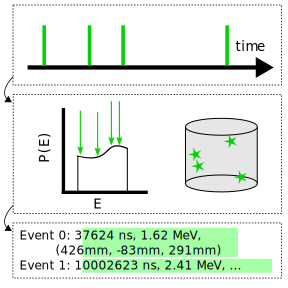
\includegraphics[width=0.49\textwidth]{ch_simulation/singles_flow}
    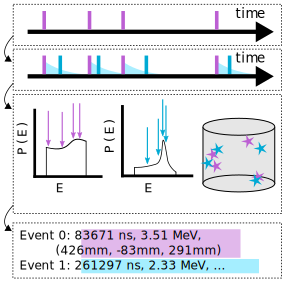
\includegraphics[width=0.49\textwidth]{ch_simulation/correlated_flow}
    \caption[Data stream simulation diagram]{
        The data stream simulation steps
        for Single events (left) and Correlated events (right).
        The steps are event count and timestamps (top),
        energy and position (middle), and serialization (bottom).
        Different colors represent different event types:
        green, violet and blue represent Single,
        prompt Correlated and delayed Correlated,
        respectively.
        The highlight colors in the serialization phase
        represent the ``truth'' information stored separately.
    }
    \label{fig:my_toymc_flowchart}
\end{figure}


The RDFS was based on a core set of event types:
Single, Correlated, and Muon.
Additional event types such as Flasher were added to support specific studies
(see \cref{subsec:toymc_flashers}).
The simulation's configuration allowed for customization of the event rate
for each different event type,
and also for multiple variants of the event type.
For example, one type of Correlated event could be configured to represent nH IBDs,
and a second type could be configured to represent nGd IBDs
with a shorter coincidence time, higher delayed energy,
and with the delayed event's position limited to the GdLS (IAV) region of the AD.

\subsection{Types of generated events}

\subsubsection{Single events}

Single events represented uncorrelated signals,
which in Daya Bay were primarily caused by natural radioactive decays in the AD
(\cref{subsec:singles}).
In the simulation, Single events were assigned timestamps
drawn uniformly at random between the runtime limits given in the configuration,
representing their uncorrelated nature.
The event energies were also drawn uniformly at random
between \SIlist{1;3.5}{\MeV},
and the positions were randomly assigned
within the scintillating volume.
(The energy and position distributions can both be customized through plug-ins
but were left at their defaults for the studies described here.)

\subsubsection{Correlated events}

Correlated events represented pairs of signals
with a common physical origin, both in position and in time.
IBDs and correlated backgrounds (\cref{sec:correlated_bg})
satisfied these criteria and could be modeled by the Correlated event type.
To create the time correlation between prompt and delayed events,
modeled as an exponential distribution,
the simulation first determined the timestamp for a prompt event at random.
Then the coincidence time delay between prompt and delayed events was generated
from an exponential distribution
whose time constant was specified in the simulation configuration.
The prompt and delayed energies were determined independently at random
using distributions specified by the simulation configuration.
The position of the prompt event was chosen at random
within the GdLS or LS volumes (again, as specified by the configuration),
and the delayed position was chosen to be correlated with the prompt position.
Since exact modeling of the position correlations was not crucial for the studies
performed with the RDFS,
a simple exponential distribution was used to determine the displacement
in each direction ($x,y,$ and $z$) for these Correlated events.
In the recorded truth information,
prompt and delayed events are assigned separate labels.

\subsubsection{Muon events}

Muon events represented signals created by muons traversing
the water pools and ADs (\cref{sec:muonveto}).
For simplicity, each muon was assumed to create a signal
in the inner water pool with a probability of \SI{100}{\percent}.
The rates and energies were chosen to approximately model
the true distributions and rates of muon signals in the near halls (EH1 and EH2).
A portion of the muon signals, \SI{19.95}{\percent},
were assumed to traverse the AD, depositing an energy chosen at random between
\SIlist{20;2000}{\MeV}.
A smaller subset of the muon signals, \SI{0.05}{\percent},
were simulated as showering muons and deposited an energy chosen at random between
\SIlist{2500;5000}{\MeV}.
The time delay between WP and AD muons was assigned to be \SI{50}{\ns},
chosen since in real data there was a nonzero time offset between WP and AD muons;
however, the precise distribution of time offsets between WP and AD muon readout signals
was not a critical feature of the event selection.
All of the choices of energies and rates were approximations
designed to capture the general behavior of muons at Daya Bay
without adding excessive complexity to the simulation.

\subsection{Study of uncorrelated-event rate}
\label{subsec:sim_singles}

The procedure for determining the uncorrelated-event rate
is described in \cref{subsec:singles}.
This process, both the abstract algorithm and the actual software implementation,
was validated using simulated datasets.
The RDFS was configured to generate Single (uncorrelated) events
with a rate of \SI{20}{\Hz}
in data files also containing Muon and Correlated events
representing both nH and nGd IBDs.
The full configuration is listed in \cref{tab:toymc_singles_config}.
100 simulated data files were generated,
each containing 1000 minutes' worth of data.
The data files were processed using the event selection software
and an empirical rate for uncorrelated events was extracted
for each of the 100 files.
The distribution of measured uncorrelated event rates
is shown in \cref{fig:toymc_singles_dist}.
The mean rate over all 100 data sets
was \SI{19.9966+-0.0022}{\Hz},
which is a bias of \SI{0.017}{\percent} or 2 standard deviations.
This bias was considered acceptable
since the accidentals rate uncertainty
for the actual data set was approximately \SI{0.077}{\percent}.
Thus the simulation was able to confirm that
the event selection software could successfully extract
the uncorrelated-event rate with high precision and tolerable bias.

\begin{table}[ht]
    \centering
    \begin{tabular}[t]{lSlS}
        \toprule
        Event type & {Rate [\si{\Hz}]} & Energy [\si{\MeV}] & {Coincidence time [\si{\us}]}\\
        \midrule
        Single & 20. & $[\num{1.5}, \num{3}]$ & {-}\\
        Correlated prompt (nH) & 0.005 & [0.7, 4] & {-} \\
        Correlated delayed (nH) & {-} & [1.9, 2.3] & 150. \\
        Correlated prompt (nGd) & 0.0067 & [0.7, 4] & {-} \\
        Correlated delayed (nGd) & {-} & [7, 9] & 28. \\
        Water Pool Muon & 200. & - & {-} \\
        AD Muon & 39.9 & [\num{20}, \num{2000}] & {-}\\
        Showering Muon & 0.1 & [\num{2500}, \num{5000}] & {-}\\
        \bottomrule
    \end{tabular}
    \caption[Uncorrelated event simulation inputs]{
        Simulation configuration inputs for the uncorrelated-event rate study.
        The rates, energies and coincidence times were simplified
        to allow for faster simulation,
        and no results based on the specific distributions of these quantities
        were used in the final analysis.
    }
    \label{tab:toymc_singles_config}
\end{table}

\begin{figure}
    \centering
    \includegraphics[width=0.7\textwidth]{ch_simulation/singles_rate_unbiased_dist}
    \caption[Extracted simulated uncorrelated event rates]{
        Distribution of uncorrelated event rates over 100 simulated data sets.
        The simulation configuration (``truth'') specified a rate of \SI{20}{\Hz}.
        Each data set consists of a single 1000-minute data file.
    }
    \label{fig:toymc_singles_dist}
\end{figure}

\subsection{Study of residual flashers}
\label{subsec:toymc_flashers}

Light emission by PMTs caused a background of single events
known as flashers \cref{sec:flashers}.
The vast majority of flasher events were rejected using an event-by-event veto,
and the remaining flashers were assumed to be accounted for
by the treatment of the accidental background (\cref{sec:acc}).
Certain PMTs were observed to flash with a frequency
of approximately \SI{0.1}{\Hz},
but with the restriction that
the same PMT never flashed twice within $\lesssim$\SI{0.7}{\s}
(see \cref{fig:flasher_anticorr}).
This pattern violated the assumption in the accidental background analysis
that all single events were uncorrelated and governed by Poisson statistics.
A Flasher event type was added to the RDFS to test the impact of this deviation.

The Flasher event type had a fixed energy and position.
Generated Flasher events were assigned fixed, deterministic timestamps \SI{1}{\s} apart
to simulate a maximally-anticorrelated process with no possible time coincidences.
A data sample was generated with only Single events and Flasher events,
and was treated as if the Flasher events passed the flasher veto criteria.
The Single events had the same configuration as in \cref{tab:toymc_singles_config},
and the Flasher events were assigned a fixed energy of \SI{2.7}{\MeV}.
The accidental background analysis was performed on this data sample (\cref{sec:acc});
after subtracting the accidental background,
the expectation was that 0 correlated events should remain.
\Cref{fig:sim_flasher_prompt_delayed} shows the result of the prompt-delayed spectrum
after subtracting the accidental background
for simulated samples with and without Flasher events \cite{flasher_sim}.
The sample including the Flashers shows
an inaccurate background-subtracted spectrum
due to the synthetic background sample containing unphysical Flasher-Flasher pairs.
In the ``real'' (simulated) data set,
there were no accidental coincidences between Flasher events by construction,
since they were generated with \SI{1}{\s} time gaps
between consecutive Flashers.
This simulation was intentionally configured to exaggerate the impact
of the properties of residual flashers.
This result informed the decision to find ways to veto the residual flasher events
rather than attempt to correct for them in other ways.

\begin{figure}
    \centering
    \includegraphics[width=0.73\textwidth]{ch_simulation/flasher_prompt_delayed}
    \caption[Simulated residual flashers impact]{
        Accidentals-subtracted prompt vs. delayed energy for simulated data samples
        including only Single events (top) or Single and Flasher events (bottom).
        The Singles-only histogram correctly shows 0 events remaining
        after subtracting the accidental background.
        In the with-Flashers histogram,
        the single energy bin containing (\SI{2.7}{\MeV}, \SI{2.7}{\MeV})
        (the energy of the simulated Flasher events)
        has a negative bin content,
        validating that the Flasher events
        will contaminate the synthetic accidental background,
        form Flasher-Flasher pairs, and cause a distortion to the subtracted spectrum.
        Figure taken from \cite{flasher_sim}.
    }
    \label{fig:sim_flasher_prompt_delayed}
\end{figure}

\section{Fake experiment simulation}
\label{sec:lbnl_toymc}

An independent simulation was implemented
to generate spectra of reconstructed prompt energy for each AD,
under assumptions of a wide variety of systematic uncertainties,
backgrounds, and reactor parameters.
Since the simulation output was designed to include all the necessary inputs
to the \thetaot{} fitter,
the outputs were known as ``fake experiments;''
the simulation itself will be referred to as the Fake Experiment Simulation (FES).
This simulation was originally \cite{lbnl_toymc,p12e_fitter,p14a_fitter} designed to generate covariance matrices for
and validate the performance of
one of the fitter programs for the nGd analysis
(Method A of \cite{ngd2016}).
It was used essentially unmodified to validate the fitter for this (nH) analysis
(\cref{ch:analysis}).

The FES received as input predicted \nuebar{} flux and spectrum data
which were computed \cite{christine_reactor} based on data from the reactor operator
and the models by Huber \cite{reactor_huber}
and Mueller \emph{et al.} \cite{reactor_mueller} (see also \cref{sec:reactor}).
For each reactor-AD pair, the spectra were evolved
based on the configured oscillation parameters
and suppressed by $1/L^2$ due to isotropic emission.
The true \nuebar{} spectrum for IBD interactions was computed
based on the IBD cross section \cite{ibd_xsec,ibd_xsec_note},
number of target protons, and the projected reactor flux.
The detection efficiencies and muon and multiplicity veto efficiencies
were also applied.
A model for the detector response was applied to the true interaction energy
to account for the conversion to positron energy,
energy losses in the IAV,
energy nonlinearities in the scintillator and electronics,
and the energy resolution.
The final simulated energies could be scaled by a fixed factor
to account for the relative energy scale uncertainty.
All of the quantities just mentioned could be configured
to be either known or uncertain, in which case
the relevant values in the simulation would be
adjusted by a configurable random amount
to simulate a systematic uncertainty.
Predicted rates and spectra for background events
were added after the IBD prompt spectra were fully generated.
The backgrounds could be randomly fluctuated to account for
uncertainties in their rates and spectra.
Lastly, the number of events in each bin of prompt reconstructed energy
could optionally be fluctuated to account for statistical uncertainty
before being output as the results of the simulation.
\Cref{fig:lbnl_toymc_flowchart} shows the above steps as a flowchart.

\begin{figure}
    \centering
    \includegraphics[width=0.6\textwidth]{ch_simulation/lbnl_toymc_flowchart}
    \caption[Flowchart of data set toy Monte Carlo]{
        Steps to simulate the prompt reconstructed spectra
        at each AD.
        Figure taken from \cite{lbnl_toymc}.
    }
    \label{fig:lbnl_toymc_flowchart}
\end{figure}

\subsection{Study of fitter accuracy}
\label{subsec:fitter_validation}

The fitter developed in \cref{ch:analysis} was validated
using simulated data sets with known values of \thetaot{}.
The degree to which the fitter could extract
the ``correct'' (input) value of \thetaot{}
was a measure of its accuracy
and helped verify that there were no major software bugs
which could have caused an incorrect measurement of \thetaot{}.
The nH and nGd analyses were similar enough
that the same fitter software could be used for both analyses
simply by adjusting the values for uncertainties, efficiencies,
target masses and backgrounds
(and, of course, using the corresponding prompt-energy spectra).
Thus the data set toy Monte Carlo was used without modification
to generate simulated nGd data sets,
and the fitter was validated without relying on
any aspects of the nH analysis.

Data sets were generated under each test configuration
for 36 pairs of (\thetaot{}, \dmee{}) mixing parameters.
(\dmee{} was used only as an input value,
and was converted to $\Delta m^2_{32}$ internally.)
The input values of $\sin^22\thetaot{}$ ranged from 0.065 to 0.09
in steps of 0.005;
those of \dmee{} ranged from
\SI{2.3e-3}{\eV\squared} to \SI{2.7e-3}{\eV\squared}
in steps of \SI{0.08e-3}{\eV\squared}.

The fitter was tested against data sets
that were configured to have no statistical or systematic fluctuations
in order to verify the precise performance
of the prediction algorithm and minimizer.
Since these simulations were fully deterministic,
only one data set was generated for each of the 36 parameter combinations.
The fitter was also tested against data sets
that included fluctuations, both statistical and systematic in nature.
To thoroughly exercise the fitter's functionality
for each configuration,
1000 data sets were generated
for each of the 36 parameter combinations,
for a total of \num{36000} simulated data sets per configuration.
The full listing of configurations tested
is shown in \cref{tab:validation_configs}.
For the final validation, with all systematic and statistical fluctuations
and all pull parameters enabled,
a smaller sample of 190 data sets for each of 9 parameter combinations
(total of \num{1710} data sets)
was used since the full fitter with all pull parameters
took substantially longer to run than it did with any subset of pull parameters.

\ctable[
cap = Fitter validation simulation configurations,
caption = {
    Simulation configurations for validating the fitter performance.
},
label = tab:validation_configs,
pos = ht
]{ll}{
    \tnote[a]{
        Composite nonlinearity functions were generated
        from 5 independent models
        each contributing in random proportions to the composite.
    }
    \tnote[b]{
        Uncertainties from non-equilibrium isotopes,
        spent nuclear fuel contribution,
        correlated and uncorrelated model uncertainties.
    }
}{\FL
    & Fluctuation RMS \ML
    Statistics (EH3) & Poisson \NN
    Statistics (EH1 \& EH2) & Poisson \NN
    Detection efficiency & \SI{0.3}{\percent} \NN
    Relative energy scale & \SI{0.2}{\percent} \NN
    Absolute energy scale & $\lesssim\SI{2}{\percent}$\tmark[a] \NN
    Energy resolution & $\SI{0.2}{\percent}/\sqrt{E/\si{\MeV}}$ \NN
    Reactor power & \SI{0.8}{\percent} \NN
    Reactor \nuebar{} spectrum & \SI{5}{\percent} fission fraction, etc.\tmark[b] \NN
    Input mixing parameters & Values from \cite{pdg} \NN
    Accidental background & \parbox[t]{5cm}{
        \SI{0.13}{\percent} (EH1), \SI{0.17}{\percent} (EH2) \\
        \SI{0.42}{\percent} (EH3)
    } \NN
    \li{}/\he{} background & \parbox[t]{5cm}{
        \SI{27}{\percent} (EH1), \SI{29}{\percent} (EH2) \\
        \SI{33}{\percent} (EH3)
    } \NN
    Fast-neutron background & \SI{10}{\percent} (EH1 \& EH2), \SI{17}{\percent} (EH3) \NN
    \amc{} background & \SI{50}{\percent} \NN
    \bottomrule
}

\begin{figure}
    \centering
    \includegraphics{ch_simulation/validation_final_sin2_annotated}
    \caption[Fitter validation results]{
        Distribution of the extracted $\sin^22\thetaot{}$
        for 9 combinations of \thetaot{} and $\Delta m^2_{32}${},
        with 190 fake experiments per combination,
        with all simulated systematics and all fitter pull parameters enabled.
        Each row shares a true (input) $\sin^22\thetaot{}$,
        and each column shares a true $\Delta m^2_{32}$.
        The listed $\mu$ and $\sigma$ are the sample mean and standard deviation,
        respectively, for each 190-experiment sample.
        The standard error of the mean is indicated in parentheses
        as the uncertainty in the last digit.
        The orange curves are the best-fit Gaussian distributions
        to each sample.
    }
    \label{fig:final_validation}
\end{figure}

The distribution of extracted $\sin^22\thetaot$ values from the final validation
is shown in \cref{fig:final_validation}.
For 6 of the 9 parameter combinations (\SI{66}{\percent}),
the mean extracted $\sin^22\thetaot$
was within $\pm1$ standard error of the ``true'' (simulation input) $\sin^22\thetaot$,
demonstrating the statistical consistency of the fitter and simulation infrastructure.
A second consistency check was the distribution of minimum $\chi^2$ values
from the fitter,
which should follow the $\chi^2$ distribution with 3 degrees of freedom
(see \cref{subsec:fitter_specification}).
When all pull parameters were disabled (that is, fixed at 0), the extracted $\chi^2$ values
did indeed follow the theoretical predicted distribution.
However, as shown in \cref{fig:validation_chi2},
when all nuisance parameters were enabled as parameters of the fit,
the $\chi^2$ values decreased to lower values than the prediction.
This discrepancy was traced to the use of the nuisance parameters
modeling the AD-to-AD variation in detection efficiency;
when these parameters were disabled but all others were enabled,
the extracted $\chi^2$ values still matched the prediction for 3 degrees of freedom.
An explanation was identified for this effect.
Each nuisance parameter controls the efficiency for a single AD,
modeled as a multiplicative factor of the final predicted number of events at an AD.
Thus after the prediction based on the near-hall observations is made,
any difference between the prediction and observation at a far-hall AD
can be reduced by updating the efficiency nuisance parameter for that AD.
Even with the constraint on the value of the nuisance parameter,
an improvement to the overall $\chi^2$
beyond the usual statistical expectation
can usually be obtained by this mechanism.

In any event, the impact of the nuisance parameters
on the extracted $\sin^22\thetaot{}$ was minimal.
Over the 1710 fake experiments used for final validation, the maximum discrepancy in $\sin^22\thetaot{}$
between a fit with no pull parameters and one with all enabled
was \SI{0.08}{\percent}.

\begin{figure}
    \centering
    \includegraphics{ch_simulation/validation_chi2_dist}
    \caption[Fitter validation $\chi^2$ distribution]{
        Distribution of the fit minimum $\chi^2$
        for the \num{1710} fake experiments
        simulated with all systematics.
        The blue histogram shows the results with all pull parameters enabled;
        it has a lower mean than would be expected from the 3 degrees of freedom.
        The orange histogram shows that with all pull parameters disabled,
        the distribution of the minimum $\chi^2$ matches the theoretical prediction
        for 3 degrees of freedom (black curve).
        The scale on the right-hand vertical axis gives the probability density
        for the theoretical prediction.
    }
    \label{fig:validation_chi2}
\end{figure}



\chapter{Measurement of \texorpdfstring{$\thetaot$}{theta13}}
\label{ch:analysis}

The 3-flavor model of neutrino oscillation described in \cref{ch:intro}
was tested for goodness-of-fit against the Daya Bay observations,
and best-fit values for the oscillation parameters \thetaot{} and \dmee{}
were extracted.
For a \nuebar{} with energy $E_\nu$,
the probability that it will be detected as a \nuebar{}
after traveling a distance $L$ is predicted in the 3-flavor model as:

\begin{align}\label{eq:p_sur}
    \begin{split}
        P_\text{sur} = 1 &- \cos^4\thetaot\sin^22\theta_{12}\sin^2\Delta_{21} \\
                         &- \sin^22\thetaot(\cos^2\theta_{12}\sin^2\Delta_{31}
                     + \sin^2\theta_{12}\sin^2\Delta_{32}) \\
        \simeq 1 &- \cos^4\thetaot\sin^22\theta_{12}\sin^2\Delta_{21} \\
                 &- \sin^22\thetaot\sin^2\Delta_{ee},
\end{split}
\end{align}
where
$\Delta_{ji} \simeq 1.267 \Delta m^2_{ji} (\si{\eV}^2) L(\si{\m})/E_\nu (\si{\MeV})$,
and
$\Delta m_{ee} \simeq \cos^2\theta_{12}\left|\Delta m^2_{31}\right| +
\sin^2\theta_{12}\left|\Delta m^2_{32}\right|$.
As described in detail in \cref{ch:intro},
the use of $\Delta m^2_{ee}$ to model the Daya Bay observations
is appropriate since the measurement is not sensitive
to the $O(\SI{1}{\percent})$ difference between $\Delta m^2_{31}$ and $\Delta m^2_{32}$.
Either form of \cref{eq:p_sur} can be used to compute the \nuebar{} survival probability
from the Daya Bay reactors to the near and far halls.
This analysis uses the second, simplified form.
Values for the physical mass-squared differences will be computed
based on the extracted value of $\Delta m^2_{ee}$.

To assess the validity of the 3-flavor model and extract best-fit values
of the oscillation parameters,
a comparison was made between the observed near-site and far-site \nuebar{} spectra.
The comparison relies on the number of observed events at the near halls (EH1 and EH2)
and $P_\text{sur}$ from the 3-flavor oscillation model
to predict the far-hall (EH3) observations
with minimal reliance on the intricacies of reactor modeling
and antineutrino production (\cref{sec:prediction}).
A \chisquare{} expression was created to quantify the agreement
between the model prediction and observations (\cref{sec:fitter}).

\section{Near-far projection}
\label{sec:prediction}

The Daya Bay experiment was configured to use
identically-designed antineutrino detectors (ADs) at near and far sites
so that the measurements of the near and far ADs could be directly compared
with minimal systematic uncertainty due to detection efficiency
and reactor modeling.
A predictive model was designed to implement the intuitive notion
that the observations at a near-hall AD can be used to predict
the observations at a far-hall AD \cite{p12e_fitter,p14a_fitter}.
This ``near-far projection'' model estimates the contribution of each reactor core
to a given near AD's IBD sample,
then extrapolates each core's contribution to the far hall
based on oscillation effects, AD-reactor distance,
and differences in livetime, target mass and efficiency.
An alternative class of models,
where the observations at both near and far ADs
are predicted based on a model of reactor \nuebar{} emission
in addition to oscillation effects,
has been used for both nH and nGd analyses \cite{nh2016, ngd2016}.
In this thesis, the near-far projection model is used for the first time
to extract \thetaot{} from observations of neutron capture on Hydrogen.


In the simplest configuration, with a single near observation,
a single far observation, and a single isotropic source of \nuebar,
the ratio of the number of observed far events $N_\text{f}$
to the number of observed near events $N_\text{n}$
depends on only a small set of quantities:
the detection efficiencies $\varepsilon_\text{n/f}$,
the number of target protons $N_\text{p,n/f}$,
the distances (baselines) $L_\text{n/f}$ between the detectors and the source,
and the oscillation survival probability $P_\text{sur}(E_\nu, L_\text{n/f})$.
If the efficiencies, baselines, and number of target protons are well-understood,
then the near-far ratio becomes sensitive
to small changes in the survival probability via the formula \cite{ngd2016}

\begin{equation}\label{eq:near_far}
    \frac{N_\text{f}}{N_\text{n}} = \left(\frac{N_\text{p,f}}{N_\text{p,n}}\right)
    \left(\frac{L_\text{n}}{L_\text{f}}\right)^2
    \left(\frac{\varepsilon_\text{f}}{\varepsilon_\text{n}}\right)
    \left[\frac{P_\text{sur}(E_\nu, L_\text{f})}{P_\text{sur}(E_\nu, L_\text{n}}\right].
\end{equation}

In practice, the presence at Daya Bay of multiple \nuebar{} sources
in the form of six reactor cores located hundreds of meters apart
necessitated a more complex variant of \cref{eq:near_far}
that accounted for both the differences in reactor power and spectrum over time,
and the two near halls, both of which observe \nuebar{}'s
in various stages of oscillation from all six reactor cores.
Given a set of observed IBD candidates at a near-hall Daya Bay AD,
the near-far projection model performs the following steps,
illustrated in \cref{fig:near_far_cartoon}:

\begin{figure}
    \missingfigure{Near-far cartoon}
    \caption{Illustration of the near-far projection model.}
    \label{fig:near_far_cartoon}
\end{figure}

\begin{enumerate}
    \item Subtract backgrounds from the near hall measurement
        and adjust for detection efficiencies
    \item Convert the reconstructed prompt energy spectrum
        into an estimated true \nuebar{} energy spectrum
    \item Predict the contribution of each reactor core
        the observed \nuebar{} spectrum,
        including minor oscillation effects
    \item Extrapolate each core's contribution to the far hall ADs,
        accounting for oscillation effects and the AD-reactor baseline
    \item Convert the \nuebar{} energy back into reconstructed energy
    \item Correct for the far AD's detection efficiency, backgrounds,
        target mass, and livetime
\end{enumerate}
The predicted spectrum at each far-hall AD can be compared
with the observed spectrum, as described in \cref{sec:fitter}.
For the rate-only analysis, a single bin of reconstructed energy is used.

\subsection{Near-hall backgrounds and efficiencies}
\label{subsec:near_bg_eff}

The observed number of IBD candidates must be adjusted
to account for the backgrounds and efficiencies described in \cref{ch:event_selection}.
The backgrounds this analysis accounts for are
accidentals, \li{}/\he{}, fast neutrons, and \amc{}.
The only efficiencies which vary significantly between ADs,
the muon-veto livetime efficiency $\varepsilon_\mu$
and the multiplicity efficiency $\varepsilon_m$,
can be measured precisely and so are directly accounted for.
Other efficiencies such as the delayed energy cut efficiency
are estimated for a generic or average AD and assigned a relative uncertainty.
Since the near-far projection model is a relative measurement,
only deviations from the estimated value
impact the final prediction.
Therefore the remaining efficiencies are accounted for
by terms which quantify that potential difference.
Given a near-hall observation of $N_{\text{cand},i}$ IBD candidates
and $N_{\text{bg},i}$ predicted backgrounds in reconstructed bin $i$,
the corrected number of IBDs is

\begin{equation}
    N_{\text{IBD},i} =
    \frac{N_{\text{cand},i} - N_{\text{bg},i}}{\varepsilon_\mu\varepsilon_m\prod_n(1+\nu_n)},
\end{equation}
where $\nu_n$ is the relative difference between efficiency $n$
and the estimated average value determined in \cref{ch:event_selection}.
In practice the $\nu_n$ are implemented as nuisance or pull parameters
so they can be adjusted during the fit procedure.

\subsection{Extracting the true \texorpdfstring{\nuebar{}}{antineutrino} spectrum}
\label{subsec:reco_to_true_energy}

The true \nuebar{} energy spectrum observed by the near halls
is required to compute oscillation probabilities.
The conversion from reconstructed to true energy
is impacted not only by the energy resolution and calibration
but also by a set of nonlinearities described in \cref{subsec:abs_energyscale}.
A detector response matrix was created
using the detailed Monte Carlo simulation (\cref{sec:thu_toymc})
by binning simulated events based on the true incoming \nuebar{} energy
and the reconstructed energy of the prompt event.
For each bin of reconstructed energy,
a probability distribution function (PDF) was constructed
which described the spectrum of incident \nuebar{}'s
attributable to the IBDs in that reconstructed energy bin.
The detector response matrix and the set of PDFs
for both the rate-only and spectral measurements
are shown in \cref{fig:drm}.
A separate true \nuebar{} spectrum is computed
for each bin of reconstructed energy for each near-hall AD as

\begin{equation}
    N_i(E_{\text{true}}) = N_{\text{IBD},i} \cdot f_{\text{DRM},i}(E_{\text{true}}),
\end{equation}
where $f_{\text{DRM},i}(E_{\text{true}})$ is the probability
that an event in reconstructed energy bin $i$
was caused by a \nuebar{} with true energy $E_{\text{true}}$.

This methodology was used instead of the more-obvious
inverting of the detector response matrix
because the process of inverting the matrix is numerically unstable.
Since variations in the detector response were highly constrained,
\todo{cite energy scale}
the resulting true \nuebar{} spectra were meaningful when compared between ADs.


\begin{figure}
    \missingfigure{Detector response matrix and normalized PDFs}
    \label{fig:drm}
\end{figure}










\section{Statistical methods}
\label{sec:fitter}

Standard frequentist techniques were used to determine best-fit parameters
and goodness-of-fit between the 3-flavor neutrino oscillation model
and the data observed by Daya Bay.
A \chisquare{} expression with nuisance parameters
was the primary tool for this analysis.
Variants of this technique have been used both in previous Daya Bay nH analyses
and in other Daya Bay results including nGd \thetaot{} analyses
and absolute reactor \nuebar{} flux and spectral measurements
\cite{nh2016,ngd2016,reactorflux2017,extractionreactorflux2019}.
The generic structure of such \chisquare{} expressions
can be derived from Eq.~(39.17) of \cite{pdg} as:

\begin{equation}
    \label{eq:chisquare_generic}
    \chisquare = \sum_i \left(
        \frac{F_{\text{obs},i} - F_{\text{pred},i}(\boldsymbol{\eta};\boldsymbol{\nu})}
            {\sigma_{\text{obs},i}}
        \right)^2
        +
        \sum_j \frac{\nu_j^2}{\tilde{\sigma}_{\nu,j}^2},
\end{equation}
where $F_{\text{obs},i}$ is the observed value for data point $i$
with uncertainty $\sigma_{\text{obs},i}$;
and $F_{\text{pred},i}(\boldsymbol{\eta};\boldsymbol{\nu})$
is the model prediction for data point $i$
which depends on $\boldsymbol{\eta}$, the model parameters of interest,
and $\boldsymbol{\nu}=(\nu_1, \ldots, \nu_m)$,
the model nuisance parameters.
In this formulation, the nuisance parameters are dimensionless,
and in the model they always accompany a paired quantity $A_j$,
which intuitively represents the physically-relevant quantity
(such as a detection efficiency or background rate)
that the nuisance parameter introduces uncertainty for:

\begin{equation}
    (1+\nu_j)A_j.
\end{equation}
Thus the $\nu_j$ can be interpreted as the deviation of $A_j$
from an expected or constrained value,
and the $\tilde{\sigma}_{\nu,j}$ are the (independently-determined)
\emph{relative} uncertainties of $A_j$
which set the scale for allowable values of $\nu_j$.
The $A_j$ remain fixed during the minimization procedure.

The values of $\boldsymbol{\eta}$ and $\boldsymbol{\nu}$
which minimize \cref{eq:chisquare_generic}
provide best-fit parameters of interest,
while ensuring that the nuisance parameters $\nu_j$
remain in some sense small.
Intuitively, the parameters $A_j$ are allowed to deviate slightly
from their estimated values,
but large deviations penalize the \chisquare{} and so are discouraged.

For this analysis, each data point $F_{\text{obs},i}$
is the number of observed events passing all event selection criteria
(\cref{ch:event_selection})
in a particular far-hall antineutrino detector $d$ (in EH3),
during a particular data-taking period $k$ (6-AD, 8-AD or 7-AD).
Since EH3-AD4 was not operative during the 6-AD period,
there are $3 + 4 + 4 = 11$ observed data points:\todo{energy bins?}

\begin{equation}
    \mathbf{F}_{\text{obs}} =
    (N^{\text{obs}}_{\text{6-AD, EH3-AD1}}, \ldots, N^{\text{obs}}_{\text{7-AD, EH3-AD4}})
\end{equation}
The model prediction
$\mathbf{F}_{\text{pred}}(\boldsymbol{\eta};\boldsymbol{\nu})$
of the event counts for the far-hall ADs,
described in depth in the following section,
depends on the observed event rates at the near halls (EH1 and EH2),
reactor power and fission fractions,
differing background rates for each AD,
conversion between reconstructed prompt energy and true \nuebar{} energy,
detection efficiencies,
and, of course, neutrino oscillation parameters.
The $\boldsymbol{\eta}$ vector contains the neutrino oscillation parameters.
The remaining dependencies are assigned to nuisance parameters
to account for uncertainties in the values used in the prediction.
In particular,

\begin{align}
    \begin{split}
        \boldsymbol{\eta} &= (\thetaot, \dmee) \\
        \boldsymbol{\nu} &= (
            \boldsymbol{\alpha},
            \boldsymbol{\epsilon},
            \boldsymbol{\eta_B},
            \boldsymbol{\eta_N}),
    \end{split}
\end{align}
where the nuisance parameters are collected into smaller vectors.
The vector $\boldsymbol{\alpha}$ represents reactor flux uncertainties,
$\boldsymbol{\epsilon}$ represents detection efficiency uncertainties,
$\boldsymbol{\eta_B}$ represents background rate uncertainties,
and $\boldsymbol{\eta_N}$ represents the statistical uncertainty
of the observed event rate at the near hall ADs.

The full \chisquare{} expression used in the rate-only\todo{rate + shape?} analysis is:

\begin{align}
    \begin{split}
        \chi^2 &= \sum_{\substack{j \in \\\text{far ADs}}}
            \frac{
                (N_{\text{obs},j}
                - N_{\text{pred},j}(\boldsymbol{\eta};\boldsymbol{\nu}))^2}
            {\sigma_{\text{obs},j}^2 } \\
            &+ \sum_{\substack{r \in \\\text{reactors}}}
                \frac{\alpha_r^2}{\tilde{\sigma}_R^2}
            + \sum_{\substack{d \in \\\text{all ADs}}}
            \left(
                \frac{\epsilon_d^2}{\tilde{\sigma}_D^2}
                + \frac{\eta_{B,d}^2}{\tilde{\sigma}_{B,d}^2}
            \right)
            + \sum_{\substack{d \in \\\text{near ADs}}}
            \frac{\eta_{N,d}^2}{\tilde{\sigma}^2_{\text{obs},d}}
    \end{split}
\end{align}

Fitting software was implemented using the SciPy package's
$\mathtt{optimize.least\_squares}$ function,
which relies on the Trust Region Reflective algorithm \todo{cite SciPy and TRR alg.}
to perform the least-squares fit.

%If the predictions based on different near-hall AD observations agree,
%it can be concluded that the effects due to reactor modeling
%and variation between detectors have been properly accounted for.



%For example, the number of accidental background events in a given near AD
%is estimated to be $N_{\text{acc}}$.
%In the model, this value is subtracted from the total
%observed events in that AD, $N_{\text{obs}}$.
%The expression used to account for the subtraction is,
%in simplified form,

%\begin{equation}
    %(1+\nu_{\text{obs}})N_{\text{obs}} - (1+\nu_{\text{acc}})N_{\text{acc}},
%\end{equation}
%thereby modeling both the statistical uncertainty of the near AD observation
%(as $\nu_{\text{obs}}$ is allowed to change)
%and the systematic uncertainty inherent in
%estimating the number of accidental background events
%(reflected in changes to $\nu_{\text{acc}}$).




\chapter{Conclusions}
\label{ch:conclusions}

This thesis presented a measurement of
the neutrino mixing angle \thetaot{}
using observation of reactor \nuebar{} disappearance
via the IBD reaction and neutron capture on hydrogen (nH)
at the Daya Bay experiment.
After introducing the history and theory of neutrino oscillations,
the Daya Bay experimental apparatus was described.
Precise characterization of the detector response
via a thorough calibration regime
constrained the possible variations between antineutrino detectors (ADs)
to the sub-percent level for most quantities.
The event-by-event position and energy reconstruction were used
to extract physically-meaningful quantities from the raw electronics data.
Event selection cuts were introduced to select an IBD-enriched sample
based on the double coincidence of positron annihilation and nH capture,
and the irreducible backgrounds were characterized via dedicated studies.
The selected events were used as input to a model
built on the premise of near-to-far projection,
where the observations at the near halls
were propagated to the far hall ADs
to determine the predicted event count based on an assumed value of \thetaot{}.
The model was fit to the observations using a $\chi^2$ expression
based on the Poisson maximum likelihood estimator
with nuisance parameters representing systematic uncertainties
as well as the statistical fluctuations at the near hall ADs.
The best-fit value of \thetaot{} was obtained by minimizing the $\chi^2$ expression
with respect to \thetaot{} and all pull parameters,
and the uncertainty and error budget were determined
using standard statistical techniques.
The result of $\sin^22\thetaot = 0.0731^{+0.0087}_{-0.0089}$
will be discussed in \cref{sec:discussion}.
Future prospects will be presented in \cref{sec:future}.

\section{Discussion}
\label{sec:discussion}

As shown in \cref{fig:theta13_vs_t_mine}, the nH-based measurements for $\sin^22\thetaot{}$,
including the result of this thesis, are approximately 0.01
less than the nGd-based measurements.
In particular, this thesis reports a measurement of $\sin^22\thetaot$
which is 1.4 standard deviations smaller
than the measurement in \cite{ngd2018} of
$\sin^22\thetaot = 0.0856\pm0.0029$.
A variety of potential resolutions to this discrepancy have been proposed
based on mis-characterizations of detection efficiencies, backgrounds,
or systematic biases present in the nH analysis but not in the nGd analysis.

\begin{figure}
    \centering
    \includegraphics[width=0.9\textwidth]{ch_conclusion/theta13_vs_time_mine}
    \caption[This measurement compared to earlier results]{
        Published values of $\sin^{2}2\thetaot$ over time
        for both nGd and nH analyses by the Daya Bay experiment,
        including this measurement.
        Some nGd results were reported with separate statistical
        and systematic errors;
        those have been combined linearly for this plot.
    }
    \label{fig:theta13_vs_t_mine}
\end{figure}

The first avenue of investiation was the accidental background,
which had a rate at the far hall ADs greater than the signal IBD rate,
and at least 2 orders of magnitude greater than the rate
of any other irreducible background (see \cref{tab:summary_event_selection}).
This background was described in \cref{sec:acc}.
The method for determining the uncorrelated event rate
was validated using simulation in \cref{subsec:sim_singles}
to within \SI{0.017}{\percent}.
Accounting for the coincidence distance distribution of the accidental background
was more difficult.
\Cref{sec:DT_cut} describes studies made using double coincidences
rejected for having a DT value larger than \SI{800}{\mm},
which were assumed to be mostly accidentals.
A minimum DT value of \SI{3}{\m} was used to ensure no residual correlated events
were selected.
Based on the uncorrelated event rate and the synthetic accidentals sample,
the predicted number of these high-DT events matched the observation
to at worst \SI{0.04}{\percent}.
Due to the true correlated events at low DT, such a correspondence
was impossible to establish at lower DT values;
however, only in pathological situations
would the DT distribution of synthetic accidentals match the true distribution
at high DT values but diverge for lower DT values.
Thus the rate of accidental events in the final sample
was validated with a systematic uncertainty of \SI{0.04}{\percent},
just half of the statistical uncertainty of \SI{0.08}{\percent}.

The second potential source of major systematic bias for the nH analysis
was the efficiency of the DT cut, defined in \cref{eq:DT}.
While the coincidence time $\Delta t$ was measured precisely
using the \SI{\sim1}{\ns} precision of the readout electronics,
the coincidence distance $\Delta r$ was much less precise.
The reconstructed position had a resolution
of $\SI{\sim200}{\mm}$ for neutron captures
and \SI{\sim150}{\mm} for positrons \cite{adsimple1},
both of which were substantial fractions of the DT cut value of \SI{800}{\mm}.
Potential variations in the DT cut efficiency
were analyzed in \cref{sec:DT_cut}.
Although extracting the absolute DT cut efficiency
for the entire IBD data set proved difficult
due to presumed residual effects from subtracting the accidental background,
various subsets of events were successfully characterized,
all having AD-to-AD variations with a half-range smaller than
the \SI{0.5}{\percent} uncertainty used in this analysis.
One potential remaining cross-check to ensure the DT cut is treated correctly
is to search for a dependence of \thetaot{} on the value of the DT cut;
obviously, if the extracted value \thetaot{} changes
based on the value of this cut,
then there is a hidden bias that must be corrected.

A third category of potential biases
was the potential for unaccounted-for irredicuble backgrounds,
which in general change the apparent ratio of IBD event rates
between the near and far ADs and thus bias \thetaot{}.
The residual flasher events discussed in \cref{subsec:flash_resid}
were one such background which was discovered, characterized,
and rejected from the data sample using additional event selection cuts.
Ignoring this background would lead to an extracted value of $\sin^22\thetaot$
too large by approximately \num{0.003} (\SI{4}{\percent}).
Radiogenic neutrons due to radiocontaminants in the PMTs,
discussed in \cref{subsec:radn},
formed another background which was, until this analysis, neglected.
Although the characterization of the radiogenic neutron background rate
remains limited to Monte Carlo simulation studies \cite{rad_n},
neglecting this background with rate \num{0.2\pm0.1} per AD per day
resulted in a lower extracted value of $\sin^22\thetaot$
by almost \num{0.005} (\SI{7}{\percent}).

\section{Future prospects}
\label{sec:future}

The measurement of \thetaot{} by observation of neutron capture on hydrogen (nH)
is an important cross-check to the standard nGd measurement
since they are statistically-independent measurements and
have different contributions of backgrounds and systematic uncertainties.
Resolving the tension between the nH and nGd measurements of \thetaot{}
would build confidence in the final result.
Additional analysis work is also needed to measure $\Delta m^2_{32}$
based on the spectral shape of the nH data set.

\subsection{Resolving the nH-nGd tension}
\label{subsec:tension}

Additional investigation is planned to explain the continued discrepancy
of ${\sim}0.01$ between the nH and nGd extracted values of $\sin^22\thetaot$.
Many of the studies reported in \cref{ch:event_selection}
were designed to search for possible explanations for this tension.
Potential additional cross-checks include:
\begin{itemize}
    \item Does the value of the DT cut threshold affect the extracted value of
        \thetaot{}?
    \item Are the extracted values of \thetaot{} consistent when
        based only on data from a single run period (6-AD, 8-AD or 7-AD)?
    \item Does changing the position reconstruction algorithm
        change the extracted value of \thetaot{}?
    \item Does the extracted value of \thetaot{} depend on
        the value of the prompt-energy cut lower bound?
\end{itemize}
Each of these tests requires a full re-evaluation
of the detection efficiencies (particularly the DT cut efficiency)
and the background rates and spectra.
Similar studies on the nGd data set have recently
been performed \cite{matt_thesis}.
These tests may help to identify an erroneous assumption
or AD-to-AD variation that has not previously been identified,
and would eventually lead to an updated measurement of \thetaot{}.


\subsection{Measuring \texorpdfstring{$\Delta m^2_{32}$}{the 3,2 mass splitting}}
\label{subsec:rateplusshape}

The near-to-far projection model described in \cref{sec:prediction}
already predicts both the rate and spectral shape
of the far hall AD observations,
and the fitter software has been validated using the same simulations
described in \cref{subsec:fitter_validation}
to ensure an accurate and unbiased value of $\Delta m^2_{32}$.
Remaining prerequisites for a successful rate plus shape analysis
include resolution of the above tension based solely on the IBD rates,
as well as an improved characterization of the ADs' energy response.
Specifically, while the uniformity of the energy response
as a function of event position
has been thoroughly measured and constrained within the GdLS volume,
the observed nonuniformity in the LS region
has much larger variations across ADs
and is not stable when measured using different methodologies \cite{beda_nonuniformity}.
Without a better constraint on the energy response,
the spectral shape could be distorted in poorly-understood ways,
leading to an incorrect measurement of $\Delta m^2_{32}$.


\printbibliography

\appendix

\chapter{Derivation of singles and accidental rate formulas}
\label{ap:singlesformula}

The formulas used for computing the rate of uncorrelated events
and the rate of accidental coincidences
are based on the statistical interpretation
of the coincidence grouping algorithm.
As mentioned in \cref{sec:coincidence}
and illustrated by \cref{fig:timeline_examples},
coincidence groups are formed by repeating the following steps:

\begin{enumerate}
    \item Find the next AD event.
        This AD event will be the ``prompt'' event of the coincidence group.
    \item Find all subsequent AD events within the desired coincidence time \tc.
        If a muon event is encountered within \tc,
        veto the entire coincidence group starting with the prompt event.
        (This additional vetoed time is accounted for in the muon veto efficiency.)
    \item Group these events together with the prompt event
        to form the coincidence group.
    \item Skip to the next AD event that is not part of the coincidence group.
\end{enumerate}

A reasonable and leading question to ask is,
Given the rate and correlations of AD events and muons,
what is the expected rate of \fold{1} or \fold{2}
(or, generally, \fold{n}) coincidences when using
this particular coincidence grouping procedure?

The model used for Daya Bay data is that muons
and the ``single'' or ``uncorrelated''
events that cause accidental backgrounds and
multiplicity vetos are truly uncorrelated and described by
Poisson statistics with rates of $R_\mu$ and $R_s$, respectively.
True correlated processes such as IBDs are neglected in this model
because their rate is $\sim 4$ orders of magnitude lower than $R_s$.

\section{Detailed derivation}

The derivation of the rate formulas can be broken down into three
conceptual parts which are actually factors that, when multiplied together,
give the desired rate:

\begin{enumerate}
    \item $R_s$: How many opportunities are there for a coincidence window to start?
    \item $P_{\text{start}}$: What is the probability that a given event will start a
        coincidence window (as opposed to falling within
        an existing coincidence window)?
    \item $P_{\text{mult}}$: Once started, what is the probability
        that the coincidence window has the desired multiplicity?
\end{enumerate}

Factors 1 and 3 are straightforward.
There are as many opportunities for coincidence windows to start
as there are uncorrelated events, so factor 1 is simply
the underlying uncorrelated event rate $R_s$.
(Again, neglecting IBDs and other backgrounds.)
Factor 3 is the probability that $n-1$ additional events occur
within the specified time interval of size \tc{}
(for a desired multiplicity of $n$), when those events occur with a rate $R_s$.
This is just the Poisson probability with mean $R_s\tc$:

\begin{equation}
    \text{Poisson}(n\vert R_s\tc) = \frac{\left(R_s\tc\right)^n}{n!}e^{-R_s\tc}.
\end{equation}
Hence, whatever is derived for Factor 2 below should be multiplied by
$R_s\text{Poisson}(n\vert R_s\tc)$ to obtain the formula for
an \fold{n} coincidence.

Factor 2, unfortunately, is more involved.
The probability that a given random AD event
is properly situated to start a new coincidence window depends on
the likelihood of other events to be far enough away in the past.
An equivalent formulation is to pick a time uniformly at random
(from among the times that lie outside muon veto windows)
and determine the probability that, if a new AD event were created
at that time, the event would \textit{not} lie within another
coincidence window.
This probability can be calculated by considering
a set of mutually exclusive situations
and summing the individual probability for each situation.
Three situations contribute the majority of the probability
and are illustrated in \cref{fig:ap_scenarios};
the next-most-likely situation is briefly examined in \cref{ap:singlesprecision}
to demonstrate its negligible likelihood.
The three situations are:

\renewcommand{\labelenumi}{(\alph{enumi})}
\begin{enumerate}
    \item There are no muons and no other AD events
        within \tc{} before the chosen event.
        This probability is computed as two Poisson probabilities of
        no events with rate $R_s$ in time \tc,
        and no events with rate $R_\mu$ in time \tc:

        \begin{align*}
            P_a &= \text{Poisson}(0\vert R_s\tc)\cdot\text{Poisson}(0\vert R_\mu\tc) \\
                &= e^{-\left(R_s + R_\mu\right)\tc}
        \end{align*}

    \item There is another AD event, E1, within \tc{}
        before the chosen event, E0,
        but it lies within an earlier coincidence window.
        This is significantly more complicated to calculate.
        Let $t_1$ refer to the time difference between E1 and E0.
        The time between uncorrelated events follows an exponential distribution,
        so the probability of E1 occurring between $t_1$ and $t_1+dt_1$ is
        $dt_1\,R_se^{-R_st_1}$.
        Examining the possibilities for this earlier coincidence window,
        which contains E1 but not E0,
        it is clear that the end of the window must be before E0,
        but not earlier than $t_1$ before E0, so that it still contains E1.
        Thus the time difference between the end of the window and E0
        must have a value between 0 and $t_1$.
        Since the coincidence window is a fixed duration \tc{},
        the event E2 which started the earlier window must occur
        between \tc{} and $\tc + t_1$ before E0.
        If more than one event occurs within that time interval,
        the requirements for the coincidence window would still be satisfied.
        The probability of at least one event (E2, E3, \ldots) occurring
        between \tc{} and $\tc + t_1$ before E0,
        and thus creating the desired coincidence window, is

        \begin{equation*}
            1-\text{Poisson}(0\vert R_s t_1) = 1-e^{-R_st_1}.
        \end{equation*}

        Finally, there must be no muon veto window ending within this time range
        between E2 and E0, which has duration $\tc + t_1$,
        leading to the Poisson probability $e^{-R_\mu(\tc+t_1)}$.
        Integrating over values for $t_1$ between $0$ and \tc{}
        gives the final result for this probability:

        \begin{align*}
            P_b &= \int_0^{\tc} dt_1\,R_se^{-R_st_1}
            \left(
                1 - e^{-R_s t_1}
            \right)
            e^{-R_\mu(\tc+t_1)} \\
                &= \frac{R_s}{R_s+R_\mu} e^{-R_\mu\tc}
                \left(
                    1 - e^{-(R_s + R_\mu)\tc}
                \right)
                - \frac{R_s}{2R_s + R_\mu} e^{-R_\mu\tc}
                \left(
                    1 - e^{-(2R_s + R_\mu)\tc}
                \right).
        \end{align*}
    \item There is a muon veto window ending within \tc{}
        before the chosen event (and no other AD events).
        If the time interval between the muon and the chosen event is $t_\mu$,
        then the probability of the most recent muon being between
        $t_\mu$ and $t_\mu + dt_\mu$ follows the exponential distribution,
        $dt_\mu\,R_\mu e^{-R_\mu t_\mu}$.
        The probability of no other AD events in this interval is just
        $\text{Poisson}(0\vert R_s t_\mu)$.
        Integrating over $t_\mu$ between $0$ and \tc{} gives the final result:

        \begin{align*}
            P_c &= \int_0^{\tc} dt_\mu\,R_\mu e^{-R_\mu t_\mu} e^{-R_s t_\mu} \\
                &= \frac{R_\mu}{R_s + R_\mu}
                \left(
                    1 - e^{-(R_s + R_\mu)\tc}
                \right).
        \end{align*}

\end{enumerate}

\begin{figure}
    \begin{subfigure}{\textwidth}
        \includegraphics{ap_acc_derivation/timeline_a}
        \caption{Scenario (a)}
    \end{subfigure} \\
    \begin{subfigure}{\textwidth}
        \includegraphics{ap_acc_derivation/timeline_b}
        \caption{Scenario (b)}
    \end{subfigure} \\
    \begin{subfigure}{\textwidth}
        \includegraphics{ap_acc_derivation/timeline_c}
        \caption{Scenario (c)}
    \end{subfigure}
    \caption{The three scenarios used to compute $P_{\text{start}}$}
    \label{fig:ap_scenarios}
\end{figure}
The final formula used for the probability of starting a coincidence window
$P_{\text{start}}$ is the sum of these three terms.

Combining this probability with the other factors gives the following formula
for the probability of an \fold{n} coincidence assuming only
uncorrelated AD events and uncorrelated muons,
neglecting the possibility of correlated pairs or muon-correlated events:

\begin{align} \label{eq:rnfold}
    \begin{split}
        R_{\text{\fold{n}}}
          &= R_s P_{\text{start}} \text{Poisson}(0\vert R_s\tc) \\
          &= R_s \frac{(R_s\tc)^n}{n!} e^{-R_s\tc}
          \left(
              e^{-(R_s + R_\mu)\tc} +
              \frac{R_s}{R_s+R_\mu} e^{-R_\mu\tc}
              \left(
                  1 - e^{-(R_s + R_\mu)\tc}
              \right)
          \right. \\
          &\ \ \left. - \frac{R_s}{2R_s + R_\mu} e^{-R_\mu\tc}
          \left(
              1 - e^{-(2R_s + R_\mu)\tc}
          \right) +
          \frac{R_\mu}{R_s + R_\mu}
          \left(
              1 - e^{-(R_s + R_\mu)\tc}
          \right)
      \right)
    \end{split}
\end{align}

\section{Precision}
\label{ap:singlesprecision}

Values for the three components of $P_{\text{start}}$
under typical near-hall and far-hall scenarios
are given in \cref{tab:pstartcomponents}.
As may be expected given the low singles and muon
rates compared to $\nicefrac{1}{\tc}$,
the most likely situation is that any given AD event
is isolated, corresponding to $P_a$.
The next-most-likely scenario is that the given AD event
is relatively close to a preceding muon veto window,
corresponding to $P_c$.
Since the situation corresponding to $P_b$ requires
not only the given AD event but also 2 others,
all within a time interval shorter than $2\tc$,
it is not surprising that $P_b\ll P_c (< P_a)$
at both the near and far sites.

\begin{figure}
    \includegraphics{ap_acc_derivation/timeline_bad}
    \caption{
        This physical situation is included in $P_b$,
        but it does not lead to our chosen AD event
        starting a coincidence window.
        $P_{\text{start, better}}$ excludes situations like this,
        but it does not make much of a difference
        in the final result for anything measurable
        (see \cref{tab:pstartcomponents}).
    }
    \label{fig:ap_timeline_bad}
\end{figure}

While $P_a$ and $P_c$ are exact mathematical representations
of the corresponding physical scenarios,
$P_b$ is just an approximation stemming from the fact that
the description of the scenario is incomplete.
Recall that $P_b$ is the probability that the given event E0
is preceded by both E1 within \tc{} and E2 further in the past,
configured in such a way that E1 lies inside E2's coincidence window,
and E0 lies outside it.
Missing from this description is that E2 itself must not lie
within a previous event's coincidence window.
(If it did, then E1 would start its own coincidence window
that contains E0, as in \cref{fig:ap_timeline_bad}.)
This could happen for 2 reasons: either (1) there are no events
within \tc{} before E2, (2) there is an event E3 within \tc{}
of E2, and also another event E4 before E3 such that
E3 lies within E4's coincidence window but E2 does not,
or (3) there is a muon but no AD events within \tc{} before E2.
These three scenarios are exactly the same as the original three
describing the possibilities for E0.
It is not too difficult to realize that there is an infinite nesting
of scenarios based around (2), that is, around $P_b$.

In other words, $P_{\text{start}}$ should really be computed as

\begin{align*}
    \begin{split}
        P_{\text{start, better}} &= P_a + P_c + P_b(P_a +
            P_c + P_b(P_a+P_c+P_b(\cdots))) \\
                                 &= P_a + P_c + P_bP_{\text{start, better}},
    \end{split}
\end{align*}
where the second line is obtained by observing that the value
of the infinitely-nested terms in parentheses is simply $P_{\text{start, better}}$.
Solving for $P_{\text{start, better}}$ we obtain the slightly better approximation

\begin{equation}
    P_{\text{start, better}} = \frac{P_a + P_c}{1-P_b}.
\end{equation}

For both the near and far halls, the relative difference
between $P_{\text{start}}$ and $P_{\text{start, better}}$ is $O(10^{-5})$,
so even though $P_{\text{start, better}}$ is still not exact,
further adjustments to it are not necessary.
Why is it not exact?
The description of the physical scenario is once more not complete.
Technically, an AD event \textit{could} occur before E2 in such a way
that E0 would still be able to start a new coincidence window.
This is possible if the hypothetical E3 is very close before E2,
so that E3's coincidence window still contains E1.
The probability of E3 and E2 being ``close enough together''
is strictly less than the probability of E3 occurring anywhere
within \tc{} of E2, which is $\text{Poisson}(1\vert R_s\tc) = 0.028$.
So this correction would be less than a \SI{3}{\percent} correction
to the already negligible $10^{-5}$ correction on $P_{\text{start}}$.

\begin{table}[ht]
    \centering
    \begin{tabular}[t]{lll}
        \hline
        & Near hall & Far hall \\
        \hline
        \tc & \multicolumn{2}{c}{\SI{1500}{\micro\second}} \\
        $R_s$ & \multicolumn{2}{c}{\SI{19}{\hertz}} \\
        $R_\mu$ & \SI{200}{\hertz} & \SI{16}{\hertz} \\
        \hline
        $P_a$ & \num{0.72000} & \num{0.94885} \\
        $P_b$ & \num{0.00024} & \num{0.00038} \\
        $P_c$ & \num{0.25571} & \num{0.02338} \\
        $P_{\text{start}}$ & \num{0.97595} & \num{0.97261} \\
        $P_{\text{start, better}}$ & \num{0.97594} & \num{0.97260} \\
        \hline
    \end{tabular}
    \caption{Values for each component of $P_{\text{start}}$
    for typical $R_\mu$ and $R_s$ at the near and far halls.}
    \label{tab:pstartcomponents}
\end{table}




\chapter{Summary of analysis inputs}
\label{ap:inputs_summary}

Each quantity and measurement used as an input to the fitter
was constrained through individual studies.
A complete list of inputs and description of the constraints and validations
is provided below.

\section{Reactor}
\label{sec:summary_reactor}

Reactor operation data was provided by the power plant operator
and compiled into meaningful inputs by Daya Bay collaborators.
\begin{itemize}
    \item The reactor power levels were compiled directly from
        the supplied data.
    \item The reactor \nuebar{} emitted spectra and rates
        were computed using the Huber \cite{reactor_huber}
        and Mueller \cite{reactor_mueller} models,
        fission fractions provided by the power plant,
        and energy per fission from \cite{thermal_fission}.
\end{itemize}
These quantities were combined to produce the total reactor flux
as a function of energy used in \cref{subsec:flux_fraction,subsec:extrapolation}.
The total reactor flux summed over energy is listed in \cref{tab:total_emitted}.

\section{Antineutrino Detectors}
\label{sec:summary_ads}

The Daya Bay antineutrino detectors (ADs) were designed to be
nearly identical.
The major systematic uncertainties of the analysis derive from
the degree to which the ADs deviate from being exactly identical.

\begin{itemize}
    \item The detector response matrix was estimated using the
        individual event toy Monte Carlo described in \cref{sec:thu_toymc}.
        The simulation included effects from
        the absolute energy nonlinearity (\cref{subsec:abs_energyscale})
        and the energy resolution (\cref{subsec:resolution}).
        During the validation of the fitter on simulated nGd data sets
        in \cref{subsec:fitter_validation},
        the results using the nominal detector response
        and an independently-generated detector response from \cite{lbnl_toymc}
        were compared, and a negligible impact was observed.
    \item The expected true IBD spectrum was computed from
        the predicted reactor spectrum,
        the IBD cross section \cite{ibd_xsec},
        and oscillation effects (adjusted during fitting).
        Since the cross section is identical at all ADs,
        there was negligible uncertainty due to the cross section.
    \item The relative energy scale uncertainty was measured
        by fitting the nH capture delayed energy peaks
        using the calorimeter function (\cref{subsec:delayed}).
        The full range of fit values was \SI{0.5}{\percent},
        which was taken to be the relative energy scale uncertainty.
        %The impact of the relative energy scale uncertainty
        %was estimated using a toy Monte Carlo event sample \cref{sec:thu_toymc}.
        %The fractional change to the number of IBDs
        %within each bin of reconstructed energy was computed
        %assuming an \SI{0.5}{\percent} shift in relative energy scale.
        %During the fit, the pull parameter for a given AD
        %was used to adjust the event counts in each bin
        %based on the pre-computed fractional changes.
    \item The prompt energy cut efficiency uncertainty
        was estimated using a toy Monte Carlo event sample (\cref{sec:thu_toymc}).
        By shifting the reconstructed energies according to the
        \SI{0.5}{\percent} relative energy scale uncertainty,
        the change in efficiency could be measured to be \SI{0.1}{\percent}.
    \item The corrections to the prompt efficiency
        due to the oscillation-induced shape distortion
        were estimated using a toy Monte Carlo event sample (\cref{sec:thu_toymc}).
        The prompt efficiency was computed after re-weighting the sample
        based on a variety of combinations of oscillation parameters
        (\cref{subsec:prompt_energy}).
        During the fit, the exact correction factors were determined
        using a linear interpolation between pre-computed points.
    \item The delayed energy cut efficiency uncertainty
        was measured from data by comparing the relative increase in efficiency
        across ADs between the nominal cut and an extended cut
        (\cref{subsec:delayed}).
        The increase in efficiency for each AD was consistent to within
        \SI{\pm 0.2}{\percent} (half-range).
    \item The combined distance-time (DT) cut efficiency uncertainty
        was estimated using two different samples of accidentals-subtracted events:
        the nGd sample and an nH sample with a restricted prompt energy cut
        of $E_p > \SI{3.5}{\MeV}$ (\cref{sec:DT_cut}).
        Both of these samples were minimally impacted by the accidental background,
        so the accidentals-subtracted distributions
        had negligible systematic uncertainty.
        The absolute efficiencies for these samples were measured directly from data,
        and the half-range across ADs for each sample
        was used as the relative uncertainty.
        The AD-uncorrelated uncertainty for the final data sample
        was taken to be the larger of the relative uncertainties
        of the two samples.
    \item The number of target protons was computed using measured values
        of the masses of the GdLS, LS and acrylic detector volumes
        and the proton densities of each substance (\cref{subsec:target_mass}).
        The AD-uncorrelated uncertainty was computed
        using the uncertainties for the mass and proton density.
        A single relative uncertainty of \SI{0.37}{\percent} was used for all ADs.
    \item The muon veto efficiency ($\varepsilon_\mu$) was computed from data
        as the fraction of DAQ livetime that did not lie within a muon veto window
        (\cref{sec:muonveto}).
        The AD-uncorrelated uncertainty was negligible.
    \item The multiplicity veto efficiency ($\varepsilon_m$) was computed
        using the singles rate for each AD (\cref{sec:coincidence}).
        The AD-uncorrelated uncertainty was negligible.
\end{itemize}

\section{Backgrounds}
\label{sec:summary_bg}

Irreducible backgrounds comprised over \SI{50}{\percent} of the \nuebar{} candidates
at the far ADs.
The dominant background was the accidental (uncorrelated) background,
with smaller contributions from the correlated backgrounds.
The characterization of correlated backgrounds was performed by Daya Bay collaborators.

\begin{itemize}
    \item The accidental background rate was characterized using
        the singles (uncorrelated event) rate
        and a synthetic sample of accidental events (\cref{sec:acc}).
        The rate of uncorrelated events was used to compute the rate
        of accidental coincidences among events at any energy,
        distance, or coincidence time.
        The synthetic sample, comprised of isolated single events paired together,
        was used to estimate the fraction of accidental coincidences
        which passed the energy and distance-time (DT) cut criteria
        ($\varepsilon_{\text{total,\,acc}}$).
        The statistical uncertainty ($\sim\SI{0.1}{\percent}$) was computed
        by propagating the counting and binomial errors
        from the singles rate measurement and $\varepsilon_{\text{total,\,acc}}$.
        A systematic uncertainty (\SI{0.04}{\percent}) was estimated
        by comparing the predicted and actual number of events
        with large DT values ($\text{DT} > \SI{3}{\m}$),
        which are expected to be purely accidental coincidences.
    \item The cosmogenic isotope (\li{}/\he{}) background (\cref{subsec:li9})
        was characterized by modifying the muon veto
        to allow for events shortly following an energetic muon.
        The distribution of delays since the previous muon
        was fit using the known livetimes of \li{}, \he{}, and \boron{}
        to extract the number of events in the modified sample.
        For low- and medium-energy muons, an additional neutron event
        was required for the modified selection (``neutron tagging'').
        The final contamination of these events was computed
        by mathematically applying the nominal muon vetoes
        and the estimated efficiency of the neutron tag requirement.
        The uncertainty on the number of events is due to
        the fit uncertainty (statistical)
        and the uncertainty on the neutron tag efficiency
        (systematic).
    \item The fast-neutron background (\cref{subsec:fastn}) was characterized by
        examining events occuring shortly following muon signals
        in the outer water shield (OWS), assumed to be fast neutrons.
        The assumption was validated by comparing the OWS-tagged spectrum
        to the nominal IBD-like spectrum at energies between \SIlist{12;100}{\MeV}.
        Normalizing the OWS-tagged spectrum to the nominal spectrum
        yields the number of background events within \SIrange{1.5}{12}{\MeV}.
        Uncertainties were determined by comparing the OWS-tagged spectrum
        below \SI{12}{\MeV} to a function which was fit to the IBD-like spectrum
        above \SI{12}{\MeV} and extrapolated to the energy range of interest.
    \item The \amc{} background (\cref{subsec:amc}) was estimated by
        examining the top-bottom asymetry in each AD.
        The spectral shape was measured during a special data run
        using a high-intensity \amc{} source.
    \item The radiogenic neutron background (\cref{subsec:radn})
        was estimated using a Monte Carlo simulation
        based on the measured masses and estimated
        radiocontamination of the PMTs and fluorocarbon paint.
        The spectrum was estimated as part of the simulation output.
\end{itemize}


\chapter{Conversion between true and reconstructed energy}
\label{ap:drm}

To predict the far ADs' \nuebar{} spectra based on
an observation at a near AD,
the observed prompt event energy must be converted
to a true \nuebar{} energy
so that the oscillation probability can be computed.
After the projection, the predicted true energy spectrum
must be converted back into a reconstructed spectrum
to allow for a comparison to the far AD observations.
The relation between true \nuebar{} energy
and reconstructed prompt energy
is known as the detector response.
The detector response for Daya Bay
depended primarily on the absolute energy scale (\cref{subsec:abs_energyscale})
and energy resolution (\cref{subsec:resolution}).
Other effects such as positron energy loss within the acrylic vessels
and partially-escaped $\gamma$-rays were also relevant.

The traditional formalism for representing and applying
the detector response to the model prediction will be presented
in \cref{sec:drm_traditional},
followed by a description in \cref{sec:drm_lbnl}
of the formalism used in this analysis (\cref{sec:prediction}).
A brief discussion of the relative merits of each method
will be given in \cref{sec:drm_comparison}.
In both formalisms, the true and reconstructed energy distributions
of an event sample are represented by histograms,
which themselves are represented by column vectors,
with each component corresponding to a bin of the histogram.
The binning of the true and reconstructed histograms
need not be the same.

\section{Matrix formalism}
\label{sec:drm_traditional}

The traditional detector response matrix formalism
was \emph{not} used in this analysis.
It is presented here to motivate the use of the alternate vector-based formalism
described below.

A given incident \nuebar{} with true energy $E_i$ falling in true energy bin $i$
participating in an IBD interaction at a Daya Bay AD
has a certain probability $M^{(b)}_i$ for being observed
with a prompt reconstructed energy $E^{(b)}$ falling in reconstructed energy bin $b$:
\begin{equation}\label{eq:drm_trad_prob}
    M^{(b)}_i \equiv P(E_i \text{ observed as } E^{(b)})
\end{equation}
The total number of events observed in reconstructed bin $b$
can be computed based on the probability for each true energy bin
to be observed in bin $b$, which can be represented as a matrix equation:
\begin{align}\label{eq:drm_trad_matrix}
    \begin{split}
        S^{(b)}_R &= \sum_i M^{(b)}_i S_{\nu,i} \\
                  &\Leftrightarrow \\
        S_R &= \mathbf{M} S_\nu,
    \end{split}
\end{align}
where $S_R$ is the spectrum (histogram) of observed reconstructed energies
and $S_\nu$ is the spectrum of true incident \nuebar{} energies.
To obtain $S_\nu$, the inverse of $\mathbf{M}$ can be used if it exists:
\begin{equation}
    S_\nu = \mathbf{M}^{-1} S_R.
\end{equation}

The matrix $\mathbf{M}$ is not necessarily square,
and even if square, there is no requirement that
the bins of $S_R$ align with those of $S_\nu$.
In general there is no guarantee of an inverse existing for square $\mathbf{M}$,
or even a left or right inverse for non-square $\mathbf{M}$.
For typical detector response matrices,
$\mathbf{M}$ has the form of a smeared diagonal matrix
(such as that in \cref{fig:drm}),
where the reconstructed energy is distributed over bins near the true energy
due to a finite energy resolution.
Intuitively, this smearing causes a loss of information.
Thus it should not be surprising that a typical detector response matrix
has either no inverse or a numerically-unstable (and therefore meaningless) inverse.
Detector response matrices do, however, have the property
that for each true energy bin $i$,
\begin{equation}\label{eq:drm_trad_unitarity}
    \sum_b M^{(b)}_i = 1,
\end{equation}
in order to preserve probability.
Intuitively, each incident \nuebar{} must end up \emph{somewhere}.

Supposing that an inverse can be found,
the Daya Bay near-to-far prediction process can proceed.
The extracted true spectrum at a near AD $S_\nu^{\text{near}}$
is converted to a true spectrum at a far AD
based on the respective AD-reactor distances, detector and reactor livetimes,
and the oscillation probability, here represented all as
the transformation $g$:
\begin{equation}\label{eq:drm_trad_transform}
    S_\nu^{\text{far}} = g(S_\nu^{\text{near}}) = g(\mathbf{M}^{-1}S_R^{\text{near}}).
\end{equation}
A precise definition of $g$ can be derived based on the formulas in
\cref{subsec:flux_fraction,subsec:extrapolation}.
To obtain the final prediction to compare
to the observed reconstructed spectrum at a far AD,
the detector response for the far AD should be applied.
In general, there is no requirement that two ADs
have the same detector response matrix $\mathbf{M}$.
However, the Daya Bay ADs have been constrained to have
identical responses to the sub-percent level.
To a good approximation, then, the same matrix can be used:
\begin{equation}\label{eq:drm_trad_final}
    S_R^{\text{far}} = \mathbf{M} \cdot g(\mathbf{M}^{-1}S_R^{\text{near}}).
\end{equation}

This equation hints at one of the advantages of
performing the relative near-to-far measurement:
if $g$ consisted only of a pure scalar multiplication ($g(S) = cS$),
then the response matrix and its inverse could be grouped together
and canceled.
In practice, $g$ deviates from pure scalar multiplication
only on the order of the disappearance probability
(maximum \SI{\sim8}{\percent}),
which depends on the true \nuebar{} energy and thus on the component of
$S_\nu^{\text{near}}$.
Thus the final result is only slightly different from
the scenario of perfect cancellation.
This near-insensitivity to the detector response is also present
in the so-called vector formalism
actually used in the oscillation analysis presented in this thesis.

\section{Vector formalism}
\label{sec:drm_lbnl}

For a given event observed in reconstructed energy bin $b$,
the probability it was caused by an \nuebar{} with true energy $E_i$
falling in bin $i$ is $f_i^{(b)}$:
\begin{equation}\label{eq:drm_lbnl_prob}
    f_i^{(b)} \equiv P(E^{(b)} \text{ caused by } E_i).
\end{equation}
The true energy spectrum of incident \nuebar{}'s responsible for
events in reconstructed bin $b$ can then be written as
\begin{equation}\label{eq:drm_lbnl_spec}
    S_{\nu,i}^{(b)} = f_i^{(b)} S_R^{(b)},
\end{equation}
where $S_{\nu,i}^{(b)}$ can be assembled into a vector $S_\nu^{(b)}$,
and $S_R^{(b)}$ is the number of events in reconstructed bin $b$ (a scalar).
A separate vector is needed for each bin of reconstructed energy.

The values of $f_i^{(b)}$ can be assembled into a matrix
similar to $\mathbf{M}$ in the matrix formalism.
However, this matrix never acts on a vector using matrix multiplication,
i.e.\ as a linear transformation,
thus only the componentwise notation will be used
to emphasize this distinction.
Nevertheless, this new object does obey a normalization rule
in order to conserve probability:
\begin{equation}\label{eq:drm_lbnl_unitarity}
    \sum_i f_i^{(b)} = 1.
\end{equation}
Intuitively, each observed event in reconstructed energy bin $b$
must have come from \emph{somewhere}.
Note that this sum is over the true energy dimension,
whereas the corresponding sum in \cref{eq:drm_trad_unitarity}
for the matrix formalism is over the reconstructed energy dimension.

At a far AD, the expected true energy spectrum of \nuebar{}'s
with reconstructed prompt energy in bin $b$
is different from the near AD true spectrum
due to different AD-reactor distances, different livetimes,
and neutrino oscillations.
In principle, they could also differ because of
a different detector response between the near and far ADs,
but the Daya Bay ADs have been demonstrated to have
nearly-identical detector responses to the sub-percent level.
The relationship between the near and far true energy spectra
can be represented by a transformation $g$ which acts on the near AD spectrum:
\begin{equation}\label{eq:drm_lbnl_transform}
    S_\nu^{(b),\,\text{far}} = g(S_\nu^{(b),\,\text{near}})
    = g((f_0^{(b)}S_R^{(b)}, f_1^{(b)}S_R^{(b)}, \ldots, f_n^{(b)}S_R^{(b)})).
\end{equation}
A precise definition of $g$ can be derived using the formulas in
\cref{subsec:flux_fraction,subsec:extrapolation}.
For this analysis, $g$ does not mix different components together,
and can be written
\begin{equation}\label{eq:drm_lbnl_g_components}
    g((x_0, x_1, \ldots, x_n)) = (g_0(x_0), g_1(x_1), \ldots, g_n(x_n)).
\end{equation}

Each component of $S_\nu^{(b),\,\text{far}}$ (say, component $i$) represents
a prediction of
the number of \nuebar{} events at the far AD with true energy in bin $i$
which were observed in reconstructed energy bin $b$.
Thus the total predicted number of events in reconstructed energy bin $b$ is
\begin{equation}\label{eq:drm_lbnl_final}
    S_R^{(b),\,\text{far}} = \sum_i S_{\nu,i}^{(b),\,\text{far}}
    = \sum_i g_i(f_i^{(b)}S_R^{(b),\,\text{near}}).
\end{equation}
This formula possesses a similar property to the corresponding formula
in the traditional formalism:
if all $g_i$'s are just multiplication by the same scalar ($g_i(x) = cx$),
then that scalar and $S_R^{(b),\,\text{near}}$
can be factored out of the summation,
and the resulting sum is by construction
equal to unity by \cref{eq:drm_lbnl_unitarity}.
Thus the result would be independent of the detector response.
Since for the best-fit \thetaot{}, the $g_i$'s are only different
by at most \SI{\sim8}{\percent},
it can be concluded that the specific detector response values used
have only a small impact on the predicted spectrum.

\section{Discussion}
\label{sec:drm_comparison}

The primary advantage of the vector formalism
is that it does not require the ability to invert the detector response matrix,
which is in practice usually intractable or not well-defined.
However, there is a hidden dependence in the vector formalism
which is not present in the matrix formalism.
The values for $f_i^{(b)}$ depend on knowledge of
the true incident \nuebar{} spectrum,
while $\mathbf{M}$ can be computed without such knowledge.
This can be seen by viewing \cref{eq:drm_trad_prob,eq:drm_lbnl_prob}
through the lens of a Monte Carlo simulation,
which is how the detector response was computed in this analysis.
In the former, a fixed number of IBD interactions can be simulated
in true \nuebar{} energy bin $i$ to determine the probability
that such an event would be observed in reconstructed energy bin $b$.
Thus the values of $M_i^{(b)}$ can be determined for all bins $b$
by only simulating events with true energy in bin $i$.
This process can be repeated independently for each true energy bin.
For the latter (vector formalism) equation,
the simulated events must have a true \nuebar{} energy distribution
that matches the actual (real-life) \nuebar{} energy spectrum
so that each reconstructed energy bin is populated
by events from a realistic distribution of true energies.
In particular, to determine even a single value of $f_i^{(b)}$,
simulations must be performed over all the true energy bins
in order to properly normalize the fraction of events
which originated from true energy bin $i$.
The dependence of $f_i^{(b)}$ on the overall true \nuebar{} spectrum
is acceptable in this case
due to the weak dependence of the final prediction (\cref{eq:drm_lbnl_final})
on $f_i^{(b)}$.

When making an absolute rather than relative measurement,
e.g. to extract a measurement of the true \nuebar{} spectrum on its own
\cite{reactorflux2017},
it may be necessary to use the matrix formalism.
So-called regularization techniques have been developed
to solve this type of linear inverse problem.
For this analysis, since the final result
had a weak dependence on the detector response,
the vector formalism was an adequate replacement.


\end{document}
